\chapter{Modelos Te\'{o}ricos}
\section{Relevancia}
Es importante estudiar los movimientos de una biomol\'{e}cula ya que como es se\~{n}alado en \cite{Lezon2009} y en  \cite{Rader2006}, la din\'{a}mica de la mol\'{e}cula vincula la estructura con la funci\'{o}n de la biomol\'{e}cula. La funci\'{o}n es el papel que desempe\~{n}a la biomol\'{e}cula y que est\'{a} intimamente relacionado con las interacciones de la biomol\'{e}cula a un ligando. La estructura de una biomol\'{e}cula tiene tiene 4 niveles de organizaci\'{o}n, denominadas \textit{estructuras primaria, secundaria, terciaria y cuaternaria}.\\

Por ejemplo, en una prote\'{i}na la estructura primaria es la secuencia u  orden de los mon\'{o}meros (amino\'{a}cidos) que la constituyen. La estructura secundaria est\'{a} determinada por los puentes de hidr\'{o}geno existentes entre los grupos amino y carboxilo de dos amino\'{a}cidos diferentes; predice la estructura tridimensional en forma local. Mientras que la estructura terciaria la da el arreglo tridimensional de cada uno de sus \'{a}tomos, espec\'{i}ficamente se determina con las coordenadas de cada uno de los \'{a}tomos. La estructura cuaternaria es el arreglo de unidades proteicas o cadenas pept\'{i}dicas formando lo que se conoce como complejo multiproteico.\\

Algunas prote\'{i}nas est\'{a}n en la clase de prote\'{i}nas de transporte que se encuentran en la membrana celular, la funci\'{o}n que cumplen es actuar como mediadoras para el transporte de iones y sustratos, convirti\'{e}ndose este en un paso previo al metabolismo y la energ\'{e}tica celular al interior de la c\'{e}lula.\\
\section{Din\'{a}mica de una Biomol\'{e}cula}

La din\'{a}mica de una biomol\'{e}cula se determina por las ecuaciones de movimiento para cada uno de los \'{a}tomos que la constituyen. Usualmente en una biomol\'{e}cula el n\'{u}mero de mon\'{o}meros es mayor a 20, que al multiplicarlo por el n\'{u}mero de \'{a}tomos en cada mon\'{o}mero incrementa considerablemente el n\'{u}mero de ecuaciones de movimiento a resolver, de ah\'{i} que sea necesario realizar \textit{din\'{a}mica molecular} (Molecular Dynamics que por sus siglas en ingl\'{e}s es MD) la cual estudia mediante simulaciones computacionales el movimiento de los \'{a}tomos, de acuerdo a las interacciones que presenten.\\

Las ecuaciones de movimiento se pueden conocer a partir de los formalismos lagrangiano o hamiltoniano \cite{Goldstein2001}, en los cuales es necesario conocer los potenciales con los que interact\'{u}an los \'{a}tomos. Las soluciones a las ecuaciones de movimiento se encuentran mediante los m\'{e}todos de la din\'{a}mica molecular, el an\'{a}lisis de modos normales (Normal Mode Analysis que por sus siglas en ingl\'{e}s es NMA) o el an\'{a}lisis por componentes principales (Principal Component Analysis, PCA por sus siglas en ingl\'{e}s) los cuales se escogen los modelos de potencial.\\

Los diversos modelos de potencial pueden ser tomados seg\'{u}n la naturaleza del pol\'{i}mero a analizar, ver \cite{Lezon2009}. Sin embargo, al escoger el potencial  para hacer un an\'{a}lisis \textit{in silico} de la din\'{a}mica de una biomol\'{e}cula, debe tenerse en cuenta el costo computacional requerido, esto es, el tiempo de simulaci\'{o}n de la mol\'{e}cula y la exactitud requerida en el movimiento de cada uno de los constituyentes de la mol\'{e}cula.\\

De acuerdo a los par\'{a}metros de costo y tiempo, las simulaciones de biomol\'{e}culas se pueden hacer analizando los \textit{movimientos locales} y los \textit{movimientos globales}.
\section{Movimientos Locales}
Hace referencia a las simulaciones en las que se incluyen todos los \'{a}tomos junto con las interacciones presentes, es decir, en las que se analizan los \textit{cambios locales}. Estas se pueden simular a un orden de magnitud de los nanosegundos en una m\'{a}quina usual, al respecto ver \cite{Gur2013}.

Como caso particular se pueden tomar los potenciales usados en \cite{Amber2016}, que siguen el modelo de Amber. El modelo de Amber tiene en cuenta las contribuciones debidas a:
 \begin{itemize}
\item Interacciones intermoleculares: Son las producidas por los enlaces covalentes entre grupos de \'{a}tomos, las de valencia y las torsiones.
\begin{eqnarray}
V_{cov}(r)&=&\sum_{enlaces}k_r\left(r-r_0\right)^2\\
V_{val}(r)&=&\sum_{val}k_\theta\left(\theta-\theta_0\right)^2\\
V_{tor}(r)&=&\sum_{torsiones}\sum_{n}\frac{V_n}{2}\left[1+\cos(n\phi-\gamma)\right]^2
\end{eqnarray}
\item Interacciones entre pares: Lennard Jones, electrost\'{a}tico.
\begin{eqnarray}
V_{len}(r)&=&\sum_{j=1}^{N+1}\sum_{i=j+1}^N f_{ij}\left\{\epsilon_{ij}\left[\left(\frac{r_{0ij}}{r_{ij}}\right)^{12}-2\left(\frac{r_{0ij}}{r_{ij}}\right)^6\right]\right\}\\
V_{elec}(r)&=&\sum_{j=1}^{N-1}\sum_{i=j+1}^{N}\frac{q_iq_j}{4\pi\epsilon_0r_{ij}}
\end{eqnarray}
\end{itemize}
\subsection{An\'{a}lisis de Modos Normales Est\'{a}ndar (NMA est\'{a}ndar)}

An\'{a}lisis de modos normales es el an\'{a}lisis arm\'{o}nico que en este caso es aplicado a las prote\'{i}nas.Los modos normales ocurren cuando todos los constituyentes del sistema oscilan sinusoidalmente y con la misma frecuencia. Los potenciales que cumplen con estas caracter\'{i}sticas son los potenciales arm\'{o}nicos; ya que los potenciales tienen una forma complicada como la del modelo de Amber, entonces se aproxima el potencial alrededor de un punto de equilibrio a una cuadr\'{a}tica.\\

En el an\'{a}lisis \textit{est\'{a}ndar} los constituyentes son \textit{todos los \'{a}tomos} de la biomol\'{e}cula. Al utilizar todos los \'{a}tomos, los costos computacionales de las simulaciones pueden ser mayores que los de otros modelos en los que no se usan todos los \'{a}tomos. A pesar de esto, el NMA est\'{a}ndar es \'{u}til para estudiar los movimientos funcionales de la biomol\'{e}cula.\\

De acuerdo a \cite{Hayward2008}, los pasos requeridos para realizar un modelo de NMA est\'{a}ndar son:
\begin{quote}
 \begin{enumerate}
  \item Una minimizaci\'{o}n de la energ\'{i}a potencial conformacional en funci\'{o}n de las coordenadas cartesianas at\'{o}micas. Se usan las coordenadas at\'{o}micas ponderadas.
  \item El c\'{a}lculo de la matriz ``Hessiana", que es la matriz de las segundas derivadas de la energ\'{i}a potencial evaluada en el m\'{i}nimo. 
  \item La diagonalizaci\'{o}n de la matriz de Hessiana.
 \end{enumerate}
\end{quote}


\section{Movimientos Globales}

Son aqu\'{e}llas simulaciones en las que se desean conocer los \textit{cambios globales} o el aspecto general que excibe el movimiento de una biomol\'{e}cula haciendo simplificaciones, ya sea en los potenciales presentes o en el n\'{u}mero de \'{a}tomos interconectados. Este tipo de simulaciones pueden ser realizadas a un orden de magnitud de los microsegundos, lo cual facilita su uso en computadores personales, al respecto ver \cite{Gur2013}. Los modelos en que se reemplaza la descripci\'{o}n atom\'{i}stica por una de m\'{a}s baja resoluci\'{o}n se conocen como modleos de grano grueso, en ingl\'{e}s \textit{coarse-grained models}. \\

Un conjunto de modelos que permite calcular los movimientos globales de una mol\'{e}cula son los \textit{Modelos de Redes El\'{a}sticas} (Elastic Network Models o ENM por sus siglas en ingl\'{e}s).
 Otros modelos que describen los movimientos globales son los an\'{a}lisis por componentes principales (Principal Component Analysis o PCA por sus siglas en ingl\'{e}s) y el an\'{a}lisis por modos normales est\'{a}ndar (Normal Mode Analysis o NMA por sus siglas en ingl\'{e}s).
 \subsection{An\'{a}lisis de Modos Normales (NMA)}
 Existe una versi\'{o}n equivalente del an\'{a}lisis de modos normales en el cual se usa el mismo potencial pero no se consideran todos los \'{a}tomos de la red sino las unidades monom\'{e}ricas de la biomol\'{e}cula. Por ejemplo, en una prote\'{i}na las unidades monom\'{e}ricas son los amino\'{a}cidos y las posiciones de equilibrio son las de los C-$\alpha$ en la estructura cristalina, las cuales se encuentran en las bases de datos existentes.
\subsubsection{Modelos de Redes El\'{a}sticas (ENM)}
Propuesto por primera vez en \cite{Tirion1996}, los ENM, como la palabra \textit{el\'{a}stico} lo indica, se basan en una simplificaci\'{o}n de la energ\'{i}a potencial a una energ\'{i}a potencial el\'{a}stica, es decir de tipo Hooke, ver figura \ref{fig:pan}.\\

Los nodos se consideran como bloques constituyentes de la biomol\'{e}cula. Aunque el bloques constituyentes suelen ser los residuos de la biomol\'{e}cula, puede variar ligeramente para dar compatibilidad al modelo con los datos experimentales. Por ejemplo en las prote\'{i}nas como el inhibidor de la tripsina pancre\'{a}tica bovina (BPTI) \cite{Gur2013}, los constituyentes son los C-$\alpha$ de los amino\'{a}cidos.\\

El modelo es bueno cuando la estabilidad de los enlaces con respecto a su posici\'{o}n de equilibrio es menor a una estimaci\'{o}n  de $13\AA$; para distancias mucho mayores el potencial se corta; la distancia a partir de la que se corta el potencial se denomina distancia de corte $R_c$. La distancia de corte es uno de los par\'{a}metros requeridos en el modelo, el otro es la constante el\'{a}stica que puede ser la misma para todas las unidades o puede variar.\\

\begin{figure}
\centering%
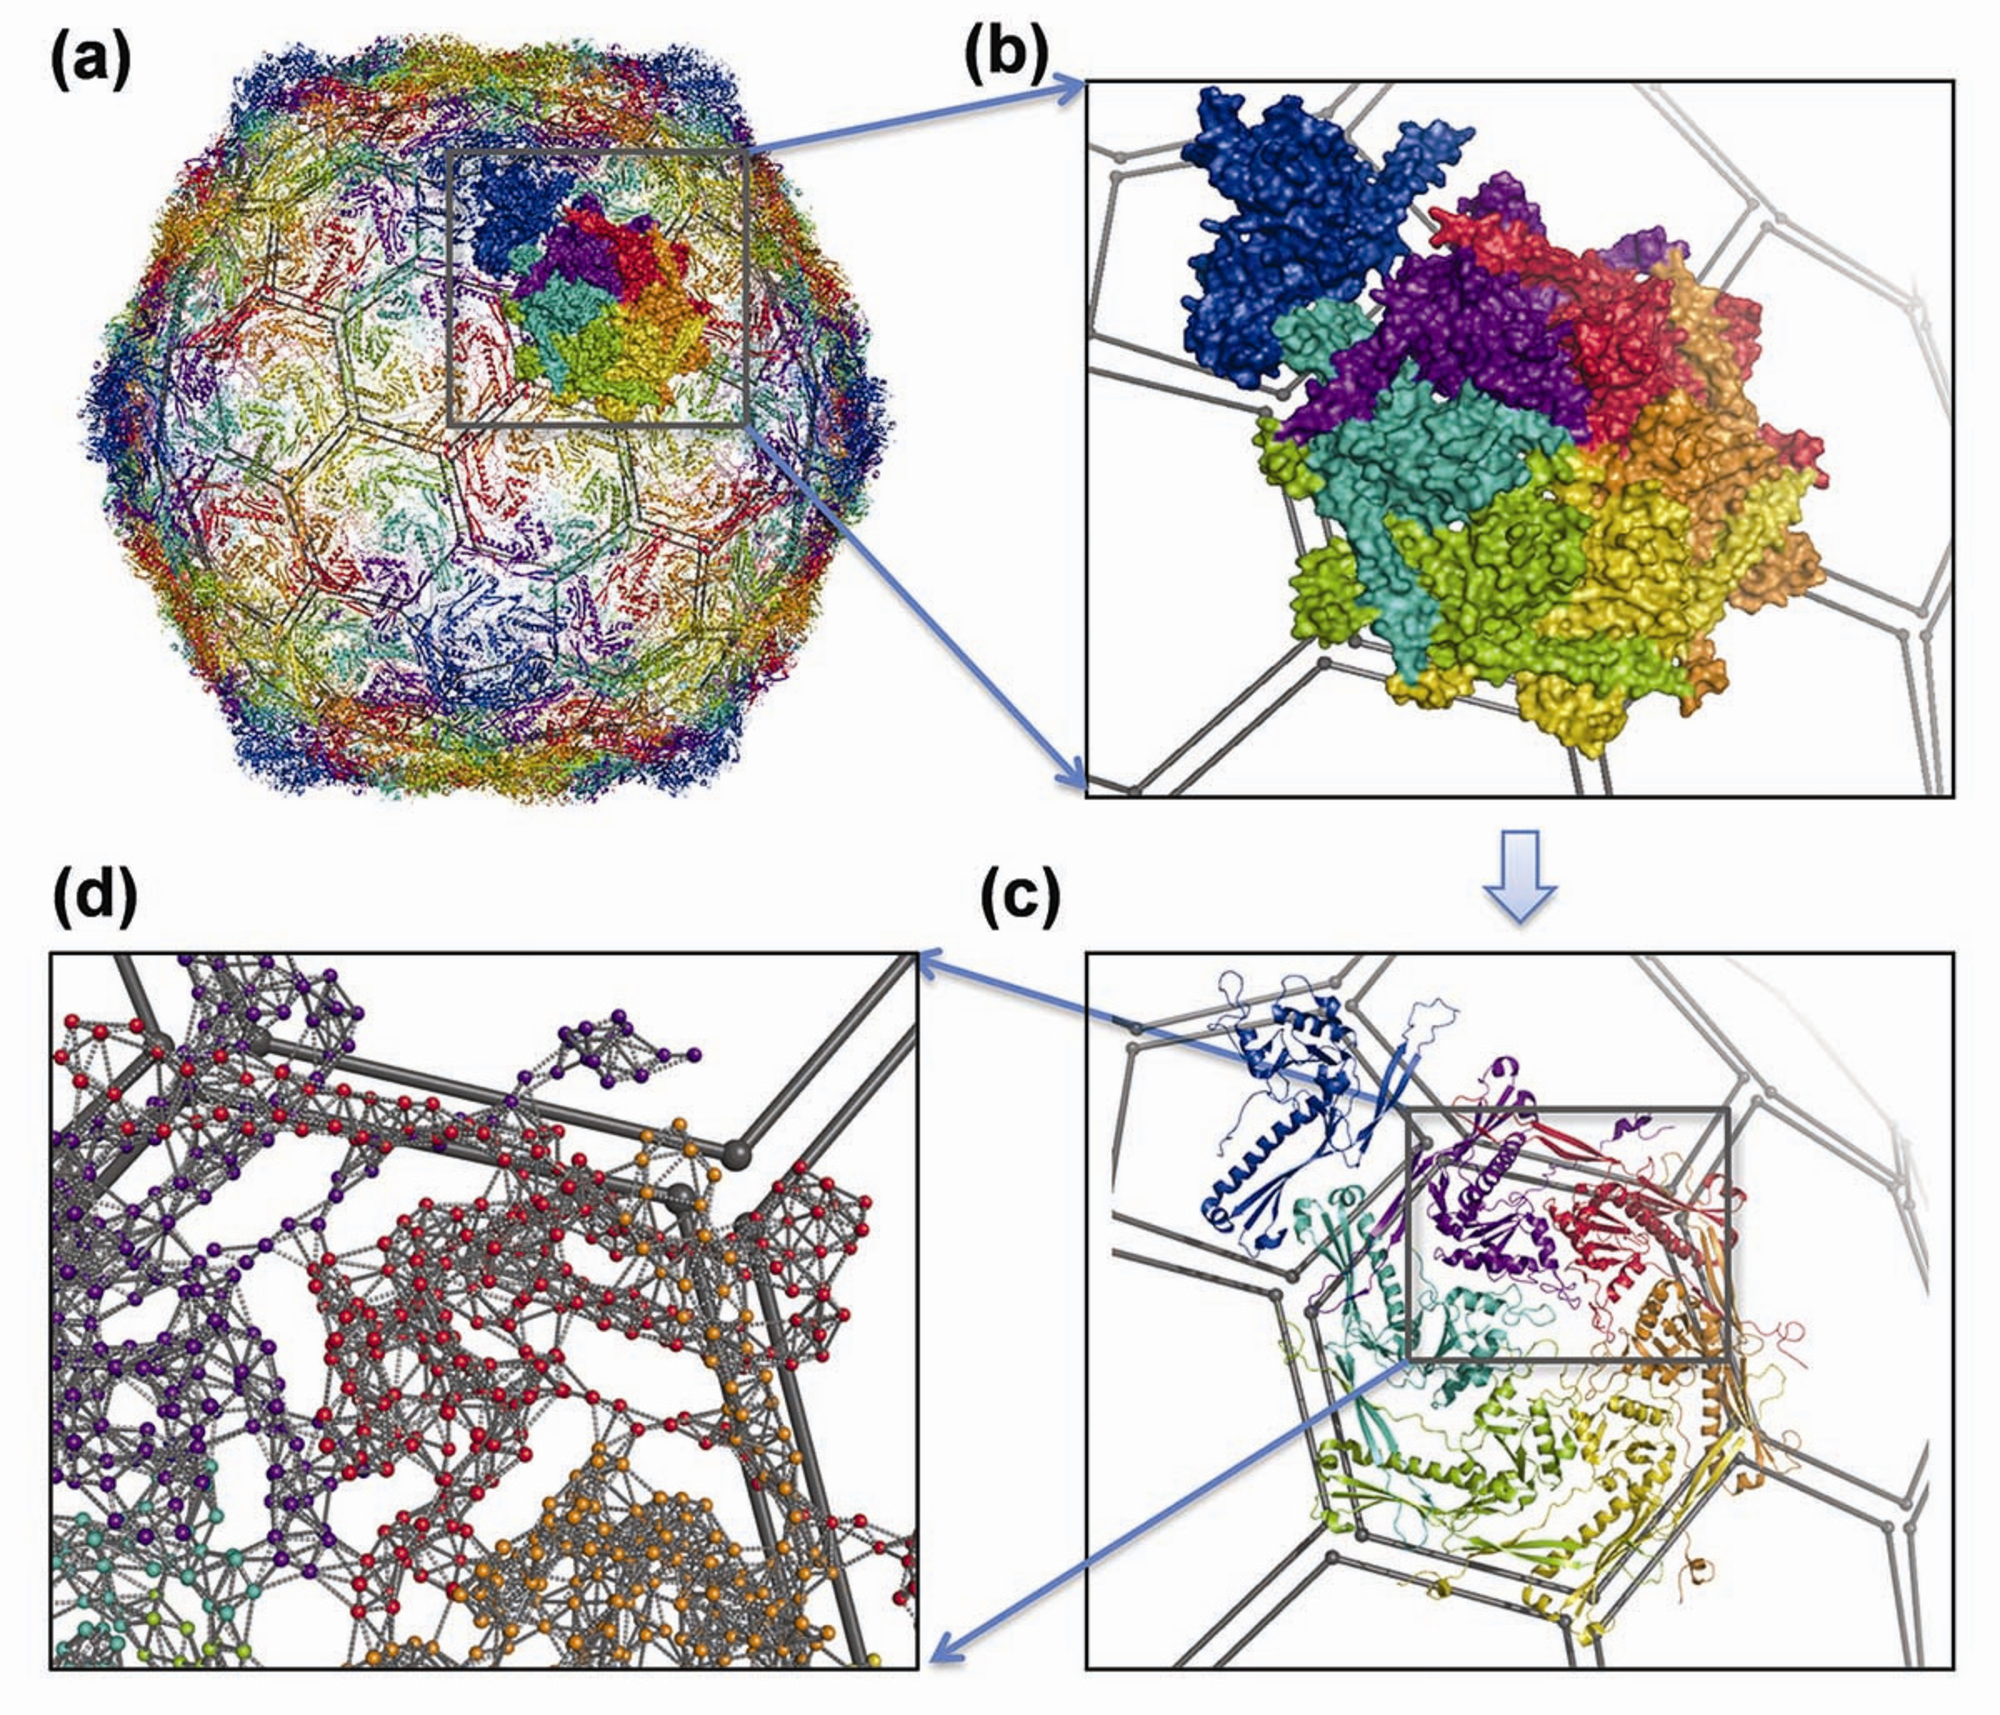
\includegraphics[scale=0.28]{Kap2/dibujo.pdf}%
\caption{ (a) Vista exterior de un c\'{a}pside v\'{i}rico HK97 coloreado por cada cadena, todas las prote\'{i}nas son id\'{e}nticas. (b) Vista del arreglo prote\'{i}nico en una cara del c\'{a}pside. (c) Vista de la estructura secundaria de las prote\'{i}nas (d) Esquema de cada prote\'{i}na mostrando cada uno de sus \'{a}tomos, las aristas de cada cara son carbonos $\alpha$ unidos por lados (ligaduras el\'{a}sticas). Tomado de \cite{Lezon2009}.} \label{fig:pan}
\end{figure}

La primera vez que se usaron los ENM en la investigaci\'{o}n de prote\'{i}nas fue gracias a Monique Tirion, ver \cite{Tirion1996}. Entre las prote\'{i}nas  investigadas se encuentran la actina G (C\'{o}digo PDB: 1atn) y la miosina H1 (C\'{o}digo PDB: 1my). La G-actina es modelada bien por los ENM.\\ 

Existen dos tipos de ENM: Modelos de redes anisotr\'{o}picas (ANM por sus siglas en ingl\'{e}s) y Modelos de Redes Gaussianas (GNM por sus siglas en ingl\'{e}s) los cuales se diferencian en el modelo de potencial usado.  El modelo de redes anisotr\'{o}picas inicialmente no usa el mismo potencial que el an\'{a}lisis de modos normales est\'{a}ndar sino que usa el potencial presente entre resortes tridimensionales, en la figura \cite{fig:ANM} se muestra que el potencial entre los resortes depende de la diferencia de distancias.\\
\begin{figure}
\centering
%LaTeX with PSTricks extensions
%%Creator: inkscape 0.48.5
%%Please note this file requires PSTricks extensions
\psset{xunit=.5pt,yunit=.5pt,runit=.5pt}
\begin{pspicture}(620.04998779,250.19999695)
{
\newrgbcolor{curcolor}{0 0 0}
\pscustom[linewidth=0.96809698,linecolor=curcolor]
{
\newpath
\moveto(240.48010465,176.5854835)
\curveto(240.48010465,166.38227921)(232.62614166,158.11094787)(222.93778733,158.11094787)
\curveto(213.24943299,158.11094787)(205.39547001,166.38227921)(205.39547001,176.5854835)
\curveto(205.39547001,186.78868779)(213.24943299,195.06001913)(222.93778733,195.06001913)
\curveto(232.62614166,195.06001913)(240.48010465,186.78868779)(240.48010465,176.5854835)
\closepath
}
}
{
\newrgbcolor{curcolor}{0 0 0}
\pscustom[linewidth=0.98306393,linecolor=curcolor]
{
\newpath
\moveto(346.60167259,174.05060899)
\curveto(346.60167259,163.85152441)(338.4997138,155.58353276)(328.50544114,155.58353276)
\curveto(318.51116849,155.58353276)(310.4092097,163.85152441)(310.4092097,174.05060899)
\curveto(310.4092097,184.24969356)(318.51116849,192.51768521)(328.50544114,192.51768521)
\curveto(338.4997138,192.51768521)(346.60167259,184.24969356)(346.60167259,174.05060899)
\closepath
}
}
{
\newrgbcolor{curcolor}{0 0 0}
\pscustom[linewidth=0.329673,linecolor=curcolor]
{
\newpath
\moveto(241.4713779,186.50210996)
\curveto(248.58644604,173.65845178)(240.8043424,167.42366304)(240.8043424,167.42366304)
\lineto(240.54394377,167.42366304)
}
}
{
\newrgbcolor{curcolor}{0 0 0}
\pscustom[linewidth=0.329673,linecolor=curcolor]
{
\newpath
\moveto(239.32625885,186.50211345)
\curveto(232.48912399,173.59610791)(240.5491609,167.42366653)(240.5491609,167.42366653)
\lineto(240.80464746,167.42918307)
}
}
{
\newrgbcolor{curcolor}{0 0 0}
\pscustom[linewidth=0.329673,linecolor=curcolor]
{
\newpath
\moveto(243.36542054,186.37741366)
\curveto(250.48048868,173.53375548)(242.69838504,167.29896674)(242.69838504,167.29896674)
\lineto(242.43798641,167.29896674)
}
}
{
\newrgbcolor{curcolor}{0 0 0}
\pscustom[linewidth=0.329673,linecolor=curcolor]
{
\newpath
\moveto(241.49543943,186.50589315)
\curveto(234.65830456,173.59988761)(242.44320353,167.29897023)(242.44320353,167.29897023)
\lineto(242.6986901,167.30448677)
}
}
{
\newrgbcolor{curcolor}{0 0 0}
\pscustom[linewidth=0.329673,linecolor=curcolor]
{
\newpath
\moveto(245.62626995,186.40660762)
\curveto(252.74133809,173.56294944)(244.95923446,167.3281607)(244.95923446,167.3281607)
\lineto(244.69883583,167.3281607)
}
}
{
\newrgbcolor{curcolor}{0 0 0}
\pscustom[linewidth=0.329673,linecolor=curcolor]
{
\newpath
\moveto(243.48115091,186.40661111)
\curveto(236.64401604,173.50060557)(244.70405295,167.32816419)(244.70405295,167.32816419)
\lineto(244.95953951,167.33368073)
}
}
{
\newrgbcolor{curcolor}{0 0 0}
\pscustom[linewidth=0.329673,linecolor=curcolor]
{
\newpath
\moveto(247.52031259,186.28191132)
\curveto(254.63538073,173.43825314)(246.85327709,167.20346439)(246.85327709,167.20346439)
\lineto(246.59287846,167.20346439)
}
}
{
\newrgbcolor{curcolor}{0 0 0}
\pscustom[linewidth=0.329673,linecolor=curcolor]
{
\newpath
\moveto(245.65033148,186.41039081)
\curveto(238.81319662,173.50438527)(246.59809559,167.20346788)(246.59809559,167.20346788)
\lineto(246.85358215,167.20898442)
}
}
{
\newrgbcolor{curcolor}{0 0 0}
\pscustom[linewidth=0.329673,linecolor=curcolor]
{
\newpath
\moveto(249.69439707,186.34047802)
\curveto(256.80946521,173.49681984)(249.02736158,167.2620311)(249.02736158,167.2620311)
\lineto(248.76696295,167.2620311)
}
}
{
\newrgbcolor{curcolor}{0 0 0}
\pscustom[linewidth=0.329673,linecolor=curcolor]
{
\newpath
\moveto(247.54927803,186.34048151)
\curveto(240.71214316,173.43447597)(248.77218007,167.26203459)(248.77218007,167.26203459)
\lineto(249.02766664,167.26755113)
}
}
{
\newrgbcolor{curcolor}{0 0 0}
\pscustom[linewidth=0.329673,linecolor=curcolor]
{
\newpath
\moveto(251.58843971,186.21578172)
\curveto(258.70350785,173.37212354)(250.92140421,167.1373348)(250.92140421,167.1373348)
\lineto(250.66100558,167.1373348)
}
}
{
\newrgbcolor{curcolor}{0 0 0}
\pscustom[linewidth=0.329673,linecolor=curcolor]
{
\newpath
\moveto(249.7184586,186.34426121)
\curveto(242.88132374,173.43825567)(250.66622271,167.13733829)(250.66622271,167.13733829)
\lineto(250.92170927,167.14285483)
}
}
{
\newrgbcolor{curcolor}{0 0 0}
\pscustom[linewidth=0.329673,linecolor=curcolor]
{
\newpath
\moveto(253.89672165,186.23026116)
\curveto(261.01178979,173.38660298)(253.22968615,167.15181423)(253.22968615,167.15181423)
\lineto(252.96928752,167.15181423)
}
}
{
\newrgbcolor{curcolor}{0 0 0}
\pscustom[linewidth=0.329673,linecolor=curcolor]
{
\newpath
\moveto(251.7516026,186.23026465)
\curveto(244.91446773,173.32425911)(252.97450464,167.15181773)(252.97450464,167.15181773)
\lineto(253.22999121,167.15733426)
}
}
{
\newrgbcolor{curcolor}{0 0 0}
\pscustom[linewidth=0.329673,linecolor=curcolor]
{
\newpath
\moveto(255.79076428,186.10556485)
\curveto(262.90583242,173.26190668)(255.12372878,167.02711793)(255.12372878,167.02711793)
\lineto(254.86333015,167.02711793)
}
}
{
\newrgbcolor{curcolor}{0 0 0}
\pscustom[linewidth=0.329673,linecolor=curcolor]
{
\newpath
\moveto(253.92078317,186.23404435)
\curveto(247.08364831,173.3280388)(254.86854728,167.02712142)(254.86854728,167.02712142)
\lineto(255.12403384,167.03263796)
}
}
{
\newrgbcolor{curcolor}{0 0 0}
\pscustom[linewidth=0.329673,linecolor=curcolor]
{
\newpath
\moveto(257.92891504,186.05391497)
\curveto(265.04398318,173.21025679)(257.26187955,166.97546805)(257.26187955,166.97546805)
\lineto(257.00148092,166.97546805)
}
}
{
\newrgbcolor{curcolor}{0 0 0}
\pscustom[linewidth=0.329673,linecolor=curcolor]
{
\newpath
\moveto(255.783796,186.05391846)
\curveto(248.94666113,173.14791292)(257.00669804,166.97547154)(257.00669804,166.97547154)
\lineto(257.26218461,166.98098808)
}
}
{
\newrgbcolor{curcolor}{0 0 0}
\pscustom[linewidth=0.329673,linecolor=curcolor]
{
\newpath
\moveto(259.82295768,185.92921867)
\curveto(266.93802582,173.08556049)(259.15592218,166.85077175)(259.15592218,166.85077175)
\lineto(258.89552355,166.85077175)
}
}
{
\newrgbcolor{curcolor}{0 0 0}
\pscustom[linewidth=0.329673,linecolor=curcolor]
{
\newpath
\moveto(257.95297657,186.05769816)
\curveto(251.11584171,173.15169262)(258.90074068,166.85077524)(258.90074068,166.85077524)
\lineto(259.15622724,166.85629178)
}
}
{
\newrgbcolor{curcolor}{0 0 0}
\pscustom[linewidth=0.329673,linecolor=curcolor]
{
\newpath
\moveto(262.03971955,185.92921923)
\curveto(269.15478769,173.08556105)(261.37268405,166.85077231)(261.37268405,166.85077231)
\lineto(261.11228542,166.85077231)
}
}
{
\newrgbcolor{curcolor}{0 0 0}
\pscustom[linewidth=0.329673,linecolor=curcolor]
{
\newpath
\moveto(259.8946005,185.92922272)
\curveto(253.05746564,173.02321718)(261.11750255,166.8507758)(261.11750255,166.8507758)
\lineto(261.37298911,166.85629234)
}
}
{
\newrgbcolor{curcolor}{0 0 0}
\pscustom[linewidth=0.329673,linecolor=curcolor]
{
\newpath
\moveto(263.93376218,185.80452293)
\curveto(271.04883032,172.96086475)(263.26672669,166.72607601)(263.26672669,166.72607601)
\lineto(263.00632806,166.72607601)
}
}
{
\newrgbcolor{curcolor}{0 0 0}
\pscustom[linewidth=0.329673,linecolor=curcolor]
{
\newpath
\moveto(262.06378108,185.93300242)
\curveto(255.22664621,173.02699688)(263.01154518,166.7260795)(263.01154518,166.7260795)
\lineto(263.26703175,166.73159604)
}
}
{
\newrgbcolor{curcolor}{0 0 0}
\pscustom[linewidth=0.329673,linecolor=curcolor]
{
\newpath
\moveto(266.19987413,185.97693771)
\curveto(273.31494227,173.13327953)(265.53283863,166.89849079)(265.53283863,166.89849079)
\lineto(265.27244,166.89849079)
}
}
{
\newrgbcolor{curcolor}{0 0 0}
\pscustom[linewidth=0.329673,linecolor=curcolor]
{
\newpath
\moveto(264.05475508,185.9769412)
\curveto(257.21762022,173.07093566)(265.27765713,166.89849428)(265.27765713,166.89849428)
\lineto(265.53314369,166.90401082)
}
}
{
\newrgbcolor{curcolor}{0 0 0}
\pscustom[linewidth=0.329673,linecolor=curcolor]
{
\newpath
\moveto(268.09391676,185.85224141)
\curveto(275.2089849,173.00858323)(267.42688127,166.77379449)(267.42688127,166.77379449)
\lineto(267.16648264,166.77379449)
}
}
{
\newrgbcolor{curcolor}{0 0 0}
\pscustom[linewidth=0.329673,linecolor=curcolor]
{
\newpath
\moveto(266.22393566,185.9807209)
\curveto(259.38680079,173.07471536)(267.17169976,166.77379798)(267.17169976,166.77379798)
\lineto(267.42718633,166.77931452)
}
}
{
\newrgbcolor{curcolor}{0 0 0}
\pscustom[linewidth=0.329673,linecolor=curcolor]
{
\newpath
\moveto(270.24783968,185.87756833)
\curveto(277.36290782,173.03391015)(269.58080418,166.79912141)(269.58080418,166.79912141)
\lineto(269.32040555,166.79912141)
}
}
{
\newrgbcolor{curcolor}{0 0 0}
\pscustom[linewidth=0.329673,linecolor=curcolor]
{
\newpath
\moveto(268.10272063,185.87757182)
\curveto(261.26558576,172.97156628)(269.32562268,166.7991249)(269.32562268,166.7991249)
\lineto(269.58110924,166.80464144)
}
}
{
\newrgbcolor{curcolor}{0 0 0}
\pscustom[linewidth=0.329673,linecolor=curcolor]
{
\newpath
\moveto(272.14188231,185.75287203)
\curveto(279.25695045,172.90921385)(271.47484682,166.67442511)(271.47484682,166.67442511)
\lineto(271.21444819,166.67442511)
}
}
{
\newrgbcolor{curcolor}{0 0 0}
\pscustom[linewidth=0.329673,linecolor=curcolor]
{
\newpath
\moveto(270.27190121,185.88135152)
\curveto(263.43476634,172.97534598)(271.21966531,166.6744286)(271.21966531,166.6744286)
\lineto(271.47515188,166.67994514)
}
}
{
\newrgbcolor{curcolor}{0 0 0}
\pscustom[linewidth=0.329673,linecolor=curcolor]
{
\newpath
\moveto(274.36817913,185.88826567)
\curveto(281.48324727,173.04460749)(273.70114364,166.80981875)(273.70114364,166.80981875)
\lineto(273.440745,166.80981875)
}
}
{
\newrgbcolor{curcolor}{0 0 0}
\pscustom[linewidth=0.329673,linecolor=curcolor]
{
\newpath
\moveto(272.22306008,185.88826916)
\curveto(265.38592522,172.98226362)(273.44596213,166.80982224)(273.44596213,166.80982224)
\lineto(273.70144869,166.81533878)
}
}
{
\newrgbcolor{curcolor}{0 0 0}
\pscustom[linewidth=0.329673,linecolor=curcolor]
{
\newpath
\moveto(276.26222177,185.76356937)
\curveto(283.37728991,172.91991119)(275.59518627,166.68512244)(275.59518627,166.68512244)
\lineto(275.33478764,166.68512244)
}
}
{
\newrgbcolor{curcolor}{0 0 0}
\pscustom[linewidth=0.329673,linecolor=curcolor]
{
\newpath
\moveto(274.39224066,185.89204886)
\curveto(267.55510579,172.98604332)(275.34000476,166.68512593)(275.34000476,166.68512593)
\lineto(275.59549133,166.69064247)
}
}
{
\newrgbcolor{curcolor}{0 0 0}
\pscustom[linewidth=0.329673,linecolor=curcolor]
{
\newpath
\moveto(278.46665678,185.65370495)
\curveto(285.58172492,172.81004677)(277.79962128,166.57525803)(277.79962128,166.57525803)
\lineto(277.53922265,166.57525803)
}
}
{
\newrgbcolor{curcolor}{0 0 0}
\pscustom[linewidth=0.329673,linecolor=curcolor]
{
\newpath
\moveto(276.32153773,185.65370844)
\curveto(269.48440287,172.7477029)(277.54443978,166.57526152)(277.54443978,166.57526152)
\lineto(277.79992634,166.58077806)
}
}
{
\newrgbcolor{curcolor}{0 0 0}
\pscustom[linewidth=0.329673,linecolor=curcolor]
{
\newpath
\moveto(280.36069942,185.52900865)
\curveto(287.47576756,172.68535047)(279.69366392,166.45056172)(279.69366392,166.45056172)
\lineto(279.43326529,166.45056172)
}
}
{
\newrgbcolor{curcolor}{0 0 0}
\pscustom[linewidth=0.329673,linecolor=curcolor]
{
\newpath
\moveto(278.49071831,185.65748814)
\curveto(271.65358344,172.7514826)(279.43848241,166.45056522)(279.43848241,166.45056522)
\lineto(279.69396898,166.45608175)
}
}
{
\newrgbcolor{curcolor}{0 0 0}
\pscustom[linewidth=0.329673,linecolor=curcolor]
{
\newpath
\moveto(282.62155159,185.55820249)
\curveto(289.73661973,172.71454431)(281.95451609,166.47975557)(281.95451609,166.47975557)
\lineto(281.69411746,166.47975557)
}
}
{
\newrgbcolor{curcolor}{0 0 0}
\pscustom[linewidth=0.329673,linecolor=curcolor]
{
\newpath
\moveto(280.47643254,185.55820598)
\curveto(273.63929768,172.65220044)(281.69933459,166.47975906)(281.69933459,166.47975906)
\lineto(281.95482115,166.4852756)
}
}
{
\newrgbcolor{curcolor}{0 0 0}
\pscustom[linewidth=0.329673,linecolor=curcolor]
{
\newpath
\moveto(284.51559423,185.43350619)
\curveto(291.63066237,172.58984801)(283.84855873,166.35505926)(283.84855873,166.35505926)
\lineto(283.5881601,166.35505926)
}
}
{
\newrgbcolor{curcolor}{0 0 0}
\pscustom[linewidth=0.329673,linecolor=curcolor]
{
\newpath
\moveto(282.64561312,185.56198568)
\curveto(275.80847825,172.65598014)(283.59337722,166.35506276)(283.59337722,166.35506276)
\lineto(283.84886379,166.36057929)
}
}
{
\newrgbcolor{curcolor}{0 0 0}
\pscustom[linewidth=0.329673,linecolor=curcolor]
{
\newpath
\moveto(286.68967591,185.49207385)
\curveto(293.80474405,172.64841567)(286.02264041,166.41362693)(286.02264041,166.41362693)
\lineto(285.76224178,166.41362693)
}
}
{
\newrgbcolor{curcolor}{0 0 0}
\pscustom[linewidth=0.329673,linecolor=curcolor]
{
\newpath
\moveto(284.54455686,185.49207734)
\curveto(277.707422,172.5860718)(285.76745891,166.41363042)(285.76745891,166.41363042)
\lineto(286.02294547,166.41914696)
}
}
{
\newrgbcolor{curcolor}{0 0 0}
\pscustom[linewidth=0.329673,linecolor=curcolor]
{
\newpath
\moveto(288.58371855,185.36737755)
\curveto(295.69878668,172.52371937)(287.91668305,166.28893063)(287.91668305,166.28893063)
\lineto(287.65628442,166.28893063)
}
}
{
\newrgbcolor{curcolor}{0 0 0}
\pscustom[linewidth=0.329673,linecolor=curcolor]
{
\newpath
\moveto(286.71373744,185.49585704)
\curveto(279.87660257,172.5898515)(287.66150154,166.28893412)(287.66150154,166.28893412)
\lineto(287.91698811,166.29445066)
}
}
{
\newrgbcolor{curcolor}{0 0 0}
\pscustom[linewidth=0.329673,linecolor=curcolor]
{
\newpath
\moveto(290.8920011,185.38185829)
\curveto(298.00706924,172.53820011)(290.22496561,166.30341137)(290.22496561,166.30341137)
\lineto(289.96456698,166.30341137)
}
}
{
\newrgbcolor{curcolor}{0 0 0}
\pscustom[linewidth=0.329673,linecolor=curcolor]
{
\newpath
\moveto(288.74688206,185.38186178)
\curveto(281.90974719,172.47585624)(289.9697841,166.30341486)(289.9697841,166.30341486)
\lineto(290.22527066,166.3089314)
}
}
{
\newrgbcolor{curcolor}{0 0 0}
\pscustom[linewidth=0.329673,linecolor=curcolor]
{
\newpath
\moveto(292.78604374,185.25716199)
\curveto(299.90111188,172.41350381)(292.11900824,166.17871507)(292.11900824,166.17871507)
\lineto(291.85860961,166.17871507)
}
}
{
\newrgbcolor{curcolor}{0 0 0}
\pscustom[linewidth=0.329673,linecolor=curcolor]
{
\newpath
\moveto(290.91606263,185.38564148)
\curveto(284.07892776,172.47963594)(291.86382673,166.17871856)(291.86382673,166.17871856)
\lineto(292.1193133,166.1842351)
}
}
{
\newrgbcolor{curcolor}{0 0 0}
\pscustom[linewidth=0.329673,linecolor=curcolor]
{
\newpath
\moveto(294.92419388,185.20551061)
\curveto(302.03926202,172.36185243)(294.25715838,166.12706368)(294.25715838,166.12706368)
\lineto(293.99675975,166.12706368)
}
}
{
\newrgbcolor{curcolor}{0 0 0}
\pscustom[linewidth=0.329673,linecolor=curcolor]
{
\newpath
\moveto(292.77907483,185.2055141)
\curveto(285.94193997,172.29950855)(294.00197688,166.12706717)(294.00197688,166.12706717)
\lineto(294.25746344,166.13258371)
}
}
{
\newrgbcolor{curcolor}{0 0 0}
\pscustom[linewidth=0.329673,linecolor=curcolor]
{
\newpath
\moveto(296.81823651,185.0808143)
\curveto(303.93330465,172.23715613)(296.15120102,166.00236738)(296.15120102,166.00236738)
\lineto(295.89080239,166.00236738)
}
}
{
\newrgbcolor{curcolor}{0 0 0}
\pscustom[linewidth=0.329673,linecolor=curcolor]
{
\newpath
\moveto(294.94825541,185.2092938)
\curveto(288.11112054,172.30328825)(295.89601951,166.00237087)(295.89601951,166.00237087)
\lineto(296.15150608,166.00788741)
}
}
{
\newrgbcolor{curcolor}{0 0 0}
\pscustom[linewidth=0.329673,linecolor=curcolor]
{
\newpath
\moveto(299.03499839,185.08081588)
\curveto(306.15006652,172.2371577)(298.36796289,166.00236896)(298.36796289,166.00236896)
\lineto(298.10756426,166.00236896)
}
}
{
\newrgbcolor{curcolor}{0 0 0}
\pscustom[linewidth=0.329673,linecolor=curcolor]
{
\newpath
\moveto(296.88987934,185.08081937)
\curveto(290.05274447,172.17481383)(298.11278138,166.00237245)(298.11278138,166.00237245)
\lineto(298.36826795,166.00788899)
}
}
{
\newrgbcolor{curcolor}{0 0 0}
\pscustom[linewidth=0.329673,linecolor=curcolor]
{
\newpath
\moveto(300.92904102,184.95611958)
\curveto(308.04410916,172.1124614)(300.26200552,165.87767265)(300.26200552,165.87767265)
\lineto(300.00160689,165.87767265)
}
}
{
\newrgbcolor{curcolor}{0 0 0}
\pscustom[linewidth=0.329673,linecolor=curcolor]
{
\newpath
\moveto(299.05905991,185.08459907)
\curveto(292.22192505,172.17859353)(300.00682402,165.87767615)(300.00682402,165.87767615)
\lineto(300.26231058,165.88319268)
}
}
{
\newrgbcolor{curcolor}{0 0 0}
\pscustom[linewidth=0.329673,linecolor=curcolor]
{
\newpath
\moveto(303.1951539,185.12853394)
\curveto(310.31022204,172.28487576)(302.5281184,166.05008702)(302.5281184,166.05008702)
\lineto(302.26771977,166.05008702)
}
}
{
\newrgbcolor{curcolor}{0 0 0}
\pscustom[linewidth=0.329673,linecolor=curcolor]
{
\newpath
\moveto(301.05003485,185.12853743)
\curveto(294.21289998,172.22253189)(302.27293689,166.05009051)(302.27293689,166.05009051)
\lineto(302.52842346,166.05560705)
}
}
{
\newrgbcolor{curcolor}{0 0 0}
\pscustom[linewidth=0.329673,linecolor=curcolor]
{
\newpath
\moveto(305.08919653,185.00383764)
\curveto(312.20426467,172.16017946)(304.42216104,165.92539071)(304.42216104,165.92539071)
\lineto(304.16176241,165.92539071)
}
}
{
\newrgbcolor{curcolor}{0 0 0}
\pscustom[linewidth=0.329673,linecolor=curcolor]
{
\newpath
\moveto(303.21921543,185.13231713)
\curveto(296.38208056,172.22631159)(304.16697953,165.92539421)(304.16697953,165.92539421)
\lineto(304.42246609,165.93091075)
}
}
{
\newrgbcolor{curcolor}{0 0 0}
\pscustom[linewidth=0.329673,linecolor=curcolor]
{
\newpath
\moveto(307.24311945,185.02916641)
\curveto(314.35818759,172.18550823)(306.57608395,165.95071949)(306.57608395,165.95071949)
\lineto(306.31568532,165.95071949)
}
}
{
\newrgbcolor{curcolor}{0 0 0}
\pscustom[linewidth=0.329673,linecolor=curcolor]
{
\newpath
\moveto(305.0980004,185.0291699)
\curveto(298.26086553,172.12316436)(306.32090244,165.95072298)(306.32090244,165.95072298)
\lineto(306.57638901,165.95623952)
}
}
{
\newrgbcolor{curcolor}{0 0 0}
\pscustom[linewidth=0.329673,linecolor=curcolor]
{
\newpath
\moveto(309.13716208,184.90447011)
\curveto(316.25223022,172.06081193)(308.47012659,165.82602319)(308.47012659,165.82602319)
\lineto(308.20972796,165.82602319)
}
}
{
\newrgbcolor{curcolor}{0 0 0}
\pscustom[linewidth=0.329673,linecolor=curcolor]
{
\newpath
\moveto(307.26718098,185.0329496)
\curveto(300.43004611,172.12694406)(308.21494508,165.82602668)(308.21494508,165.82602668)
\lineto(308.47043164,165.83154322)
}
}
{
\newrgbcolor{curcolor}{0 0 0}
\pscustom[linewidth=0.329673,linecolor=curcolor]
{
\newpath
\moveto(311.36345859,185.03986081)
\curveto(318.47852673,172.19620264)(310.69642309,165.96141389)(310.69642309,165.96141389)
\lineto(310.43602446,165.96141389)
}
}
{
\newrgbcolor{curcolor}{0 0 0}
\pscustom[linewidth=0.329673,linecolor=curcolor]
{
\newpath
\moveto(309.21833954,185.03986431)
\curveto(302.38120468,172.13385876)(310.44124159,165.96141738)(310.44124159,165.96141738)
\lineto(310.69672815,165.96693392)
}
}
{
\newrgbcolor{curcolor}{0 0 0}
\pscustom[linewidth=0.329673,linecolor=curcolor]
{
\newpath
\moveto(313.25750123,184.91516451)
\curveto(320.37256937,172.07150633)(312.59046573,165.83671759)(312.59046573,165.83671759)
\lineto(312.3300671,165.83671759)
}
}
{
\newrgbcolor{curcolor}{0 0 0}
\pscustom[linewidth=0.329673,linecolor=curcolor]
{
\newpath
\moveto(311.38752012,185.043644)
\curveto(304.55038525,172.13763846)(312.33528422,165.83672108)(312.33528422,165.83672108)
\lineto(312.59077079,165.84223762)
}
}
{
\newrgbcolor{curcolor}{0 0 0}
\pscustom[linewidth=0.99451757,linecolor=curcolor]
{
\newpath
\moveto(249.49099243,128.11175157)
\curveto(246.84433855,118.57485364)(236.27413795,112.43969329)(225.88178859,114.40848739)
\curveto(215.48943924,116.3772815)(209.2103124,125.70448778)(211.85696628,135.24138572)
\curveto(214.50362016,144.77828365)(225.07382076,150.913444)(235.46617012,148.9446499)
\curveto(245.85851947,146.97585579)(252.1376463,137.64864951)(249.49099243,128.11175157)
\closepath
}
}
{
\newrgbcolor{curcolor}{0 0 0}
\pscustom[linewidth=0.95157243,linecolor=curcolor]
{
\newpath
\moveto(367.33185651,105.90041566)
\curveto(364.91177965,96.3519429)(355.24648188,90.20933606)(345.74380973,92.18051929)
\curveto(336.24113758,94.15170252)(330.49955967,103.49022883)(332.91963653,113.0387016)
\curveto(335.3397134,122.58717436)(345.00501117,128.7297812)(354.50768332,126.75859797)
\curveto(364.01035547,124.78741474)(369.75193338,115.44888843)(367.33185651,105.90041566)
\closepath
}
}
{
\newrgbcolor{curcolor}{0 0 0}
\pscustom[linewidth=0.35938292,linecolor=curcolor]
{
\newpath
\moveto(251.41734966,138.64167701)
\curveto(256.44401602,124.82965504)(245.55472408,120.63382247)(245.55472408,120.63382247)
\lineto(245.24581018,120.69197024)
}
}
{
\newrgbcolor{curcolor}{0 0 0}
\pscustom[linewidth=0.35938292,linecolor=curcolor]
{
\newpath
\moveto(248.87257112,139.12069157)
\curveto(237.33100533,128.36490105)(245.25200025,120.69080856)(245.25200025,120.69080856)
\lineto(245.55655328,120.63900772)
}
}
{
\newrgbcolor{curcolor}{0 0 0}
\pscustom[linewidth=0.35938292,linecolor=curcolor]
{
\newpath
\moveto(253.63112829,138.10005938)
\curveto(258.65779465,124.28803742)(247.76850271,120.09220485)(247.76850271,120.09220485)
\lineto(247.45958881,120.15035261)
}
}
{
\newrgbcolor{curcolor}{0 0 0}
\pscustom[linewidth=0.35938292,linecolor=curcolor]
{
\newpath
\moveto(251.44689975,138.63990443)
\curveto(239.90533396,127.88411391)(247.46577888,120.14919093)(247.46577888,120.14919093)
\lineto(247.77033191,120.0973901)
}
}
{
\newrgbcolor{curcolor}{0 0 0}
\pscustom[linewidth=0.35938292,linecolor=curcolor]
{
\newpath
\moveto(256.32096019,137.62298888)
\curveto(261.34762654,123.81096692)(250.45833461,119.61513435)(250.45833461,119.61513435)
\lineto(250.14942071,119.67328211)
}
}
{
\newrgbcolor{curcolor}{0 0 0}
\pscustom[linewidth=0.35938292,linecolor=curcolor]
{
\newpath
\moveto(253.77618165,138.10200344)
\curveto(242.23461586,127.34621292)(250.15561077,119.67212043)(250.15561077,119.67212043)
\lineto(250.4601638,119.6203196)
}
}
{
\newrgbcolor{curcolor}{0 0 0}
\pscustom[linewidth=0.35938292,linecolor=curcolor]
{
\newpath
\moveto(258.53473882,137.08137126)
\curveto(263.56140518,123.26934929)(252.67211324,119.07351672)(252.67211324,119.07351672)
\lineto(252.36319934,119.13166448)
}
}
{
\newrgbcolor{curcolor}{0 0 0}
\pscustom[linewidth=0.35938292,linecolor=curcolor]
{
\newpath
\moveto(256.35051028,137.62121631)
\curveto(244.80894449,126.86542579)(252.36938941,119.13050281)(252.36938941,119.13050281)
\lineto(252.67394244,119.07870197)
}
}
{
\newrgbcolor{curcolor}{0 0 0}
\pscustom[linewidth=0.35938292,linecolor=curcolor]
{
\newpath
\moveto(261.12944816,136.65162942)
\curveto(266.15611451,122.83960746)(255.26682258,118.64377489)(255.26682258,118.64377489)
\lineto(254.95790868,118.70192265)
}
}
{
\newrgbcolor{curcolor}{0 0 0}
\pscustom[linewidth=0.35938292,linecolor=curcolor]
{
\newpath
\moveto(258.58466962,137.13064398)
\curveto(247.04310383,126.37485346)(254.96409874,118.70076097)(254.96409874,118.70076097)
\lineto(255.26865177,118.64896014)
}
}
{
\newrgbcolor{curcolor}{0 0 0}
\pscustom[linewidth=0.35938292,linecolor=curcolor]
{
\newpath
\moveto(263.34322679,136.1100118)
\curveto(268.36989315,122.29798983)(257.48060121,118.10215726)(257.48060121,118.10215726)
\lineto(257.17168731,118.16030502)
}
}
{
\newrgbcolor{curcolor}{0 0 0}
\pscustom[linewidth=0.35938292,linecolor=curcolor]
{
\newpath
\moveto(261.15899825,136.64985685)
\curveto(249.61743246,125.89406633)(257.17787738,118.15914335)(257.17787738,118.15914335)
\lineto(257.48243041,118.10734251)
}
}
{
\newrgbcolor{curcolor}{0 0 0}
\pscustom[linewidth=0.35938292,linecolor=curcolor]
{
\newpath
\moveto(266.08541711,135.60834579)
\curveto(271.11208346,121.79632382)(260.22279153,117.60049125)(260.22279153,117.60049125)
\lineto(259.91387763,117.65863901)
}
}
{
\newrgbcolor{curcolor}{0 0 0}
\pscustom[linewidth=0.35938292,linecolor=curcolor]
{
\newpath
\moveto(263.54063857,136.08736035)
\curveto(251.99907278,125.33156983)(259.92006769,117.65747734)(259.92006769,117.65747734)
\lineto(260.22462073,117.6056765)
}
}
{
\newrgbcolor{curcolor}{0 0 0}
\pscustom[linewidth=0.35938292,linecolor=curcolor]
{
\newpath
\moveto(268.29919574,135.06672816)
\curveto(273.3258621,121.2547062)(262.43657016,117.05887363)(262.43657016,117.05887363)
\lineto(262.12765626,117.11702139)
}
}
{
\newrgbcolor{curcolor}{0 0 0}
\pscustom[linewidth=0.35938292,linecolor=curcolor]
{
\newpath
\moveto(266.1149672,135.60657321)
\curveto(254.57340141,124.85078269)(262.13384633,117.11585971)(262.13384633,117.11585971)
\lineto(262.43839936,117.06405888)
}
}
{
\newrgbcolor{curcolor}{0 0 0}
\pscustom[linewidth=0.35938292,linecolor=curcolor]
{
\newpath
\moveto(270.82197941,134.54011819)
\curveto(275.84864576,120.72809622)(264.95935383,116.53226365)(264.95935383,116.53226365)
\lineto(264.65043993,116.59041141)
}
}
{
\newrgbcolor{curcolor}{0 0 0}
\pscustom[linewidth=0.35938292,linecolor=curcolor]
{
\newpath
\moveto(268.27720086,135.01913274)
\curveto(256.73563508,124.26334222)(264.65662999,116.58924974)(264.65662999,116.58924974)
\lineto(264.96118302,116.5374489)
}
}
{
\newrgbcolor{curcolor}{0 0 0}
\pscustom[linewidth=0.35938292,linecolor=curcolor]
{
\newpath
\moveto(273.03575804,133.99850056)
\curveto(278.06242439,120.18647859)(267.17313246,115.99064603)(267.17313246,115.99064603)
\lineto(266.86421856,116.04879379)
}
}
{
\newrgbcolor{curcolor}{0 0 0}
\pscustom[linewidth=0.35938292,linecolor=curcolor]
{
\newpath
\moveto(270.8515295,134.53834561)
\curveto(259.30996371,123.78255509)(266.87040862,116.04763211)(266.87040862,116.04763211)
\lineto(267.17496165,115.99583127)
}
}
{
\newrgbcolor{curcolor}{0 0 0}
\pscustom[linewidth=0.35938292,linecolor=curcolor]
{
\newpath
\moveto(275.66552836,133.50349181)
\curveto(280.69219472,119.69146985)(269.80290278,115.49563728)(269.80290278,115.49563728)
\lineto(269.49398888,115.55378504)
}
}
{
\newrgbcolor{curcolor}{0 0 0}
\pscustom[linewidth=0.35938292,linecolor=curcolor]
{
\newpath
\moveto(273.12074982,133.98250637)
\curveto(261.57918403,123.22671585)(269.50017895,115.55262336)(269.50017895,115.55262336)
\lineto(269.80473198,115.50082253)
}
}
{
\newrgbcolor{curcolor}{0 0 0}
\pscustom[linewidth=0.35938292,linecolor=curcolor]
{
\newpath
\moveto(277.879307,132.96187419)
\curveto(282.90597335,119.14985222)(272.01668142,114.95401965)(272.01668142,114.95401965)
\lineto(271.70776752,115.01216742)
}
}
{
\newrgbcolor{curcolor}{0 0 0}
\pscustom[linewidth=0.35938292,linecolor=curcolor]
{
\newpath
\moveto(275.69507846,133.50171924)
\curveto(264.15351267,122.74592872)(271.71395758,115.01100574)(271.71395758,115.01100574)
\lineto(272.01851061,114.9592049)
}
}
{
\newrgbcolor{curcolor}{0 0 0}
\pscustom[linewidth=0.35938292,linecolor=curcolor]
{
\newpath
\moveto(280.61345196,132.61993067)
\curveto(285.64011831,118.8079087)(274.75082638,114.61207613)(274.75082638,114.61207613)
\lineto(274.44191248,114.67022389)
}
}
{
\newrgbcolor{curcolor}{0 0 0}
\pscustom[linewidth=0.35938292,linecolor=curcolor]
{
\newpath
\moveto(278.06867341,133.09894522)
\curveto(266.52710762,122.3431547)(274.44810254,114.66906222)(274.44810254,114.66906222)
\lineto(274.75265557,114.61726138)
}
}
{
\newrgbcolor{curcolor}{0 0 0}
\pscustom[linewidth=0.35938292,linecolor=curcolor]
{
\newpath
\moveto(282.82723059,132.07831304)
\curveto(287.85389694,118.26629107)(276.96460501,114.07045851)(276.96460501,114.07045851)
\lineto(276.65569111,114.12860627)
}
}
{
\newrgbcolor{curcolor}{0 0 0}
\pscustom[linewidth=0.35938292,linecolor=curcolor]
{
\newpath
\moveto(280.64300205,132.61815809)
\curveto(269.10143626,121.86236757)(276.66188117,114.12744459)(276.66188117,114.12744459)
\lineto(276.9664342,114.07564375)
}
}
{
\newrgbcolor{curcolor}{0 0 0}
\pscustom[linewidth=0.35938292,linecolor=curcolor]
{
\newpath
\moveto(285.38918643,131.62143931)
\curveto(290.41585278,117.80941734)(279.52656085,113.61358477)(279.52656085,113.61358477)
\lineto(279.21764695,113.67173253)
}
}
{
\newrgbcolor{curcolor}{0 0 0}
\pscustom[linewidth=0.35938292,linecolor=curcolor]
{
\newpath
\moveto(282.84440789,132.10045386)
\curveto(271.3028421,121.34466334)(279.22383701,113.67057086)(279.22383701,113.67057086)
\lineto(279.52839004,113.61877002)
}
}
{
\newrgbcolor{curcolor}{0 0 0}
\pscustom[linewidth=0.35938292,linecolor=curcolor]
{
\newpath
\moveto(287.60296506,131.07982168)
\curveto(292.62963142,117.26779972)(281.74033948,113.07196715)(281.74033948,113.07196715)
\lineto(281.43142558,113.13011491)
}
}
{
\newrgbcolor{curcolor}{0 0 0}
\pscustom[linewidth=0.35938292,linecolor=curcolor]
{
\newpath
\moveto(285.41873652,131.61966673)
\curveto(273.87717073,120.86387621)(281.43761565,113.12895323)(281.43761565,113.12895323)
\lineto(281.74216868,113.0771524)
}
}
{
\newrgbcolor{curcolor}{0 0 0}
\pscustom[linewidth=0.35938292,linecolor=curcolor]
{
\newpath
\moveto(290.28003615,130.71153626)
\curveto(295.3067025,116.8995143)(284.41741057,112.70368173)(284.41741057,112.70368173)
\lineto(284.10849667,112.76182949)
}
}
{
\newrgbcolor{curcolor}{0 0 0}
\pscustom[linewidth=0.35938292,linecolor=curcolor]
{
\newpath
\moveto(287.73525761,131.19055082)
\curveto(276.19369182,120.4347603)(284.11468673,112.76066781)(284.11468673,112.76066781)
\lineto(284.41923976,112.70886698)
}
}
{
\newrgbcolor{curcolor}{0 0 0}
\pscustom[linewidth=0.35938292,linecolor=curcolor]
{
\newpath
\moveto(292.49381478,130.16991864)
\curveto(297.52048114,116.35789667)(286.6311892,112.1620641)(286.6311892,112.1620641)
\lineto(286.3222753,112.22021186)
}
}
{
\newrgbcolor{curcolor}{0 0 0}
\pscustom[linewidth=0.35938292,linecolor=curcolor]
{
\newpath
\moveto(290.30958624,130.70976369)
\curveto(278.76802045,119.95397317)(286.32846537,112.21905019)(286.32846537,112.21905019)
\lineto(286.6330184,112.16724935)
}
}
{
\newrgbcolor{curcolor}{0 0 0}
\pscustom[linewidth=0.35938292,linecolor=curcolor]
{
\newpath
\moveto(295.07975799,129.57310489)
\curveto(300.10642435,115.76108293)(289.21713241,111.56525036)(289.21713241,111.56525036)
\lineto(288.90821851,111.62339812)
}
}
{
\newrgbcolor{curcolor}{0 0 0}
\pscustom[linewidth=0.35938292,linecolor=curcolor]
{
\newpath
\moveto(292.53497945,130.05211945)
\curveto(280.99341366,119.29632893)(288.91440857,111.62223644)(288.91440857,111.62223644)
\lineto(289.21896161,111.5704356)
}
}
{
\newrgbcolor{curcolor}{0 0 0}
\pscustom[linewidth=0.35938292,linecolor=curcolor]
{
\newpath
\moveto(297.29353662,129.03148727)
\curveto(302.32020298,115.2194653)(291.43091104,111.02363273)(291.43091104,111.02363273)
\lineto(291.12199714,111.08178049)
}
}
{
\newrgbcolor{curcolor}{0 0 0}
\pscustom[linewidth=0.35938292,linecolor=curcolor]
{
\newpath
\moveto(295.10930808,129.57133232)
\curveto(283.56774229,118.8155418)(291.12818721,111.08061882)(291.12818721,111.08061882)
\lineto(291.43274024,111.02881798)
}
}
{
\newrgbcolor{curcolor}{0 0 0}
\pscustom[linewidth=0.35938292,linecolor=curcolor]
{
\newpath
\moveto(299.98337176,128.55441604)
\curveto(305.01003811,114.74239407)(294.12074618,110.5465615)(294.12074618,110.5465615)
\lineto(293.81183228,110.60470927)
}
}
{
\newrgbcolor{curcolor}{0 0 0}
\pscustom[linewidth=0.35938292,linecolor=curcolor]
{
\newpath
\moveto(297.43859322,129.0334306)
\curveto(285.89702743,118.27764008)(293.81802234,110.60354759)(293.81802234,110.60354759)
\lineto(294.12257537,110.55174675)
}
}
{
\newrgbcolor{curcolor}{0 0 0}
\pscustom[linewidth=0.35938292,linecolor=curcolor]
{
\newpath
\moveto(302.19715039,128.01279841)
\curveto(307.22381675,114.20077645)(296.33452481,110.00494388)(296.33452481,110.00494388)
\lineto(296.02561091,110.06309164)
}
}
{
\newrgbcolor{curcolor}{0 0 0}
\pscustom[linewidth=0.35938292,linecolor=curcolor]
{
\newpath
\moveto(300.01292185,128.55264346)
\curveto(288.47135606,117.79685294)(296.03180098,110.06192996)(296.03180098,110.06192996)
\lineto(296.33635401,110.01012913)
}
}
{
\newrgbcolor{curcolor}{0 0 0}
\pscustom[linewidth=0.35938292,linecolor=curcolor]
{
\newpath
\moveto(304.79185666,127.58305812)
\curveto(309.81852302,113.77103615)(298.92923108,109.57520358)(298.92923108,109.57520358)
\lineto(298.62031718,109.63335135)
}
}
{
\newrgbcolor{curcolor}{0 0 0}
\pscustom[linewidth=0.35938292,linecolor=curcolor]
{
\newpath
\moveto(302.24707812,128.06207268)
\curveto(290.70551233,117.30628216)(298.62650725,109.63218967)(298.62650725,109.63218967)
\lineto(298.93106028,109.58038883)
}
}
{
\newrgbcolor{curcolor}{0 0 0}
\pscustom[linewidth=0.35938292,linecolor=curcolor]
{
\newpath
\moveto(307.00563529,127.04144049)
\curveto(312.03230165,113.22941853)(301.14300971,109.03358596)(301.14300971,109.03358596)
\lineto(300.83409581,109.09173372)
}
}
{
\newrgbcolor{curcolor}{0 0 0}
\pscustom[linewidth=0.35938292,linecolor=curcolor]
{
\newpath
\moveto(304.82140675,127.58128554)
\curveto(293.27984096,116.82549502)(300.84028588,109.09057204)(300.84028588,109.09057204)
\lineto(301.14483891,109.03877121)
}
}
{
\newrgbcolor{curcolor}{0 0 0}
\pscustom[linewidth=0.35938292,linecolor=curcolor]
{
\newpath
\moveto(309.7478267,126.53977559)
\curveto(314.77449305,112.72775362)(303.88520112,108.53192105)(303.88520112,108.53192105)
\lineto(303.57628722,108.59006881)
}
}
{
\newrgbcolor{curcolor}{0 0 0}
\pscustom[linewidth=0.35938292,linecolor=curcolor]
{
\newpath
\moveto(307.20304816,127.01879015)
\curveto(295.66148237,116.26299963)(303.58247728,108.58890714)(303.58247728,108.58890714)
\lineto(303.88703031,108.5371063)
}
}
{
\newrgbcolor{curcolor}{0 0 0}
\pscustom[linewidth=0.35938292,linecolor=curcolor]
{
\newpath
\moveto(311.96160533,125.99815796)
\curveto(316.98827169,112.186136)(306.09897975,107.99030343)(306.09897975,107.99030343)
\lineto(305.79006585,108.04845119)
}
}
{
\newrgbcolor{curcolor}{0 0 0}
\pscustom[linewidth=0.35938292,linecolor=curcolor]
{
\newpath
\moveto(309.77737679,126.53800301)
\curveto(298.235811,115.78221249)(305.79625591,108.04728951)(305.79625591,108.04728951)
\lineto(306.10080895,107.99548868)
}
}
{
\newrgbcolor{curcolor}{0 0 0}
\pscustom[linewidth=0.35938292,linecolor=curcolor]
{
\newpath
\moveto(314.48438786,125.4715467)
\curveto(319.51105421,111.65952473)(308.62176228,107.46369216)(308.62176228,107.46369216)
\lineto(308.31284838,107.52183992)
}
}
{
\newrgbcolor{curcolor}{0 0 0}
\pscustom[linewidth=0.35938292,linecolor=curcolor]
{
\newpath
\moveto(311.93960932,125.95056125)
\curveto(300.39804353,115.19477073)(308.31903844,107.52067825)(308.31903844,107.52067825)
\lineto(308.62359147,107.46887741)
}
}
{
\newrgbcolor{curcolor}{0 0 0}
\pscustom[linewidth=0.35938292,linecolor=curcolor]
{
\newpath
\moveto(316.69816649,124.92992907)
\curveto(321.72483284,111.1179071)(310.83554091,106.92207454)(310.83554091,106.92207454)
\lineto(310.52662701,106.9802223)
}
}
{
\newrgbcolor{curcolor}{0 0 0}
\pscustom[linewidth=0.35938292,linecolor=curcolor]
{
\newpath
\moveto(314.51393795,125.46977412)
\curveto(302.97237216,114.7139836)(310.53281707,106.97906062)(310.53281707,106.97906062)
\lineto(310.8373701,106.92725978)
}
}
{
\newrgbcolor{curcolor}{0 0 0}
\pscustom[linewidth=0.35938292,linecolor=curcolor]
{
\newpath
\moveto(319.32793708,124.43492129)
\curveto(324.35460344,110.62289932)(313.4653115,106.42706675)(313.4653115,106.42706675)
\lineto(313.1563976,106.48521451)
}
}
{
\newrgbcolor{curcolor}{0 0 0}
\pscustom[linewidth=0.35938292,linecolor=curcolor]
{
\newpath
\moveto(316.78315854,124.91393585)
\curveto(305.24159275,114.15814533)(313.16258767,106.48405284)(313.16258767,106.48405284)
\lineto(313.4671407,106.432252)
}
}
{
\newrgbcolor{curcolor}{0 0 0}
\pscustom[linewidth=0.35938292,linecolor=curcolor]
{
\newpath
\moveto(321.54171572,123.89330366)
\curveto(326.56838207,110.0812817)(315.67909014,105.88544913)(315.67909014,105.88544913)
\lineto(315.37017624,105.94359689)
}
}
{
\newrgbcolor{curcolor}{0 0 0}
\pscustom[linewidth=0.35938292,linecolor=curcolor]
{
\newpath
\moveto(319.35748718,124.43314871)
\curveto(307.81592139,113.67735819)(315.3763663,105.94243521)(315.3763663,105.94243521)
\lineto(315.68091933,105.89063438)
}
}
{
\newrgbcolor{curcolor}{0 0 0}
\pscustom[linewidth=0.35938292,linecolor=curcolor]
{
\newpath
\moveto(324.27586167,123.55135953)
\curveto(329.30252803,109.73933757)(318.41323609,105.543505)(318.41323609,105.543505)
\lineto(318.10432219,105.60165276)
}
}
{
\newrgbcolor{curcolor}{0 0 0}
\pscustom[linewidth=0.35938292,linecolor=curcolor]
{
\newpath
\moveto(321.73108313,124.03037409)
\curveto(310.18951734,113.27458357)(318.11051226,105.60049108)(318.11051226,105.60049108)
\lineto(318.41506529,105.54869024)
}
}
{
\newrgbcolor{curcolor}{0 0 0}
\pscustom[linewidth=0.35938292,linecolor=curcolor]
{
\newpath
\moveto(326.4896403,123.00974191)
\curveto(331.51630666,109.19771994)(320.62701472,105.00188737)(320.62701472,105.00188737)
\lineto(320.31810082,105.06003513)
}
}
{
\newrgbcolor{curcolor}{0 0 0}
\pscustom[linewidth=0.35938292,linecolor=curcolor]
{
\newpath
\moveto(324.30541176,123.54958696)
\curveto(312.76384597,112.79379644)(320.32429089,105.05887346)(320.32429089,105.05887346)
\lineto(320.62884392,105.00707262)
}
}
{
\newrgbcolor{curcolor}{0 0 0}
\pscustom[linewidth=0.35938292,linecolor=curcolor]
{
\newpath
\moveto(329.05159664,122.55286993)
\curveto(334.07826299,108.74084797)(323.18897106,104.5450154)(323.18897106,104.5450154)
\lineto(322.88005716,104.60316316)
}
}
{
\newrgbcolor{curcolor}{0 0 0}
\pscustom[linewidth=0.35938292,linecolor=curcolor]
{
\newpath
\moveto(326.5068181,123.03188449)
\curveto(314.96525231,112.27609397)(322.88624722,104.60200148)(322.88624722,104.60200148)
\lineto(323.19080025,104.55020065)
}
}
{
\newrgbcolor{curcolor}{0 0 0}
\pscustom[linewidth=0.35938292,linecolor=curcolor]
{
\newpath
\moveto(331.26537527,122.01125231)
\curveto(336.29204162,108.19923034)(325.40274969,104.00339777)(325.40274969,104.00339777)
\lineto(325.09383579,104.06154553)
}
}
{
\newrgbcolor{curcolor}{0 0 0}
\pscustom[linewidth=0.35938292,linecolor=curcolor]
{
\newpath
\moveto(329.08114673,122.55109736)
\curveto(317.53958094,111.79530684)(325.10002585,104.06038386)(325.10002585,104.06038386)
\lineto(325.40457888,104.00858302)
}
}
{
\newrgbcolor{curcolor}{0 0 0}
\pscustom[linewidth=0.35938292,linecolor=curcolor]
{
\newpath
\moveto(333.94244521,121.64296417)
\curveto(338.96911156,107.8309422)(328.07981963,103.63510963)(328.07981963,103.63510963)
\lineto(327.77090573,103.69325739)
}
}
{
\newrgbcolor{curcolor}{0 0 0}
\pscustom[linewidth=0.35938292,linecolor=curcolor]
{
\newpath
\moveto(331.39766667,122.12197873)
\curveto(319.85610088,111.36618821)(327.77709579,103.69209572)(327.77709579,103.69209572)
\lineto(328.08164882,103.64029488)
}
}
{
\newrgbcolor{curcolor}{0 0 0}
\pscustom[linewidth=0.35938292,linecolor=curcolor]
{
\newpath
\moveto(336.15622384,121.10134654)
\curveto(341.18289019,107.28932458)(330.29359826,103.09349201)(330.29359826,103.09349201)
\lineto(329.98468436,103.15163977)
}
}
{
\newrgbcolor{curcolor}{0 0 0}
\pscustom[linewidth=0.35938292,linecolor=curcolor]
{
\newpath
\moveto(333.9719953,121.64119159)
\curveto(322.43042951,110.88540107)(329.99087442,103.15047809)(329.99087442,103.15047809)
\lineto(330.29542745,103.09867726)
}
}
{
\newrgbcolor{curcolor}{0 0 0}
\pscustom[linewidth=0.52699596,linecolor=curcolor]
{
\newpath
\moveto(221.01517,207.06032695)
\lineto(337.98865,207.06032695)
}
}
{
\newrgbcolor{curcolor}{0 0 0}
\pscustom[linestyle=none,fillstyle=solid,fillcolor=curcolor]
{
\newpath
\moveto(226.28512957,207.06032695)
\lineto(228.3931134,209.16831078)
\lineto(221.01517,207.06032695)
\lineto(228.3931134,204.95234312)
\lineto(226.28512957,207.06032695)
\closepath
}
}
{
\newrgbcolor{curcolor}{0 0 0}
\pscustom[linewidth=0.52699596,linecolor=curcolor]
{
\newpath
\moveto(226.28512957,207.06032695)
\lineto(228.3931134,209.16831078)
\lineto(221.01517,207.06032695)
\lineto(228.3931134,204.95234312)
\lineto(226.28512957,207.06032695)
\closepath
}
}
{
\newrgbcolor{curcolor}{0 0 0}
\pscustom[linestyle=none,fillstyle=solid,fillcolor=curcolor]
{
\newpath
\moveto(332.71869043,207.06032695)
\lineto(330.6107066,204.95234312)
\lineto(337.98865,207.06032695)
\lineto(330.6107066,209.16831078)
\lineto(332.71869043,207.06032695)
\closepath
}
}
{
\newrgbcolor{curcolor}{0 0 0}
\pscustom[linewidth=0.52699596,linecolor=curcolor]
{
\newpath
\moveto(332.71869043,207.06032695)
\lineto(330.6107066,204.95234312)
\lineto(337.98865,207.06032695)
\lineto(330.6107066,209.16831078)
\lineto(332.71869043,207.06032695)
\closepath
}
}
{
\newrgbcolor{curcolor}{0.8509804 0 0}
\pscustom[linewidth=0.4991639,linecolor=curcolor]
{
\newpath
\moveto(222.5706,108.21698695)
\curveto(322.94045,83.43814695)(347.98563,77.15621695)(347.98563,77.15621695)
}
}
{
\newrgbcolor{curcolor}{0 0 0}
\pscustom[linestyle=none,fillstyle=solid,fillcolor=curcolor]
{
\newpath
\moveto(227.41674309,107.02059377)
\lineto(229.8337576,108.48049373)
\lineto(222.5706,108.21698695)
\lineto(228.87664305,104.60357926)
\lineto(227.41674309,107.02059377)
\closepath
}
}
{
\newrgbcolor{curcolor}{0 0 0}
\pscustom[linewidth=0.4991639,linecolor=curcolor]
{
\newpath
\moveto(227.41674309,107.02059377)
\lineto(229.8337576,108.48049373)
\lineto(222.5706,108.21698695)
\lineto(228.87664305,104.60357926)
\lineto(227.41674309,107.02059377)
\closepath
}
}
{
\newrgbcolor{curcolor}{0 0 0}
\pscustom[linestyle=none,fillstyle=solid,fillcolor=curcolor]
{
\newpath
\moveto(343.14396897,78.3706213)
\lineto(340.72154281,76.91971863)
\lineto(347.98563,77.15621695)
\lineto(341.6930663,80.79304746)
\lineto(343.14396897,78.3706213)
\closepath
}
}
{
\newrgbcolor{curcolor}{0 0 0}
\pscustom[linewidth=0.4991639,linecolor=curcolor]
{
\newpath
\moveto(343.14396897,78.3706213)
\lineto(340.72154281,76.91971863)
\lineto(347.98563,77.15621695)
\lineto(341.6930663,80.79304746)
\lineto(343.14396897,78.3706213)
\closepath
}
}
{
\newrgbcolor{curcolor}{0.8509804 0 0}
\pscustom[linewidth=1.00322604,linecolor=curcolor]
{
\newpath
\moveto(439.54204,234.36323695)
\curveto(439.24876,122.51352695)(439.87108,34.97888695)(439.87108,34.97888695)
}
}
{
\newrgbcolor{curcolor}{0 0 0}
\pscustom[linestyle=none,fillstyle=solid,fillcolor=curcolor]
{
\newpath
\moveto(439.5157346,224.33101102)
\lineto(443.51810281,220.30759849)
\lineto(439.54204,234.36323695)
\lineto(435.49232207,220.32864281)
\lineto(439.5157346,224.33101102)
\closepath
}
}
{
\newrgbcolor{curcolor}{0 0 0}
\pscustom[linewidth=1.00322604,linecolor=curcolor]
{
\newpath
\moveto(439.5157346,224.33101102)
\lineto(443.51810281,220.30759849)
\lineto(439.54204,234.36323695)
\lineto(435.49232207,220.32864281)
\lineto(439.5157346,224.33101102)
\closepath
}
}
{
\newrgbcolor{curcolor}{0 0 0}
\pscustom[linestyle=none,fillstyle=solid,fillcolor=curcolor]
{
\newpath
\moveto(439.79975831,45.01089384)
\lineto(435.75842688,48.99516792)
\lineto(439.87108,34.97888695)
\lineto(443.78403239,49.05222528)
\lineto(439.79975831,45.01089384)
\closepath
}
}
{
\newrgbcolor{curcolor}{0 0 0}
\pscustom[linewidth=1.00322604,linecolor=curcolor]
{
\newpath
\moveto(439.79975831,45.01089384)
\lineto(435.75842688,48.99516792)
\lineto(439.87108,34.97888695)
\lineto(443.78403239,49.05222528)
\lineto(439.79975831,45.01089384)
\closepath
}
}
{
\newrgbcolor{curcolor}{0 0 0}
\pscustom[linewidth=0.80851358,linecolor=curcolor]
{
\newpath
\moveto(399.92356,199.47484695)
\lineto(399.92356,34.94148695)
}
}
{
\newrgbcolor{curcolor}{0 0 0}
\pscustom[linestyle=none,fillstyle=solid,fillcolor=curcolor]
{
\newpath
\moveto(399.92356,191.38971113)
\lineto(403.15761433,188.1556568)
\lineto(399.92356,199.47484695)
\lineto(396.68950567,188.1556568)
\lineto(399.92356,191.38971113)
\closepath
}
}
{
\newrgbcolor{curcolor}{0 0 0}
\pscustom[linewidth=0.80851358,linecolor=curcolor]
{
\newpath
\moveto(399.92356,191.38971113)
\lineto(403.15761433,188.1556568)
\lineto(399.92356,199.47484695)
\lineto(396.68950567,188.1556568)
\lineto(399.92356,191.38971113)
\closepath
}
}
{
\newrgbcolor{curcolor}{0 0 0}
\pscustom[linestyle=none,fillstyle=solid,fillcolor=curcolor]
{
\newpath
\moveto(399.92356,43.02662277)
\lineto(396.68950567,46.26067709)
\lineto(399.92356,34.94148695)
\lineto(403.15761433,46.26067709)
\lineto(399.92356,43.02662277)
\closepath
}
}
{
\newrgbcolor{curcolor}{0 0 0}
\pscustom[linewidth=0.80851358,linecolor=curcolor]
{
\newpath
\moveto(399.92356,43.02662277)
\lineto(396.68950567,46.26067709)
\lineto(399.92356,34.94148695)
\lineto(403.15761433,46.26067709)
\lineto(399.92356,43.02662277)
\closepath
}
}
{
\newrgbcolor{curcolor}{0 0 0}
\pscustom[linewidth=0.93748593,linecolor=curcolor]
{
\newpath
\moveto(450.25523,234.54272695)
\curveto(455.75075,236.49047695)(453.39819,215.84923695)(458.53363,219.26790695)
\curveto(453.15174,222.43904695)(456.46404,204.53466695)(451.29003,204.31808695)
}
}
{
\newrgbcolor{curcolor}{0 0 0}
\pscustom[linewidth=0.96809698,linecolor=curcolor]
{
\newpath
\moveto(83.28455805,192.7869235)
\curveto(83.28455805,182.58371921)(75.43059506,174.31238787)(65.74224073,174.31238787)
\curveto(56.05388639,174.31238787)(48.19992341,182.58371921)(48.19992341,192.7869235)
\curveto(48.19992341,202.99012779)(56.05388639,211.26145913)(65.74224073,211.26145913)
\curveto(75.43059506,211.26145913)(83.28455805,202.99012779)(83.28455805,192.7869235)
\closepath
}
}
{
\newrgbcolor{curcolor}{0 0 0}
\pscustom[linewidth=0.98306393,linecolor=curcolor]
{
\newpath
\moveto(189.40612259,190.25204899)
\curveto(189.40612259,180.05296441)(181.3041638,171.78497276)(171.30989114,171.78497276)
\curveto(161.31561849,171.78497276)(153.2136597,180.05296441)(153.2136597,190.25204899)
\curveto(153.2136597,200.45113356)(161.31561849,208.71912521)(171.30989114,208.71912521)
\curveto(181.3041638,208.71912521)(189.40612259,200.45113356)(189.40612259,190.25204899)
\closepath
}
}
{
\newrgbcolor{curcolor}{0 0 0}
\pscustom[linewidth=0.329673,linecolor=curcolor]
{
\newpath
\moveto(84.2758312,202.70354996)
\curveto(91.39089934,189.85989178)(83.6087957,183.62510304)(83.6087957,183.62510304)
\lineto(83.34839707,183.62510304)
}
}
{
\newrgbcolor{curcolor}{0 0 0}
\pscustom[linewidth=0.329673,linecolor=curcolor]
{
\newpath
\moveto(82.13071215,202.70355345)
\curveto(75.29357729,189.79754791)(83.3536142,183.62510653)(83.3536142,183.62510653)
\lineto(83.60910076,183.63062307)
}
}
{
\newrgbcolor{curcolor}{0 0 0}
\pscustom[linewidth=0.329673,linecolor=curcolor]
{
\newpath
\moveto(86.16987384,202.57885366)
\curveto(93.28494198,189.73519548)(85.50283834,183.50040674)(85.50283834,183.50040674)
\lineto(85.24243971,183.50040674)
}
}
{
\newrgbcolor{curcolor}{0 0 0}
\pscustom[linewidth=0.329673,linecolor=curcolor]
{
\newpath
\moveto(84.29989273,202.70733315)
\curveto(77.46275786,189.80132761)(85.24765683,183.50041023)(85.24765683,183.50041023)
\lineto(85.5031434,183.50592677)
}
}
{
\newrgbcolor{curcolor}{0 0 0}
\pscustom[linewidth=0.329673,linecolor=curcolor]
{
\newpath
\moveto(88.43072325,202.60804762)
\curveto(95.54579139,189.76438944)(87.76368776,183.5296007)(87.76368776,183.5296007)
\lineto(87.50328913,183.5296007)
}
}
{
\newrgbcolor{curcolor}{0 0 0}
\pscustom[linewidth=0.329673,linecolor=curcolor]
{
\newpath
\moveto(86.28560421,202.60805111)
\curveto(79.44846934,189.70204557)(87.50850625,183.52960419)(87.50850625,183.52960419)
\lineto(87.76399281,183.53512073)
}
}
{
\newrgbcolor{curcolor}{0 0 0}
\pscustom[linewidth=0.329673,linecolor=curcolor]
{
\newpath
\moveto(90.32476589,202.48335132)
\curveto(97.43983403,189.63969314)(89.65773039,183.40490439)(89.65773039,183.40490439)
\lineto(89.39733176,183.40490439)
}
}
{
\newrgbcolor{curcolor}{0 0 0}
\pscustom[linewidth=0.329673,linecolor=curcolor]
{
\newpath
\moveto(88.45478478,202.61183081)
\curveto(81.61764992,189.70582527)(89.40254889,183.40490788)(89.40254889,183.40490788)
\lineto(89.65803545,183.41042442)
}
}
{
\newrgbcolor{curcolor}{0 0 0}
\pscustom[linewidth=0.329673,linecolor=curcolor]
{
\newpath
\moveto(92.49885037,202.54191802)
\curveto(99.61391851,189.69825984)(91.83181488,183.4634711)(91.83181488,183.4634711)
\lineto(91.57141625,183.4634711)
}
}
{
\newrgbcolor{curcolor}{0 0 0}
\pscustom[linewidth=0.329673,linecolor=curcolor]
{
\newpath
\moveto(90.35373133,202.54192151)
\curveto(83.51659646,189.63591597)(91.57663337,183.46347459)(91.57663337,183.46347459)
\lineto(91.83211994,183.46899113)
}
}
{
\newrgbcolor{curcolor}{0 0 0}
\pscustom[linewidth=0.329673,linecolor=curcolor]
{
\newpath
\moveto(94.39289301,202.41722172)
\curveto(101.50796115,189.57356354)(93.72585751,183.3387748)(93.72585751,183.3387748)
\lineto(93.46545888,183.3387748)
}
}
{
\newrgbcolor{curcolor}{0 0 0}
\pscustom[linewidth=0.329673,linecolor=curcolor]
{
\newpath
\moveto(92.5229119,202.54570121)
\curveto(85.68577704,189.63969567)(93.47067601,183.33877829)(93.47067601,183.33877829)
\lineto(93.72616257,183.34429483)
}
}
{
\newrgbcolor{curcolor}{0 0 0}
\pscustom[linewidth=0.329673,linecolor=curcolor]
{
\newpath
\moveto(96.70117495,202.43170116)
\curveto(103.81624309,189.58804298)(96.03413945,183.35325423)(96.03413945,183.35325423)
\lineto(95.77374082,183.35325423)
}
}
{
\newrgbcolor{curcolor}{0 0 0}
\pscustom[linewidth=0.329673,linecolor=curcolor]
{
\newpath
\moveto(94.5560559,202.43170465)
\curveto(87.71892103,189.52569911)(95.77895794,183.35325773)(95.77895794,183.35325773)
\lineto(96.03444451,183.35877426)
}
}
{
\newrgbcolor{curcolor}{0 0 0}
\pscustom[linewidth=0.329673,linecolor=curcolor]
{
\newpath
\moveto(98.59521758,202.30700485)
\curveto(105.71028572,189.46334668)(97.92818208,183.22855793)(97.92818208,183.22855793)
\lineto(97.66778345,183.22855793)
}
}
{
\newrgbcolor{curcolor}{0 0 0}
\pscustom[linewidth=0.329673,linecolor=curcolor]
{
\newpath
\moveto(96.72523647,202.43548435)
\curveto(89.88810161,189.5294788)(97.67300058,183.22856142)(97.67300058,183.22856142)
\lineto(97.92848714,183.23407796)
}
}
{
\newrgbcolor{curcolor}{0 0 0}
\pscustom[linewidth=0.329673,linecolor=curcolor]
{
\newpath
\moveto(100.73336834,202.25535497)
\curveto(107.84843648,189.41169679)(100.06633285,183.17690805)(100.06633285,183.17690805)
\lineto(99.80593422,183.17690805)
}
}
{
\newrgbcolor{curcolor}{0 0 0}
\pscustom[linewidth=0.329673,linecolor=curcolor]
{
\newpath
\moveto(98.5882493,202.25535846)
\curveto(91.75111443,189.34935292)(99.81115134,183.17691154)(99.81115134,183.17691154)
\lineto(100.06663791,183.18242808)
}
}
{
\newrgbcolor{curcolor}{0 0 0}
\pscustom[linewidth=0.329673,linecolor=curcolor]
{
\newpath
\moveto(102.62741098,202.13065867)
\curveto(109.74247912,189.28700049)(101.96037548,183.05221175)(101.96037548,183.05221175)
\lineto(101.69997685,183.05221175)
}
}
{
\newrgbcolor{curcolor}{0 0 0}
\pscustom[linewidth=0.329673,linecolor=curcolor]
{
\newpath
\moveto(100.75742987,202.25913816)
\curveto(93.92029501,189.35313262)(101.70519398,183.05221524)(101.70519398,183.05221524)
\lineto(101.96068054,183.05773178)
}
}
{
\newrgbcolor{curcolor}{0 0 0}
\pscustom[linewidth=0.329673,linecolor=curcolor]
{
\newpath
\moveto(104.84417285,202.13065923)
\curveto(111.95924099,189.28700105)(104.17713735,183.05221231)(104.17713735,183.05221231)
\lineto(103.91673872,183.05221231)
}
}
{
\newrgbcolor{curcolor}{0 0 0}
\pscustom[linewidth=0.329673,linecolor=curcolor]
{
\newpath
\moveto(102.6990538,202.13066272)
\curveto(95.86191894,189.22465718)(103.92195585,183.0522158)(103.92195585,183.0522158)
\lineto(104.17744241,183.05773234)
}
}
{
\newrgbcolor{curcolor}{0 0 0}
\pscustom[linewidth=0.329673,linecolor=curcolor]
{
\newpath
\moveto(106.73821548,202.00596293)
\curveto(113.85328362,189.16230475)(106.07117999,182.92751601)(106.07117999,182.92751601)
\lineto(105.81078136,182.92751601)
}
}
{
\newrgbcolor{curcolor}{0 0 0}
\pscustom[linewidth=0.329673,linecolor=curcolor]
{
\newpath
\moveto(104.86823438,202.13444242)
\curveto(98.03109951,189.22843688)(105.81599848,182.9275195)(105.81599848,182.9275195)
\lineto(106.07148505,182.93303604)
}
}
{
\newrgbcolor{curcolor}{0 0 0}
\pscustom[linewidth=0.329673,linecolor=curcolor]
{
\newpath
\moveto(109.00432743,202.17837771)
\curveto(116.11939557,189.33471953)(108.33729193,183.09993079)(108.33729193,183.09993079)
\lineto(108.0768933,183.09993079)
}
}
{
\newrgbcolor{curcolor}{0 0 0}
\pscustom[linewidth=0.329673,linecolor=curcolor]
{
\newpath
\moveto(106.85920838,202.1783812)
\curveto(100.02207352,189.27237566)(108.08211043,183.09993428)(108.08211043,183.09993428)
\lineto(108.33759699,183.10545082)
}
}
{
\newrgbcolor{curcolor}{0 0 0}
\pscustom[linewidth=0.329673,linecolor=curcolor]
{
\newpath
\moveto(110.89837006,202.05368141)
\curveto(118.0134382,189.21002323)(110.23133457,182.97523449)(110.23133457,182.97523449)
\lineto(109.97093594,182.97523449)
}
}
{
\newrgbcolor{curcolor}{0 0 0}
\pscustom[linewidth=0.329673,linecolor=curcolor]
{
\newpath
\moveto(109.02838896,202.1821609)
\curveto(102.19125409,189.27615536)(109.97615306,182.97523798)(109.97615306,182.97523798)
\lineto(110.23163963,182.98075452)
}
}
{
\newrgbcolor{curcolor}{0 0 0}
\pscustom[linewidth=0.329673,linecolor=curcolor]
{
\newpath
\moveto(113.05229298,202.07900833)
\curveto(120.16736112,189.23535015)(112.38525748,183.00056141)(112.38525748,183.00056141)
\lineto(112.12485885,183.00056141)
}
}
{
\newrgbcolor{curcolor}{0 0 0}
\pscustom[linewidth=0.329673,linecolor=curcolor]
{
\newpath
\moveto(110.90717393,202.07901182)
\curveto(104.07003906,189.17300628)(112.13007598,183.0005649)(112.13007598,183.0005649)
\lineto(112.38556254,183.00608144)
}
}
{
\newrgbcolor{curcolor}{0 0 0}
\pscustom[linewidth=0.329673,linecolor=curcolor]
{
\newpath
\moveto(114.94633561,201.95431203)
\curveto(122.06140375,189.11065385)(114.27930012,182.87586511)(114.27930012,182.87586511)
\lineto(114.01890149,182.87586511)
}
}
{
\newrgbcolor{curcolor}{0 0 0}
\pscustom[linewidth=0.329673,linecolor=curcolor]
{
\newpath
\moveto(113.07635451,202.08279152)
\curveto(106.23921964,189.17678598)(114.02411861,182.8758686)(114.02411861,182.8758686)
\lineto(114.27960518,182.88138514)
}
}
{
\newrgbcolor{curcolor}{0 0 0}
\pscustom[linewidth=0.329673,linecolor=curcolor]
{
\newpath
\moveto(117.17263243,202.08970567)
\curveto(124.28770057,189.24604749)(116.50559694,183.01125875)(116.50559694,183.01125875)
\lineto(116.2451983,183.01125875)
}
}
{
\newrgbcolor{curcolor}{0 0 0}
\pscustom[linewidth=0.329673,linecolor=curcolor]
{
\newpath
\moveto(115.02751338,202.08970916)
\curveto(108.19037852,189.18370362)(116.25041543,183.01126224)(116.25041543,183.01126224)
\lineto(116.50590199,183.01677878)
}
}
{
\newrgbcolor{curcolor}{0 0 0}
\pscustom[linewidth=0.329673,linecolor=curcolor]
{
\newpath
\moveto(119.06667507,201.96500937)
\curveto(126.18174321,189.12135119)(118.39963957,182.88656244)(118.39963957,182.88656244)
\lineto(118.13924094,182.88656244)
}
}
{
\newrgbcolor{curcolor}{0 0 0}
\pscustom[linewidth=0.329673,linecolor=curcolor]
{
\newpath
\moveto(117.19669396,202.09348886)
\curveto(110.35955909,189.18748332)(118.14445806,182.88656593)(118.14445806,182.88656593)
\lineto(118.39994463,182.89208247)
}
}
{
\newrgbcolor{curcolor}{0 0 0}
\pscustom[linewidth=0.329673,linecolor=curcolor]
{
\newpath
\moveto(121.27111008,201.85514495)
\curveto(128.38617822,189.01148677)(120.60407458,182.77669803)(120.60407458,182.77669803)
\lineto(120.34367595,182.77669803)
}
}
{
\newrgbcolor{curcolor}{0 0 0}
\pscustom[linewidth=0.329673,linecolor=curcolor]
{
\newpath
\moveto(119.12599103,201.85514844)
\curveto(112.28885617,188.9491429)(120.34889308,182.77670152)(120.34889308,182.77670152)
\lineto(120.60437964,182.78221806)
}
}
{
\newrgbcolor{curcolor}{0 0 0}
\pscustom[linewidth=0.329673,linecolor=curcolor]
{
\newpath
\moveto(123.16515272,201.73044865)
\curveto(130.28022086,188.88679047)(122.49811722,182.65200172)(122.49811722,182.65200172)
\lineto(122.23771859,182.65200172)
}
}
{
\newrgbcolor{curcolor}{0 0 0}
\pscustom[linewidth=0.329673,linecolor=curcolor]
{
\newpath
\moveto(121.29517161,201.85892814)
\curveto(114.45803674,188.9529226)(122.24293571,182.65200522)(122.24293571,182.65200522)
\lineto(122.49842228,182.65752175)
}
}
{
\newrgbcolor{curcolor}{0 0 0}
\pscustom[linewidth=0.329673,linecolor=curcolor]
{
\newpath
\moveto(125.42600489,201.75964249)
\curveto(132.54107303,188.91598431)(124.75896939,182.68119557)(124.75896939,182.68119557)
\lineto(124.49857076,182.68119557)
}
}
{
\newrgbcolor{curcolor}{0 0 0}
\pscustom[linewidth=0.329673,linecolor=curcolor]
{
\newpath
\moveto(123.28088584,201.75964598)
\curveto(116.44375098,188.85364044)(124.50378789,182.68119906)(124.50378789,182.68119906)
\lineto(124.75927445,182.6867156)
}
}
{
\newrgbcolor{curcolor}{0 0 0}
\pscustom[linewidth=0.329673,linecolor=curcolor]
{
\newpath
\moveto(127.32004753,201.63494619)
\curveto(134.43511567,188.79128801)(126.65301203,182.55649926)(126.65301203,182.55649926)
\lineto(126.3926134,182.55649926)
}
}
{
\newrgbcolor{curcolor}{0 0 0}
\pscustom[linewidth=0.329673,linecolor=curcolor]
{
\newpath
\moveto(125.45006642,201.76342568)
\curveto(118.61293155,188.85742014)(126.39783052,182.55650276)(126.39783052,182.55650276)
\lineto(126.65331709,182.56201929)
}
}
{
\newrgbcolor{curcolor}{0 0 0}
\pscustom[linewidth=0.329673,linecolor=curcolor]
{
\newpath
\moveto(129.49412921,201.69351385)
\curveto(136.60919735,188.84985567)(128.82709371,182.61506693)(128.82709371,182.61506693)
\lineto(128.56669508,182.61506693)
}
}
{
\newrgbcolor{curcolor}{0 0 0}
\pscustom[linewidth=0.329673,linecolor=curcolor]
{
\newpath
\moveto(127.34901016,201.69351734)
\curveto(120.5118753,188.7875118)(128.57191221,182.61507042)(128.57191221,182.61507042)
\lineto(128.82739877,182.62058696)
}
}
{
\newrgbcolor{curcolor}{0 0 0}
\pscustom[linewidth=0.329673,linecolor=curcolor]
{
\newpath
\moveto(131.38817185,201.56881755)
\curveto(138.50323998,188.72515937)(130.72113635,182.49037063)(130.72113635,182.49037063)
\lineto(130.46073772,182.49037063)
}
}
{
\newrgbcolor{curcolor}{0 0 0}
\pscustom[linewidth=0.329673,linecolor=curcolor]
{
\newpath
\moveto(129.51819074,201.69729704)
\curveto(122.68105587,188.7912915)(130.46595484,182.49037412)(130.46595484,182.49037412)
\lineto(130.72144141,182.49589066)
}
}
{
\newrgbcolor{curcolor}{0 0 0}
\pscustom[linewidth=0.329673,linecolor=curcolor]
{
\newpath
\moveto(133.6964544,201.58329829)
\curveto(140.81152254,188.73964011)(133.02941891,182.50485137)(133.02941891,182.50485137)
\lineto(132.76902028,182.50485137)
}
}
{
\newrgbcolor{curcolor}{0 0 0}
\pscustom[linewidth=0.329673,linecolor=curcolor]
{
\newpath
\moveto(131.55133536,201.58330178)
\curveto(124.71420049,188.67729624)(132.7742374,182.50485486)(132.7742374,182.50485486)
\lineto(133.02972396,182.5103714)
}
}
{
\newrgbcolor{curcolor}{0 0 0}
\pscustom[linewidth=0.329673,linecolor=curcolor]
{
\newpath
\moveto(135.59049704,201.45860199)
\curveto(142.70556518,188.61494381)(134.92346154,182.38015507)(134.92346154,182.38015507)
\lineto(134.66306291,182.38015507)
}
}
{
\newrgbcolor{curcolor}{0 0 0}
\pscustom[linewidth=0.329673,linecolor=curcolor]
{
\newpath
\moveto(133.72051593,201.58708148)
\curveto(126.88338106,188.68107594)(134.66828003,182.38015856)(134.66828003,182.38015856)
\lineto(134.9237666,182.3856751)
}
}
{
\newrgbcolor{curcolor}{0 0 0}
\pscustom[linewidth=0.329673,linecolor=curcolor]
{
\newpath
\moveto(137.72864718,201.40695061)
\curveto(144.84371532,188.56329243)(137.06161168,182.32850368)(137.06161168,182.32850368)
\lineto(136.80121305,182.32850368)
}
}
{
\newrgbcolor{curcolor}{0 0 0}
\pscustom[linewidth=0.329673,linecolor=curcolor]
{
\newpath
\moveto(135.58352813,201.4069541)
\curveto(128.74639327,188.50094855)(136.80643018,182.32850717)(136.80643018,182.32850717)
\lineto(137.06191674,182.33402371)
}
}
{
\newrgbcolor{curcolor}{0 0 0}
\pscustom[linewidth=0.329673,linecolor=curcolor]
{
\newpath
\moveto(139.62268981,201.2822543)
\curveto(146.73775795,188.43859613)(138.95565432,182.20380738)(138.95565432,182.20380738)
\lineto(138.69525569,182.20380738)
}
}
{
\newrgbcolor{curcolor}{0 0 0}
\pscustom[linewidth=0.329673,linecolor=curcolor]
{
\newpath
\moveto(137.75270871,201.4107338)
\curveto(130.91557384,188.50472825)(138.70047281,182.20381087)(138.70047281,182.20381087)
\lineto(138.95595938,182.20932741)
}
}
{
\newrgbcolor{curcolor}{0 0 0}
\pscustom[linewidth=0.329673,linecolor=curcolor]
{
\newpath
\moveto(141.83945169,201.28225588)
\curveto(148.95451982,188.4385977)(141.17241619,182.20380896)(141.17241619,182.20380896)
\lineto(140.91201756,182.20380896)
}
}
{
\newrgbcolor{curcolor}{0 0 0}
\pscustom[linewidth=0.329673,linecolor=curcolor]
{
\newpath
\moveto(139.69433264,201.28225937)
\curveto(132.85719777,188.37625383)(140.91723468,182.20381245)(140.91723468,182.20381245)
\lineto(141.17272125,182.20932899)
}
}
{
\newrgbcolor{curcolor}{0 0 0}
\pscustom[linewidth=0.329673,linecolor=curcolor]
{
\newpath
\moveto(143.73349432,201.15755958)
\curveto(150.84856246,188.3139014)(143.06645882,182.07911265)(143.06645882,182.07911265)
\lineto(142.80606019,182.07911265)
}
}
{
\newrgbcolor{curcolor}{0 0 0}
\pscustom[linewidth=0.329673,linecolor=curcolor]
{
\newpath
\moveto(141.86351321,201.28603907)
\curveto(135.02637835,188.38003353)(142.81127732,182.07911615)(142.81127732,182.07911615)
\lineto(143.06676388,182.08463268)
}
}
{
\newrgbcolor{curcolor}{0 0 0}
\pscustom[linewidth=0.329673,linecolor=curcolor]
{
\newpath
\moveto(145.9996072,201.32997394)
\curveto(153.11467534,188.48631576)(145.3325717,182.25152702)(145.3325717,182.25152702)
\lineto(145.07217307,182.25152702)
}
}
{
\newrgbcolor{curcolor}{0 0 0}
\pscustom[linewidth=0.329673,linecolor=curcolor]
{
\newpath
\moveto(143.85448815,201.32997743)
\curveto(137.01735328,188.42397189)(145.07739019,182.25153051)(145.07739019,182.25153051)
\lineto(145.33287676,182.25704705)
}
}
{
\newrgbcolor{curcolor}{0 0 0}
\pscustom[linewidth=0.329673,linecolor=curcolor]
{
\newpath
\moveto(147.89364983,201.20527764)
\curveto(155.00871797,188.36161946)(147.22661434,182.12683071)(147.22661434,182.12683071)
\lineto(146.96621571,182.12683071)
}
}
{
\newrgbcolor{curcolor}{0 0 0}
\pscustom[linewidth=0.329673,linecolor=curcolor]
{
\newpath
\moveto(146.02366873,201.33375713)
\curveto(139.18653386,188.42775159)(146.97143283,182.12683421)(146.97143283,182.12683421)
\lineto(147.22691939,182.13235075)
}
}
{
\newrgbcolor{curcolor}{0 0 0}
\pscustom[linewidth=0.329673,linecolor=curcolor]
{
\newpath
\moveto(150.04757275,201.23060641)
\curveto(157.16264089,188.38694823)(149.38053725,182.15215949)(149.38053725,182.15215949)
\lineto(149.12013862,182.15215949)
}
}
{
\newrgbcolor{curcolor}{0 0 0}
\pscustom[linewidth=0.329673,linecolor=curcolor]
{
\newpath
\moveto(147.9024537,201.2306099)
\curveto(141.06531883,188.32460436)(149.12535574,182.15216298)(149.12535574,182.15216298)
\lineto(149.38084231,182.15767952)
}
}
{
\newrgbcolor{curcolor}{0 0 0}
\pscustom[linewidth=0.329673,linecolor=curcolor]
{
\newpath
\moveto(151.94161538,201.10591011)
\curveto(159.05668352,188.26225193)(151.27457989,182.02746319)(151.27457989,182.02746319)
\lineto(151.01418126,182.02746319)
}
}
{
\newrgbcolor{curcolor}{0 0 0}
\pscustom[linewidth=0.329673,linecolor=curcolor]
{
\newpath
\moveto(150.07163428,201.2343896)
\curveto(143.23449941,188.32838406)(151.01939838,182.02746668)(151.01939838,182.02746668)
\lineto(151.27488494,182.03298322)
}
}
{
\newrgbcolor{curcolor}{0 0 0}
\pscustom[linewidth=0.329673,linecolor=curcolor]
{
\newpath
\moveto(154.16791189,201.24130081)
\curveto(161.28298003,188.39764264)(153.50087639,182.16285389)(153.50087639,182.16285389)
\lineto(153.24047776,182.16285389)
}
}
{
\newrgbcolor{curcolor}{0 0 0}
\pscustom[linewidth=0.329673,linecolor=curcolor]
{
\newpath
\moveto(152.02279284,201.24130431)
\curveto(145.18565798,188.33529876)(153.24569489,182.16285738)(153.24569489,182.16285738)
\lineto(153.50118145,182.16837392)
}
}
{
\newrgbcolor{curcolor}{0 0 0}
\pscustom[linewidth=0.329673,linecolor=curcolor]
{
\newpath
\moveto(156.06195453,201.11660451)
\curveto(163.17702267,188.27294633)(155.39491903,182.03815759)(155.39491903,182.03815759)
\lineto(155.1345204,182.03815759)
}
}
{
\newrgbcolor{curcolor}{0 0 0}
\pscustom[linewidth=0.329673,linecolor=curcolor]
{
\newpath
\moveto(154.19197342,201.245084)
\curveto(147.35483855,188.33907846)(155.13973752,182.03816108)(155.13973752,182.03816108)
\lineto(155.39522409,182.04367762)
}
}
{
\newrgbcolor{curcolor}{0 0 0}
\pscustom[linewidth=0.52700001,linecolor=curcolor]
{
\newpath
\moveto(78.502771,46.56258695)
\curveto(70.722414,125.85955695)(65.671651,191.51946695)(65.671651,191.51946695)
}
}
{
\newrgbcolor{curcolor}{0 0 0}
\pscustom[linestyle=none,fillstyle=solid,fillcolor=curcolor]
{
\newpath
\moveto(66.07584161,186.26498971)
\lineto(68.33930875,184.32487507)
\lineto(65.671651,191.51946695)
\lineto(64.13572696,184.00152258)
\lineto(66.07584161,186.26498971)
\closepath
}
}
{
\newrgbcolor{curcolor}{0 0 0}
\pscustom[linewidth=0.52700001,linecolor=curcolor]
{
\newpath
\moveto(66.07584161,186.26498971)
\lineto(68.33930875,184.32487507)
\lineto(65.671651,191.51946695)
\lineto(64.13572696,184.00152258)
\lineto(66.07584161,186.26498971)
\closepath
}
}
{
\newrgbcolor{curcolor}{0 0 0}
\pscustom[linewidth=0.52700001,linecolor=curcolor]
{
\newpath
\moveto(79.018195,48.33038695)
\curveto(115.17947,101.86844695)(171.74802,186.72125695)(171.74802,186.72125695)
}
}
{
\newrgbcolor{curcolor}{0 0 0}
\pscustom[linestyle=none,fillstyle=solid,fillcolor=curcolor]
{
\newpath
\moveto(168.82474955,182.33635205)
\lineto(169.40940333,179.41308191)
\lineto(171.74802,186.72125695)
\lineto(165.90147942,181.75169827)
\lineto(168.82474955,182.33635205)
\closepath
}
}
{
\newrgbcolor{curcolor}{0 0 0}
\pscustom[linewidth=0.52700001,linecolor=curcolor]
{
\newpath
\moveto(168.82474955,182.33635205)
\lineto(169.40940333,179.41308191)
\lineto(171.74802,186.72125695)
\lineto(165.90147942,181.75169827)
\lineto(168.82474955,182.33635205)
\closepath
}
}
{
\newrgbcolor{curcolor}{0 0 0}
\pscustom[linestyle=none,fillstyle=solid,fillcolor=curcolor]
{
\newpath
\moveto(233.26339722,215.50579613)
\lineto(232.48214722,215.50579613)
\lineto(232.47433472,217.85735863)
\curveto(231.92745565,217.86777528)(231.38058119,217.93027522)(230.83370972,218.04485863)
\curveto(230.28683229,218.16464999)(229.73735367,218.34173314)(229.18527222,218.57610863)
\lineto(229.18527222,219.98235863)
\curveto(229.71652036,219.6490235)(230.25297815,219.39641959)(230.79464722,219.22454613)
\curveto(231.34151873,219.05787826)(231.90401817,218.97194085)(232.48214722,218.96673363)
\lineto(232.48214722,222.52923363)
\curveto(231.33110208,222.71672877)(230.49256125,223.03443678)(229.96652222,223.48235863)
\curveto(229.44568729,223.93026922)(229.18527089,224.54485194)(229.18527222,225.32610863)
\curveto(229.18527089,226.17505864)(229.46912477,226.84432881)(230.03683472,227.33392113)
\curveto(230.6045403,227.8234945)(231.41964365,228.10474421)(232.48214722,228.17767113)
\lineto(232.48214722,230.01360863)
\lineto(233.26339722,230.01360863)
\lineto(233.26339722,228.20110863)
\curveto(233.74776633,228.18026497)(234.21651586,228.12818169)(234.66964722,228.04485863)
\curveto(235.12276495,227.96672352)(235.56547284,227.85734863)(235.99777222,227.71673363)
\lineto(235.99777222,226.34954613)
\curveto(235.56547284,226.56828742)(235.12016079,226.73755808)(234.66183472,226.85735863)
\curveto(234.20870337,226.97714117)(233.742558,227.0474536)(233.26339722,227.06829613)
\lineto(233.26339722,223.73235863)
\curveto(234.44568229,223.55006127)(235.31547309,223.22454076)(235.87277222,222.75579613)
\curveto(236.43005531,222.2870417)(236.70870087,221.64641734)(236.70870972,220.83392113)
\curveto(236.70870087,219.9537107)(236.41182616,219.25839889)(235.81808472,218.74798363)
\curveto(235.22953568,218.24277491)(234.37797403,217.95110853)(233.26339722,217.87298363)
\lineto(233.26339722,215.50579613)
\moveto(232.48214722,223.87298363)
\lineto(232.48214722,227.07610863)
\curveto(231.87797653,227.00839114)(231.41703949,226.83651632)(231.09933472,226.56048363)
\curveto(230.78162346,226.28443353)(230.62276945,225.9172464)(230.62277222,225.45892113)
\curveto(230.62276945,225.01099731)(230.76860264,224.66203932)(231.06027222,224.41204613)
\curveto(231.35714372,224.16203982)(231.83110158,223.9823525)(232.48214722,223.87298363)
\moveto(233.26339722,222.37298363)
\lineto(233.26339722,218.99017113)
\curveto(233.92484948,219.07871157)(234.42224482,219.26621139)(234.75558472,219.55267113)
\curveto(235.09411915,219.83912748)(235.26338981,220.21673127)(235.26339722,220.68548363)
\curveto(235.26338981,221.14381367)(235.10193164,221.50839664)(234.77902222,221.77923363)
\curveto(234.46130728,222.05006277)(233.95609945,222.24797924)(233.26339722,222.37298363)
}
}
{
\newrgbcolor{curcolor}{0 0 0}
\pscustom[linestyle=none,fillstyle=solid,fillcolor=curcolor]
{
\newpath
\moveto(245.14620972,223.32610863)
\curveto(245.48474394,223.21151994)(245.81286862,222.96672852)(246.13058472,222.59173363)
\curveto(246.45349297,222.21672927)(246.77640932,221.70110478)(247.09933472,221.04485863)
\lineto(248.70089722,217.85735863)
\lineto(247.00558472,217.85735863)
\lineto(245.51339722,220.84954613)
\curveto(245.12797347,221.63079235)(244.75297384,222.149021)(244.38839722,222.40423363)
\curveto(244.02901623,222.65943716)(243.53682922,222.7870412)(242.91183472,222.78704613)
\lineto(241.19308472,222.78704613)
\lineto(241.19308472,217.85735863)
\lineto(239.61495972,217.85735863)
\lineto(239.61495972,229.52142113)
\lineto(243.17745972,229.52142113)
\curveto(244.51078658,229.52140946)(245.50557726,229.24276391)(246.16183472,228.68548363)
\curveto(246.81807594,228.12818169)(247.14620062,227.2870367)(247.14620972,226.16204613)
\curveto(247.14620062,225.42766356)(246.97432579,224.81828917)(246.63058472,224.33392113)
\curveto(246.2920348,223.84954014)(245.79724363,223.51360297)(245.14620972,223.32610863)
\moveto(241.19308472,228.22454613)
\lineto(241.19308472,224.08392113)
\lineto(243.17745972,224.08392113)
\curveto(243.93787049,224.0839149)(244.51078658,224.25839389)(244.89620972,224.60735863)
\curveto(245.28682747,224.96151819)(245.48213978,225.47974684)(245.48214722,226.16204613)
\curveto(245.48213978,226.84432881)(245.28682747,227.35734913)(244.89620972,227.70110863)
\curveto(244.51078658,228.05005677)(243.93787049,228.22453576)(243.17745972,228.22454613)
\lineto(241.19308472,228.22454613)
}
}
{
\newrgbcolor{curcolor}{0 0 0}
\pscustom[linestyle=none,fillstyle=solid,fillcolor=curcolor]
{
\newpath
\moveto(257.32589722,215.20110863)
\lineto(257.32589722,214.08392113)
\lineto(249.01339722,214.08392113)
\lineto(249.01339722,215.20110863)
\lineto(257.32589722,215.20110863)
}
}
{
\newrgbcolor{curcolor}{0 0 0}
\pscustom[linestyle=none,fillstyle=solid,fillcolor=curcolor]
{
\newpath
\moveto(265.34933472,216.37298363)
\lineto(265.34933472,215.24798363)
\lineto(264.86495972,215.24798363)
\curveto(263.56807832,215.24798624)(262.69828752,215.44069438)(262.25558472,215.82610863)
\curveto(261.81808007,216.21152694)(261.59933029,216.97975534)(261.59933472,218.13079613)
\lineto(261.59933472,219.99798363)
\curveto(261.59933029,220.78443903)(261.45870543,221.32870932)(261.17745972,221.63079613)
\curveto(260.89620599,221.93287539)(260.38578983,222.0839169)(259.64620972,222.08392113)
\lineto(259.16964722,222.08392113)
\lineto(259.16964722,223.20110863)
\lineto(259.64620972,223.20110863)
\curveto(260.39099816,223.20110328)(260.90141432,223.34954064)(261.17745972,223.64642113)
\curveto(261.45870543,223.94849837)(261.59933029,224.48756033)(261.59933472,225.26360863)
\lineto(261.59933472,227.13860863)
\curveto(261.59933029,228.28963986)(261.81808007,229.0552641)(262.25558472,229.43548363)
\curveto(262.69828752,229.82088833)(263.56807832,230.01359647)(264.86495972,230.01360863)
\lineto(265.34933472,230.01360863)
\lineto(265.34933472,228.89642113)
\lineto(264.81808472,228.89642113)
\curveto(264.0837028,228.89641009)(263.60453662,228.78182687)(263.38058472,228.55267113)
\curveto(263.1566204,228.323494)(263.04464134,227.84172364)(263.04464722,227.10735863)
\lineto(263.04464722,225.16985863)
\curveto(263.04464134,224.3521438)(262.92484979,223.75839439)(262.68527222,223.38860863)
\curveto(262.45089194,223.0188118)(262.04724651,222.76881205)(261.47433472,222.63860863)
\curveto(262.05245483,222.49797899)(262.45870443,222.24277091)(262.69308472,221.87298363)
\curveto(262.92745396,221.50318832)(263.04464134,220.91204307)(263.04464722,220.09954613)
\lineto(263.04464722,218.16204613)
\curveto(263.04464134,217.42767156)(263.1566204,216.94590121)(263.38058472,216.71673363)
\curveto(263.60453662,216.48756833)(264.0837028,216.37298511)(264.81808472,216.37298363)
\lineto(265.34933472,216.37298363)
}
}
{
\newrgbcolor{curcolor}{0 0 0}
\pscustom[linestyle=none,fillstyle=solid,fillcolor=curcolor]
{
\newpath
\moveto(268.86495972,226.60735863)
\lineto(270.30245972,226.60735863)
\lineto(270.30245972,217.85735863)
\lineto(268.86495972,217.85735863)
\lineto(268.86495972,226.60735863)
\moveto(268.86495972,230.01360863)
\lineto(270.30245972,230.01360863)
\lineto(270.30245972,228.19329613)
\lineto(268.86495972,228.19329613)
\lineto(268.86495972,230.01360863)
}
}
{
\newrgbcolor{curcolor}{0 0 0}
\pscustom[linestyle=none,fillstyle=solid,fillcolor=curcolor]
{
\newpath
\moveto(273.30245972,226.60735863)
\lineto(274.73995972,226.60735863)
\lineto(274.73995972,217.70110863)
\curveto(274.73995677,216.58652657)(274.52641532,215.77923571)(274.09933472,215.27923363)
\curveto(273.67745783,214.77923671)(272.99516685,214.52923696)(272.05245972,214.52923363)
\lineto(271.50558472,214.52923363)
\lineto(271.50558472,215.74798363)
\lineto(271.88839722,215.74798363)
\curveto(272.43527158,215.74798574)(272.80766704,215.87558978)(273.00558472,216.13079613)
\curveto(273.20349997,216.3807976)(273.30245821,216.90423458)(273.30245972,217.70110863)
\lineto(273.30245972,226.60735863)
\moveto(273.30245972,230.01360863)
\lineto(274.73995972,230.01360863)
\lineto(274.73995972,228.19329613)
\lineto(273.30245972,228.19329613)
\lineto(273.30245972,230.01360863)
}
}
{
\newrgbcolor{curcolor}{0 0 0}
\pscustom[linestyle=none,fillstyle=solid,fillcolor=curcolor]
{
\newpath
\moveto(278.23214722,216.37298363)
\lineto(278.77902222,216.37298363)
\curveto(279.50818561,216.37298511)(279.98214347,216.48496417)(280.20089722,216.70892113)
\curveto(280.42485136,216.93288039)(280.53683041,217.4172549)(280.53683472,218.16204613)
\lineto(280.53683472,220.09954613)
\curveto(280.53683041,220.91204307)(280.65401779,221.50318832)(280.88839722,221.87298363)
\curveto(281.12276733,222.24277091)(281.52901692,222.49797899)(282.10714722,222.63860863)
\curveto(281.52901692,222.76881205)(281.12276733,223.0188118)(280.88839722,223.38860863)
\curveto(280.65401779,223.75839439)(280.53683041,224.3521438)(280.53683472,225.16985863)
\lineto(280.53683472,227.10735863)
\curveto(280.53683041,227.84693197)(280.42485136,228.32870232)(280.20089722,228.55267113)
\curveto(279.98214347,228.78182687)(279.50818561,228.89641009)(278.77902222,228.89642113)
\lineto(278.23214722,228.89642113)
\lineto(278.23214722,230.01360863)
\lineto(278.72433472,230.01360863)
\curveto(280.02120593,230.01359647)(280.8857884,229.82088833)(281.31808472,229.43548363)
\curveto(281.75557919,229.0552641)(281.97432897,228.28963986)(281.97433472,227.13860863)
\lineto(281.97433472,225.26360863)
\curveto(281.97432897,224.48756033)(282.11495383,223.94849837)(282.39620972,223.64642113)
\curveto(282.67745327,223.34954064)(283.18786943,223.20110328)(283.92745972,223.20110863)
\lineto(284.41183472,223.20110863)
\lineto(284.41183472,222.08392113)
\lineto(283.92745972,222.08392113)
\curveto(283.18786943,222.0839169)(282.67745327,221.93287539)(282.39620972,221.63079613)
\curveto(282.11495383,221.32870932)(281.97432897,220.78443903)(281.97433472,219.99798363)
\lineto(281.97433472,218.13079613)
\curveto(281.97432897,216.97975534)(281.75557919,216.21152694)(281.31808472,215.82610863)
\curveto(280.8857884,215.44069438)(280.02120593,215.24798624)(278.72433472,215.24798363)
\lineto(278.23214722,215.24798363)
\lineto(278.23214722,216.37298363)
}
}
{
\newrgbcolor{curcolor}{0 0 0}
\pscustom[linestyle=none,fillstyle=solid,fillcolor=curcolor]
{
\newpath
\moveto(293.88839722,229.52142113)
\lineto(298.13058472,225.16985863)
\lineto(296.56027222,225.16985863)
\lineto(293.12277222,228.25579613)
\lineto(289.68527222,225.16985863)
\lineto(288.11495972,225.16985863)
\lineto(292.35714722,229.52142113)
\lineto(293.88839722,229.52142113)
}
}
{
\newrgbcolor{curcolor}{0 0 0}
\pscustom[linestyle=none,fillstyle=solid,fillcolor=curcolor]
{
\newpath
\moveto(304.91183472,228.48235863)
\curveto(304.09933044,228.482348)(303.48735189,228.08130674)(303.07589722,227.27923363)
\curveto(302.66964437,226.48235)(302.46651958,225.28183037)(302.46652222,223.67767113)
\curveto(302.46651958,222.07870857)(302.66964437,220.87818894)(303.07589722,220.07610863)
\curveto(303.48735189,219.27923221)(304.09933044,218.8807951)(304.91183472,218.88079613)
\curveto(305.72953715,218.8807951)(306.3415157,219.27923221)(306.74777222,220.07610863)
\curveto(307.15922322,220.87818894)(307.36495218,222.07870857)(307.36495972,223.67767113)
\curveto(307.36495218,225.28183037)(307.15922322,226.48235)(306.74777222,227.27923363)
\curveto(306.3415157,228.08130674)(305.72953715,228.482348)(304.91183472,228.48235863)
\moveto(304.91183472,229.73235863)
\curveto(306.21911999,229.73234675)(307.21651483,229.2141181)(307.90402222,228.17767113)
\curveto(308.59672178,227.14641184)(308.9430756,225.64641334)(308.94308472,223.67767113)
\curveto(308.9430756,221.7141256)(308.59672178,220.2141271)(307.90402222,219.17767113)
\curveto(307.21651483,218.14642084)(306.21911999,217.63079635)(304.91183472,217.63079613)
\curveto(303.60453927,217.63079635)(302.60454027,218.14642084)(301.91183472,219.17767113)
\curveto(301.22433332,220.2141271)(300.88058366,221.7141256)(300.88058472,223.67767113)
\curveto(300.88058366,225.64641334)(301.22433332,227.14641184)(301.91183472,228.17767113)
\curveto(302.60454027,229.2141181)(303.60453927,229.73234675)(304.91183472,229.73235863)
}
}
{
\newrgbcolor{curcolor}{0 0 0}
\pscustom[linestyle=none,fillstyle=solid,fillcolor=curcolor]
{
\newpath
\moveto(315.41964722,215.50579613)
\lineto(314.63839722,215.50579613)
\lineto(314.63058472,217.85735863)
\curveto(314.08370565,217.86777528)(313.53683119,217.93027522)(312.98995972,218.04485863)
\curveto(312.44308229,218.16464999)(311.89360367,218.34173314)(311.34152222,218.57610863)
\lineto(311.34152222,219.98235863)
\curveto(311.87277036,219.6490235)(312.40922815,219.39641959)(312.95089722,219.22454613)
\curveto(313.49776873,219.05787826)(314.06026817,218.97194085)(314.63839722,218.96673363)
\lineto(314.63839722,222.52923363)
\curveto(313.48735208,222.71672877)(312.64881125,223.03443678)(312.12277222,223.48235863)
\curveto(311.60193729,223.93026922)(311.34152089,224.54485194)(311.34152222,225.32610863)
\curveto(311.34152089,226.17505864)(311.62537477,226.84432881)(312.19308472,227.33392113)
\curveto(312.7607903,227.8234945)(313.57589365,228.10474421)(314.63839722,228.17767113)
\lineto(314.63839722,230.01360863)
\lineto(315.41964722,230.01360863)
\lineto(315.41964722,228.20110863)
\curveto(315.90401633,228.18026497)(316.37276586,228.12818169)(316.82589722,228.04485863)
\curveto(317.27901495,227.96672352)(317.72172284,227.85734863)(318.15402222,227.71673363)
\lineto(318.15402222,226.34954613)
\curveto(317.72172284,226.56828742)(317.27641079,226.73755808)(316.81808472,226.85735863)
\curveto(316.36495337,226.97714117)(315.898808,227.0474536)(315.41964722,227.06829613)
\lineto(315.41964722,223.73235863)
\curveto(316.60193229,223.55006127)(317.47172309,223.22454076)(318.02902222,222.75579613)
\curveto(318.58630531,222.2870417)(318.86495087,221.64641734)(318.86495972,220.83392113)
\curveto(318.86495087,219.9537107)(318.56807616,219.25839889)(317.97433472,218.74798363)
\curveto(317.38578568,218.24277491)(316.53422403,217.95110853)(315.41964722,217.87298363)
\lineto(315.41964722,215.50579613)
\moveto(314.63839722,223.87298363)
\lineto(314.63839722,227.07610863)
\curveto(314.03422653,227.00839114)(313.57328949,226.83651632)(313.25558472,226.56048363)
\curveto(312.93787346,226.28443353)(312.77901945,225.9172464)(312.77902222,225.45892113)
\curveto(312.77901945,225.01099731)(312.92485264,224.66203932)(313.21652222,224.41204613)
\curveto(313.51339372,224.16203982)(313.98735158,223.9823525)(314.63839722,223.87298363)
\moveto(315.41964722,222.37298363)
\lineto(315.41964722,218.99017113)
\curveto(316.08109948,219.07871157)(316.57849482,219.26621139)(316.91183472,219.55267113)
\curveto(317.25036915,219.83912748)(317.41963981,220.21673127)(317.41964722,220.68548363)
\curveto(317.41963981,221.14381367)(317.25818164,221.50839664)(316.93527222,221.77923363)
\curveto(316.61755728,222.05006277)(316.11234945,222.24797924)(315.41964722,222.37298363)
}
}
{
\newrgbcolor{curcolor}{0 0 0}
\pscustom[linestyle=none,fillstyle=solid,fillcolor=curcolor]
{
\newpath
\moveto(238.52398682,69.88580101)
\lineto(237.74273682,69.88580101)
\lineto(237.73492432,72.23736351)
\curveto(237.18804525,72.24778017)(236.64117079,72.3102801)(236.09429932,72.42486351)
\curveto(235.54742189,72.54465487)(234.99794327,72.72173803)(234.44586182,72.95611351)
\lineto(234.44586182,74.36236351)
\curveto(234.97710996,74.02902839)(235.51356775,73.77642447)(236.05523682,73.60455101)
\curveto(236.60210833,73.43788314)(237.16460777,73.35194573)(237.74273682,73.34673851)
\lineto(237.74273682,76.90923851)
\curveto(236.59169168,77.09673365)(235.75315085,77.41444167)(235.22711182,77.86236351)
\curveto(234.70627689,78.3102741)(234.44586049,78.92485682)(234.44586182,79.70611351)
\curveto(234.44586049,80.55506353)(234.72971437,81.22433369)(235.29742432,81.71392601)
\curveto(235.8651299,82.20349938)(236.68023325,82.4847491)(237.74273682,82.55767601)
\lineto(237.74273682,84.39361351)
\lineto(238.52398682,84.39361351)
\lineto(238.52398682,82.58111351)
\curveto(239.00835593,82.56026985)(239.47710546,82.50818657)(239.93023682,82.42486351)
\curveto(240.38335455,82.3467284)(240.82606244,82.23735351)(241.25836182,82.09673851)
\lineto(241.25836182,80.72955101)
\curveto(240.82606244,80.9482923)(240.38075039,81.11756296)(239.92242432,81.23736351)
\curveto(239.46929296,81.35714606)(239.0031476,81.42745849)(238.52398682,81.44830101)
\lineto(238.52398682,78.11236351)
\curveto(239.70627189,77.93006615)(240.57606269,77.60454564)(241.13336182,77.13580101)
\curveto(241.69064491,76.66704658)(241.96929046,76.02642222)(241.96929932,75.21392601)
\curveto(241.96929046,74.33371558)(241.67241576,73.63840378)(241.07867432,73.12798851)
\curveto(240.49012528,72.62277979)(239.63856363,72.33111342)(238.52398682,72.25298851)
\lineto(238.52398682,69.88580101)
\moveto(237.74273682,78.25298851)
\lineto(237.74273682,81.45611351)
\curveto(237.13856613,81.38839603)(236.67762909,81.2165212)(236.35992432,80.94048851)
\curveto(236.04221306,80.66443842)(235.88335905,80.29725128)(235.88336182,79.83892601)
\curveto(235.88335905,79.39100219)(236.02919224,79.04204421)(236.32086182,78.79205101)
\curveto(236.61773332,78.54204471)(237.09169118,78.36235739)(237.74273682,78.25298851)
\moveto(238.52398682,76.75298851)
\lineto(238.52398682,73.37017601)
\curveto(239.18543908,73.45871646)(239.68283442,73.64621627)(240.01617432,73.93267601)
\curveto(240.35470875,74.21913236)(240.52397941,74.59673615)(240.52398682,75.06548851)
\curveto(240.52397941,75.52381856)(240.36252124,75.88840153)(240.03961182,76.15923851)
\curveto(239.72189688,76.43006765)(239.21668905,76.62798412)(238.52398682,76.75298851)
}
}
{
\newrgbcolor{curcolor}{0 0 0}
\pscustom[linestyle=none,fillstyle=solid,fillcolor=curcolor]
{
\newpath
\moveto(250.40679932,77.70611351)
\curveto(250.74533354,77.59152482)(251.07345821,77.3467334)(251.39117432,76.97173851)
\curveto(251.71408257,76.59673415)(252.03699892,76.08110967)(252.35992432,75.42486351)
\lineto(253.96148682,72.23736351)
\lineto(252.26617432,72.23736351)
\lineto(250.77398682,75.22955101)
\curveto(250.38856307,76.01079724)(250.01356344,76.52902589)(249.64898682,76.78423851)
\curveto(249.28960583,77.03944204)(248.79741882,77.16704608)(248.17242432,77.16705101)
\lineto(246.45367432,77.16705101)
\lineto(246.45367432,72.23736351)
\lineto(244.87554932,72.23736351)
\lineto(244.87554932,83.90142601)
\lineto(248.43804932,83.90142601)
\curveto(249.77137618,83.90141435)(250.76616686,83.62276879)(251.42242432,83.06548851)
\curveto(252.07866554,82.50818657)(252.40679021,81.66704158)(252.40679932,80.54205101)
\curveto(252.40679021,79.80766844)(252.23491539,79.19829405)(251.89117432,78.71392601)
\curveto(251.5526244,78.22954502)(251.05783323,77.89360785)(250.40679932,77.70611351)
\moveto(246.45367432,82.60455101)
\lineto(246.45367432,78.46392601)
\lineto(248.43804932,78.46392601)
\curveto(249.19846009,78.46391978)(249.77137618,78.63839878)(250.15679932,78.98736351)
\curveto(250.54741707,79.34152307)(250.74272938,79.85975172)(250.74273682,80.54205101)
\curveto(250.74272938,81.22433369)(250.54741707,81.73735401)(250.15679932,82.08111351)
\curveto(249.77137618,82.43006165)(249.19846009,82.60454064)(248.43804932,82.60455101)
\lineto(246.45367432,82.60455101)
}
}
{
\newrgbcolor{curcolor}{0 0 0}
\pscustom[linestyle=none,fillstyle=solid,fillcolor=curcolor]
{
\newpath
\moveto(262.58648682,69.58111351)
\lineto(262.58648682,68.46392601)
\lineto(254.27398682,68.46392601)
\lineto(254.27398682,69.58111351)
\lineto(262.58648682,69.58111351)
}
}
{
\newrgbcolor{curcolor}{0 0 0}
\pscustom[linestyle=none,fillstyle=solid,fillcolor=curcolor]
{
\newpath
\moveto(270.60992432,70.75298851)
\lineto(270.60992432,69.62798851)
\lineto(270.12554932,69.62798851)
\curveto(268.82866792,69.62799112)(267.95887712,69.82069926)(267.51617432,70.20611351)
\curveto(267.07866967,70.59153182)(266.85991989,71.35976022)(266.85992432,72.51080101)
\lineto(266.85992432,74.37798851)
\curveto(266.85991989,75.16444392)(266.71929503,75.70871421)(266.43804932,76.01080101)
\curveto(266.15679559,76.31288027)(265.64637943,76.46392178)(264.90679932,76.46392601)
\lineto(264.43023682,76.46392601)
\lineto(264.43023682,77.58111351)
\lineto(264.90679932,77.58111351)
\curveto(265.65158776,77.58110817)(266.16200392,77.72954552)(266.43804932,78.02642601)
\curveto(266.71929503,78.32850325)(266.85991989,78.86756521)(266.85992432,79.64361351)
\lineto(266.85992432,81.51861351)
\curveto(266.85991989,82.66964475)(267.07866967,83.43526898)(267.51617432,83.81548851)
\curveto(267.95887712,84.20089321)(268.82866792,84.39360135)(270.12554932,84.39361351)
\lineto(270.60992432,84.39361351)
\lineto(270.60992432,83.27642601)
\lineto(270.07867432,83.27642601)
\curveto(269.3442924,83.27641497)(268.86512621,83.16183175)(268.64117432,82.93267601)
\curveto(268.41721,82.70349888)(268.30523094,82.22172853)(268.30523682,81.48736351)
\lineto(268.30523682,79.54986351)
\curveto(268.30523094,78.73214868)(268.18543939,78.13839928)(267.94586182,77.76861351)
\curveto(267.71148154,77.39881668)(267.30783611,77.14881693)(266.73492432,77.01861351)
\curveto(267.31304443,76.87798387)(267.71929403,76.62277579)(267.95367432,76.25298851)
\curveto(268.18804356,75.8831932)(268.30523094,75.29204796)(268.30523682,74.47955101)
\lineto(268.30523682,72.54205101)
\curveto(268.30523094,71.80767644)(268.41721,71.32590609)(268.64117432,71.09673851)
\curveto(268.86512621,70.86757321)(269.3442924,70.75299)(270.07867432,70.75298851)
\lineto(270.60992432,70.75298851)
}
}
{
\newrgbcolor{curcolor}{0 0 0}
\pscustom[linestyle=none,fillstyle=solid,fillcolor=curcolor]
{
\newpath
\moveto(274.12554932,80.98736351)
\lineto(275.56304932,80.98736351)
\lineto(275.56304932,72.23736351)
\lineto(274.12554932,72.23736351)
\lineto(274.12554932,80.98736351)
\moveto(274.12554932,84.39361351)
\lineto(275.56304932,84.39361351)
\lineto(275.56304932,82.57330101)
\lineto(274.12554932,82.57330101)
\lineto(274.12554932,84.39361351)
}
}
{
\newrgbcolor{curcolor}{0 0 0}
\pscustom[linestyle=none,fillstyle=solid,fillcolor=curcolor]
{
\newpath
\moveto(278.56304932,80.98736351)
\lineto(280.00054932,80.98736351)
\lineto(280.00054932,72.08111351)
\curveto(280.00054637,70.96653145)(279.78700492,70.15924059)(279.35992432,69.65923851)
\curveto(278.93804743,69.15924159)(278.25575645,68.90924184)(277.31304932,68.90923851)
\lineto(276.76617432,68.90923851)
\lineto(276.76617432,70.12798851)
\lineto(277.14898682,70.12798851)
\curveto(277.69586118,70.12799062)(278.06825664,70.25559466)(278.26617432,70.51080101)
\curveto(278.46408957,70.76080249)(278.56304781,71.28423946)(278.56304932,72.08111351)
\lineto(278.56304932,80.98736351)
\moveto(278.56304932,84.39361351)
\lineto(280.00054932,84.39361351)
\lineto(280.00054932,82.57330101)
\lineto(278.56304932,82.57330101)
\lineto(278.56304932,84.39361351)
}
}
{
\newrgbcolor{curcolor}{0 0 0}
\pscustom[linestyle=none,fillstyle=solid,fillcolor=curcolor]
{
\newpath
\moveto(283.49273682,70.75298851)
\lineto(284.03961182,70.75298851)
\curveto(284.76877521,70.75299)(285.24273307,70.86496905)(285.46148682,71.08892601)
\curveto(285.68544096,71.31288527)(285.79742001,71.79725978)(285.79742432,72.54205101)
\lineto(285.79742432,74.47955101)
\curveto(285.79742001,75.29204796)(285.91460739,75.8831932)(286.14898682,76.25298851)
\curveto(286.38335693,76.62277579)(286.78960652,76.87798387)(287.36773682,77.01861351)
\curveto(286.78960652,77.14881693)(286.38335693,77.39881668)(286.14898682,77.76861351)
\curveto(285.91460739,78.13839928)(285.79742001,78.73214868)(285.79742432,79.54986351)
\lineto(285.79742432,81.48736351)
\curveto(285.79742001,82.22693685)(285.68544096,82.70870721)(285.46148682,82.93267601)
\curveto(285.24273307,83.16183175)(284.76877521,83.27641497)(284.03961182,83.27642601)
\lineto(283.49273682,83.27642601)
\lineto(283.49273682,84.39361351)
\lineto(283.98492432,84.39361351)
\curveto(285.28179553,84.39360135)(286.146378,84.20089321)(286.57867432,83.81548851)
\curveto(287.01616879,83.43526898)(287.23491857,82.66964475)(287.23492432,81.51861351)
\lineto(287.23492432,79.64361351)
\curveto(287.23491857,78.86756521)(287.37554343,78.32850325)(287.65679932,78.02642601)
\curveto(287.93804287,77.72954552)(288.44845903,77.58110817)(289.18804932,77.58111351)
\lineto(289.67242432,77.58111351)
\lineto(289.67242432,76.46392601)
\lineto(289.18804932,76.46392601)
\curveto(288.44845903,76.46392178)(287.93804287,76.31288027)(287.65679932,76.01080101)
\curveto(287.37554343,75.70871421)(287.23491857,75.16444392)(287.23492432,74.37798851)
\lineto(287.23492432,72.51080101)
\curveto(287.23491857,71.35976022)(287.01616879,70.59153182)(286.57867432,70.20611351)
\curveto(286.146378,69.82069926)(285.28179553,69.62799112)(283.98492432,69.62798851)
\lineto(283.49273682,69.62798851)
\lineto(283.49273682,70.75298851)
}
}
{
\newrgbcolor{curcolor}{0 0 0}
\pscustom[linestyle=none,fillstyle=solid,fillcolor=curcolor]
{
\newpath
\moveto(297.08648682,69.88580101)
\lineto(296.30523682,69.88580101)
\lineto(296.29742432,72.23736351)
\curveto(295.75054525,72.24778017)(295.20367079,72.3102801)(294.65679932,72.42486351)
\curveto(294.10992189,72.54465487)(293.56044327,72.72173803)(293.00836182,72.95611351)
\lineto(293.00836182,74.36236351)
\curveto(293.53960996,74.02902839)(294.07606775,73.77642447)(294.61773682,73.60455101)
\curveto(295.16460833,73.43788314)(295.72710777,73.35194573)(296.30523682,73.34673851)
\lineto(296.30523682,76.90923851)
\curveto(295.15419168,77.09673365)(294.31565085,77.41444167)(293.78961182,77.86236351)
\curveto(293.26877689,78.3102741)(293.00836049,78.92485682)(293.00836182,79.70611351)
\curveto(293.00836049,80.55506353)(293.29221437,81.22433369)(293.85992432,81.71392601)
\curveto(294.4276299,82.20349938)(295.24273325,82.4847491)(296.30523682,82.55767601)
\lineto(296.30523682,84.39361351)
\lineto(297.08648682,84.39361351)
\lineto(297.08648682,82.58111351)
\curveto(297.57085593,82.56026985)(298.03960546,82.50818657)(298.49273682,82.42486351)
\curveto(298.94585455,82.3467284)(299.38856244,82.23735351)(299.82086182,82.09673851)
\lineto(299.82086182,80.72955101)
\curveto(299.38856244,80.9482923)(298.94325039,81.11756296)(298.48492432,81.23736351)
\curveto(298.03179296,81.35714606)(297.5656476,81.42745849)(297.08648682,81.44830101)
\lineto(297.08648682,78.11236351)
\curveto(298.26877189,77.93006615)(299.13856269,77.60454564)(299.69586182,77.13580101)
\curveto(300.25314491,76.66704658)(300.53179046,76.02642222)(300.53179932,75.21392601)
\curveto(300.53179046,74.33371558)(300.23491576,73.63840378)(299.64117432,73.12798851)
\curveto(299.05262528,72.62277979)(298.20106363,72.33111342)(297.08648682,72.25298851)
\lineto(297.08648682,69.88580101)
\moveto(296.30523682,78.25298851)
\lineto(296.30523682,81.45611351)
\curveto(295.70106613,81.38839603)(295.24012909,81.2165212)(294.92242432,80.94048851)
\curveto(294.60471306,80.66443842)(294.44585905,80.29725128)(294.44586182,79.83892601)
\curveto(294.44585905,79.39100219)(294.59169224,79.04204421)(294.88336182,78.79205101)
\curveto(295.18023332,78.54204471)(295.65419118,78.36235739)(296.30523682,78.25298851)
\moveto(297.08648682,76.75298851)
\lineto(297.08648682,73.37017601)
\curveto(297.74793908,73.45871646)(298.24533442,73.64621627)(298.57867432,73.93267601)
\curveto(298.91720875,74.21913236)(299.08647941,74.59673615)(299.08648682,75.06548851)
\curveto(299.08647941,75.52381856)(298.92502124,75.88840153)(298.60211182,76.15923851)
\curveto(298.28439688,76.43006765)(297.77918905,76.62798412)(297.08648682,76.75298851)
}
}
{
\newrgbcolor{curcolor}{0 0 0}
\pscustom[linestyle=none,fillstyle=solid,fillcolor=curcolor]
{
\newpath
\moveto(129.95256042,97.74291771)
\lineto(129.17131042,97.74291771)
\lineto(129.16349792,100.09448021)
\curveto(128.61661885,100.10489687)(128.0697444,100.1673968)(127.52287292,100.28198021)
\curveto(126.9759955,100.40177157)(126.42651688,100.57885473)(125.87443542,100.81323021)
\lineto(125.87443542,102.21948021)
\curveto(126.40568357,101.88614508)(126.94214136,101.63354117)(127.48381042,101.46166771)
\curveto(128.03068194,101.29499984)(128.59318138,101.20906243)(129.17131042,101.20385521)
\lineto(129.17131042,104.76635521)
\curveto(128.02026528,104.95385035)(127.18172446,105.27155837)(126.65568542,105.71948021)
\curveto(126.1348505,106.1673908)(125.8744341,106.78197352)(125.87443542,107.56323021)
\curveto(125.8744341,108.41218023)(126.15828798,109.08145039)(126.72599792,109.57104271)
\curveto(127.29370351,110.06061608)(128.10880686,110.3418658)(129.17131042,110.41479271)
\lineto(129.17131042,112.25073021)
\lineto(129.95256042,112.25073021)
\lineto(129.95256042,110.43823021)
\curveto(130.43692953,110.41738655)(130.90567907,110.36530327)(131.35881042,110.28198021)
\curveto(131.81192816,110.2038451)(132.25463605,110.09447021)(132.68693542,109.95385521)
\lineto(132.68693542,108.58666771)
\curveto(132.25463605,108.805409)(131.809324,108.97467966)(131.35099792,109.09448021)
\curveto(130.89786657,109.21426276)(130.43172121,109.28457519)(129.95256042,109.30541771)
\lineto(129.95256042,105.96948021)
\curveto(131.1348455,105.78718285)(132.0046363,105.46166234)(132.56193542,104.99291771)
\curveto(133.11921852,104.52416328)(133.39786407,103.88353892)(133.39787292,103.07104271)
\curveto(133.39786407,102.19083228)(133.10098937,101.49552048)(132.50724792,100.98510521)
\curveto(131.91869889,100.47989649)(131.06713724,100.18823012)(129.95256042,100.11010521)
\lineto(129.95256042,97.74291771)
\moveto(129.17131042,106.11010521)
\lineto(129.17131042,109.31323021)
\curveto(128.56713974,109.24551273)(128.1062027,109.0736379)(127.78849792,108.79760521)
\curveto(127.47078667,108.52155512)(127.31193266,108.15436798)(127.31193542,107.69604271)
\curveto(127.31193266,107.24811889)(127.45776585,106.89916091)(127.74943542,106.64916771)
\curveto(128.04630692,106.39916141)(128.52026478,106.21947408)(129.17131042,106.11010521)
\moveto(129.95256042,104.61010521)
\lineto(129.95256042,101.22729271)
\curveto(130.61401269,101.31583316)(131.11140803,101.50333297)(131.44474792,101.78979271)
\curveto(131.78328235,102.07624906)(131.95255302,102.45385285)(131.95256042,102.92260521)
\curveto(131.95255302,103.38093526)(131.79109485,103.74551823)(131.46818542,104.01635521)
\curveto(131.15047049,104.28718435)(130.64526266,104.48510082)(129.95256042,104.61010521)
}
}
{
\newrgbcolor{curcolor}{0 0 0}
\pscustom[linestyle=none,fillstyle=solid,fillcolor=curcolor]
{
\newpath
\moveto(141.83537292,105.56323021)
\curveto(142.17390715,105.44864152)(142.50203182,105.2038501)(142.81974792,104.82885521)
\curveto(143.14265618,104.45385085)(143.46557253,103.93822637)(143.78849792,103.28198021)
\lineto(145.39006042,100.09448021)
\lineto(143.69474792,100.09448021)
\lineto(142.20256042,103.08666771)
\curveto(141.81713667,103.86791394)(141.44213705,104.38614258)(141.07756042,104.64135521)
\curveto(140.71817944,104.89655874)(140.22599243,105.02416278)(139.60099792,105.02416771)
\lineto(137.88224792,105.02416771)
\lineto(137.88224792,100.09448021)
\lineto(136.30412292,100.09448021)
\lineto(136.30412292,111.75854271)
\lineto(139.86662292,111.75854271)
\curveto(141.19994979,111.75853105)(142.19474046,111.47988549)(142.85099792,110.92260521)
\curveto(143.50723915,110.36530327)(143.83536382,109.52415828)(143.83537292,108.39916771)
\curveto(143.83536382,107.66478514)(143.663489,107.05541075)(143.31974792,106.57104271)
\curveto(142.98119801,106.08666172)(142.48640684,105.75072455)(141.83537292,105.56323021)
\moveto(137.88224792,110.46166771)
\lineto(137.88224792,106.32104271)
\lineto(139.86662292,106.32104271)
\curveto(140.6270337,106.32103648)(141.19994979,106.49551548)(141.58537292,106.84448021)
\curveto(141.97599068,107.19863977)(142.17130299,107.71686842)(142.17131042,108.39916771)
\curveto(142.17130299,109.08145039)(141.97599068,109.59447071)(141.58537292,109.93823021)
\curveto(141.19994979,110.28717835)(140.6270337,110.46165734)(139.86662292,110.46166771)
\lineto(137.88224792,110.46166771)
}
}
{
\newrgbcolor{curcolor}{0 0 0}
\pscustom[linestyle=none,fillstyle=solid,fillcolor=curcolor]
{
\newpath
\moveto(154.01506042,97.43823021)
\lineto(154.01506042,96.32104271)
\lineto(145.70256042,96.32104271)
\lineto(145.70256042,97.43823021)
\lineto(154.01506042,97.43823021)
}
}
{
\newrgbcolor{curcolor}{0 0 0}
\pscustom[linestyle=none,fillstyle=solid,fillcolor=curcolor]
{
\newpath
\moveto(162.03849792,98.61010521)
\lineto(162.03849792,97.48510521)
\lineto(161.55412292,97.48510521)
\curveto(160.25724153,97.48510782)(159.38745073,97.67781596)(158.94474792,98.06323021)
\curveto(158.50724328,98.44864852)(158.2884935,99.21687692)(158.28849792,100.36791771)
\lineto(158.28849792,102.23510521)
\curveto(158.2884935,103.02156062)(158.14786864,103.56583091)(157.86662292,103.86791771)
\curveto(157.5853692,104.16999697)(157.07495304,104.32103848)(156.33537292,104.32104271)
\lineto(155.85881042,104.32104271)
\lineto(155.85881042,105.43823021)
\lineto(156.33537292,105.43823021)
\curveto(157.08016137,105.43822487)(157.59057753,105.58666222)(157.86662292,105.88354271)
\curveto(158.14786864,106.18561995)(158.2884935,106.72468191)(158.28849792,107.50073021)
\lineto(158.28849792,109.37573021)
\curveto(158.2884935,110.52676144)(158.50724328,111.29238568)(158.94474792,111.67260521)
\curveto(159.38745073,112.05800991)(160.25724153,112.25071805)(161.55412292,112.25073021)
\lineto(162.03849792,112.25073021)
\lineto(162.03849792,111.13354271)
\lineto(161.50724792,111.13354271)
\curveto(160.77286601,111.13353167)(160.29369982,111.01894845)(160.06974792,110.78979271)
\curveto(159.8457836,110.56061558)(159.73380455,110.07884523)(159.73381042,109.34448021)
\lineto(159.73381042,107.40698021)
\curveto(159.73380455,106.58926538)(159.614013,105.99551598)(159.37443542,105.62573021)
\curveto(159.14005514,105.25593338)(158.73640971,105.00593363)(158.16349792,104.87573021)
\curveto(158.74161804,104.73510057)(159.14786764,104.47989249)(159.38224792,104.11010521)
\curveto(159.61661717,103.7403099)(159.73380455,103.14916466)(159.73381042,102.33666771)
\lineto(159.73381042,100.39916771)
\curveto(159.73380455,99.66479314)(159.8457836,99.18302279)(160.06974792,98.95385521)
\curveto(160.29369982,98.72468991)(160.77286601,98.61010669)(161.50724792,98.61010521)
\lineto(162.03849792,98.61010521)
}
}
{
\newrgbcolor{curcolor}{0 0 0}
\pscustom[linestyle=none,fillstyle=solid,fillcolor=curcolor]
{
\newpath
\moveto(165.55412292,108.84448021)
\lineto(166.99162292,108.84448021)
\lineto(166.99162292,100.09448021)
\lineto(165.55412292,100.09448021)
\lineto(165.55412292,108.84448021)
\moveto(165.55412292,112.25073021)
\lineto(166.99162292,112.25073021)
\lineto(166.99162292,110.43041771)
\lineto(165.55412292,110.43041771)
\lineto(165.55412292,112.25073021)
}
}
{
\newrgbcolor{curcolor}{0 0 0}
\pscustom[linestyle=none,fillstyle=solid,fillcolor=curcolor]
{
\newpath
\moveto(170.48381042,98.61010521)
\lineto(171.03068542,98.61010521)
\curveto(171.75984882,98.61010669)(172.23380667,98.72208575)(172.45256042,98.94604271)
\curveto(172.67651457,99.17000197)(172.78849362,99.65437648)(172.78849792,100.39916771)
\lineto(172.78849792,102.33666771)
\curveto(172.78849362,103.14916466)(172.905681,103.7403099)(173.14006042,104.11010521)
\curveto(173.37443053,104.47989249)(173.78068013,104.73510057)(174.35881042,104.87573021)
\curveto(173.78068013,105.00593363)(173.37443053,105.25593338)(173.14006042,105.62573021)
\curveto(172.905681,105.99551598)(172.78849362,106.58926538)(172.78849792,107.40698021)
\lineto(172.78849792,109.34448021)
\curveto(172.78849362,110.08405355)(172.67651457,110.56582391)(172.45256042,110.78979271)
\curveto(172.23380667,111.01894845)(171.75984882,111.13353167)(171.03068542,111.13354271)
\lineto(170.48381042,111.13354271)
\lineto(170.48381042,112.25073021)
\lineto(170.97599792,112.25073021)
\curveto(172.27286914,112.25071805)(173.1374516,112.05800991)(173.56974792,111.67260521)
\curveto(174.0072424,111.29238568)(174.22599218,110.52676144)(174.22599792,109.37573021)
\lineto(174.22599792,107.50073021)
\curveto(174.22599218,106.72468191)(174.36661704,106.18561995)(174.64787292,105.88354271)
\curveto(174.92911648,105.58666222)(175.43953264,105.43822487)(176.17912292,105.43823021)
\lineto(176.66349792,105.43823021)
\lineto(176.66349792,104.32104271)
\lineto(176.17912292,104.32104271)
\curveto(175.43953264,104.32103848)(174.92911648,104.16999697)(174.64787292,103.86791771)
\curveto(174.36661704,103.56583091)(174.22599218,103.02156062)(174.22599792,102.23510521)
\lineto(174.22599792,100.36791771)
\curveto(174.22599218,99.21687692)(174.0072424,98.44864852)(173.56974792,98.06323021)
\curveto(173.1374516,97.67781596)(172.27286914,97.48510782)(170.97599792,97.48510521)
\lineto(170.48381042,97.48510521)
\lineto(170.48381042,98.61010521)
}
}
{
\newrgbcolor{curcolor}{0 0 0}
\pscustom[linestyle=none,fillstyle=solid,fillcolor=curcolor]
{
\newpath
\moveto(184.07756042,97.74291771)
\lineto(183.29631042,97.74291771)
\lineto(183.28849792,100.09448021)
\curveto(182.74161885,100.10489687)(182.1947444,100.1673968)(181.64787292,100.28198021)
\curveto(181.1009955,100.40177157)(180.55151688,100.57885473)(179.99943542,100.81323021)
\lineto(179.99943542,102.21948021)
\curveto(180.53068357,101.88614508)(181.06714136,101.63354117)(181.60881042,101.46166771)
\curveto(182.15568194,101.29499984)(182.71818138,101.20906243)(183.29631042,101.20385521)
\lineto(183.29631042,104.76635521)
\curveto(182.14526528,104.95385035)(181.30672446,105.27155837)(180.78068542,105.71948021)
\curveto(180.2598505,106.1673908)(179.9994341,106.78197352)(179.99943542,107.56323021)
\curveto(179.9994341,108.41218023)(180.28328798,109.08145039)(180.85099792,109.57104271)
\curveto(181.41870351,110.06061608)(182.23380686,110.3418658)(183.29631042,110.41479271)
\lineto(183.29631042,112.25073021)
\lineto(184.07756042,112.25073021)
\lineto(184.07756042,110.43823021)
\curveto(184.56192953,110.41738655)(185.03067907,110.36530327)(185.48381042,110.28198021)
\curveto(185.93692816,110.2038451)(186.37963605,110.09447021)(186.81193542,109.95385521)
\lineto(186.81193542,108.58666771)
\curveto(186.37963605,108.805409)(185.934324,108.97467966)(185.47599792,109.09448021)
\curveto(185.02286657,109.21426276)(184.55672121,109.28457519)(184.07756042,109.30541771)
\lineto(184.07756042,105.96948021)
\curveto(185.2598455,105.78718285)(186.1296363,105.46166234)(186.68693542,104.99291771)
\curveto(187.24421852,104.52416328)(187.52286407,103.88353892)(187.52287292,103.07104271)
\curveto(187.52286407,102.19083228)(187.22598937,101.49552048)(186.63224792,100.98510521)
\curveto(186.04369889,100.47989649)(185.19213724,100.18823012)(184.07756042,100.11010521)
\lineto(184.07756042,97.74291771)
\moveto(183.29631042,106.11010521)
\lineto(183.29631042,109.31323021)
\curveto(182.69213974,109.24551273)(182.2312027,109.0736379)(181.91349792,108.79760521)
\curveto(181.59578667,108.52155512)(181.43693266,108.15436798)(181.43693542,107.69604271)
\curveto(181.43693266,107.24811889)(181.58276585,106.89916091)(181.87443542,106.64916771)
\curveto(182.17130692,106.39916141)(182.64526478,106.21947408)(183.29631042,106.11010521)
\moveto(184.07756042,104.61010521)
\lineto(184.07756042,101.22729271)
\curveto(184.73901269,101.31583316)(185.23640803,101.50333297)(185.56974792,101.78979271)
\curveto(185.90828235,102.07624906)(186.07755302,102.45385285)(186.07756042,102.92260521)
\curveto(186.07755302,103.38093526)(185.91609485,103.74551823)(185.59318542,104.01635521)
\curveto(185.27547049,104.28718435)(184.77026266,104.48510082)(184.07756042,104.61010521)
}
}
{
\newrgbcolor{curcolor}{0 0 0}
\pscustom[linestyle=none,fillstyle=solid,fillcolor=curcolor]
{
\newpath
\moveto(9.95256758,107.02862328)
\lineto(9.17131758,107.02862328)
\lineto(9.16350508,109.38018578)
\curveto(8.61662601,109.39060243)(8.06975155,109.45310237)(7.52288008,109.56768578)
\curveto(6.97600265,109.68747714)(6.42652403,109.86456029)(5.87444258,110.09893578)
\lineto(5.87444258,111.50518578)
\curveto(6.40569072,111.17185065)(6.94214851,110.91924674)(7.48381758,110.74737328)
\curveto(8.03068909,110.58070541)(8.59318853,110.494768)(9.17131758,110.48956078)
\lineto(9.17131758,114.05206078)
\curveto(8.02027244,114.23955592)(7.18173161,114.55726393)(6.65569258,115.00518578)
\curveto(6.13485766,115.45309637)(5.87444125,116.06767909)(5.87444258,116.84893578)
\curveto(5.87444125,117.69788579)(6.15829513,118.36715596)(6.72600508,118.85674828)
\curveto(7.29371066,119.34632164)(8.10881401,119.62757136)(9.17131758,119.70049828)
\lineto(9.17131758,121.53643578)
\lineto(9.95256758,121.53643578)
\lineto(9.95256758,119.72393578)
\curveto(10.43693669,119.70309212)(10.90568622,119.65100884)(11.35881758,119.56768578)
\curveto(11.81193531,119.48955067)(12.2546432,119.38017578)(12.68694258,119.23956078)
\lineto(12.68694258,117.87237328)
\curveto(12.2546432,118.09111457)(11.80933115,118.26038523)(11.35100508,118.38018578)
\curveto(10.89787373,118.49996832)(10.43172836,118.57028075)(9.95256758,118.59112328)
\lineto(9.95256758,115.25518578)
\curveto(11.13485266,115.07288842)(12.00464345,114.74736791)(12.56194258,114.27862328)
\curveto(13.11922567,113.80986885)(13.39787123,113.16924449)(13.39788008,112.35674828)
\curveto(13.39787123,111.47653785)(13.10099652,110.78122604)(12.50725508,110.27081078)
\curveto(11.91870604,109.76560206)(11.06714439,109.47393568)(9.95256758,109.39581078)
\lineto(9.95256758,107.02862328)
\moveto(9.17131758,115.39581078)
\lineto(9.17131758,118.59893578)
\curveto(8.56714689,118.53121829)(8.10620985,118.35934346)(7.78850508,118.08331078)
\curveto(7.47079382,117.80726068)(7.31193981,117.44007355)(7.31194258,116.98174828)
\curveto(7.31193981,116.53382446)(7.457773,116.18486647)(7.74944258,115.93487328)
\curveto(8.04631408,115.68486697)(8.52027194,115.50517965)(9.17131758,115.39581078)
\moveto(9.95256758,113.89581078)
\lineto(9.95256758,110.51299828)
\curveto(10.61401984,110.60153872)(11.11141518,110.78903853)(11.44475508,111.07549828)
\curveto(11.78328951,111.36195463)(11.95256017,111.73955842)(11.95256758,112.20831078)
\curveto(11.95256017,112.66664082)(11.791102,113.03122379)(11.46819258,113.30206078)
\curveto(11.15047764,113.57288992)(10.64526981,113.77080639)(9.95256758,113.89581078)
}
}
{
\newrgbcolor{curcolor}{0 0 0}
\pscustom[linestyle=none,fillstyle=solid,fillcolor=curcolor]
{
\newpath
\moveto(21.83538008,114.84893578)
\curveto(22.1739143,114.73434709)(22.50203898,114.48955567)(22.81975508,114.11456078)
\curveto(23.14266334,113.73955642)(23.46557968,113.22393193)(23.78850508,112.56768578)
\lineto(25.39006758,109.38018578)
\lineto(23.69475508,109.38018578)
\lineto(22.20256758,112.37237328)
\curveto(21.81714383,113.1536195)(21.4421442,113.67184815)(21.07756758,113.92706078)
\curveto(20.71818659,114.18226431)(20.22599959,114.30986835)(19.60100508,114.30987328)
\lineto(17.88225508,114.30987328)
\lineto(17.88225508,109.38018578)
\lineto(16.30413008,109.38018578)
\lineto(16.30413008,121.04424828)
\lineto(19.86663008,121.04424828)
\curveto(21.19995694,121.04423661)(22.19474762,120.76559106)(22.85100508,120.20831078)
\curveto(23.5072463,119.65100884)(23.83537098,118.80986385)(23.83538008,117.68487328)
\curveto(23.83537098,116.95049071)(23.66349615,116.34111632)(23.31975508,115.85674828)
\curveto(22.98120516,115.37236728)(22.48641399,115.03643012)(21.83538008,114.84893578)
\moveto(17.88225508,119.74737328)
\lineto(17.88225508,115.60674828)
\lineto(19.86663008,115.60674828)
\curveto(20.62704085,115.60674205)(21.19995694,115.78122104)(21.58538008,116.13018578)
\curveto(21.97599784,116.48434534)(22.17131014,117.00257399)(22.17131758,117.68487328)
\curveto(22.17131014,118.36715596)(21.97599784,118.88017628)(21.58538008,119.22393578)
\curveto(21.19995694,119.57288392)(20.62704085,119.74736291)(19.86663008,119.74737328)
\lineto(17.88225508,119.74737328)
}
}
{
\newrgbcolor{curcolor}{0 0 0}
\pscustom[linestyle=none,fillstyle=solid,fillcolor=curcolor]
{
\newpath
\moveto(34.01506758,106.72393578)
\lineto(34.01506758,105.60674828)
\lineto(25.70256758,105.60674828)
\lineto(25.70256758,106.72393578)
\lineto(34.01506758,106.72393578)
}
}
{
\newrgbcolor{curcolor}{0 0 0}
\pscustom[linestyle=none,fillstyle=solid,fillcolor=curcolor]
{
\newpath
\moveto(42.03850508,107.89581078)
\lineto(42.03850508,106.77081078)
\lineto(41.55413008,106.77081078)
\curveto(40.25724868,106.77081339)(39.38745788,106.96352153)(38.94475508,107.34893578)
\curveto(38.50725043,107.73435409)(38.28850065,108.50258249)(38.28850508,109.65362328)
\lineto(38.28850508,111.52081078)
\curveto(38.28850065,112.30726618)(38.14787579,112.85153647)(37.86663008,113.15362328)
\curveto(37.58537635,113.45570253)(37.07496019,113.60674405)(36.33538008,113.60674828)
\lineto(35.85881758,113.60674828)
\lineto(35.85881758,114.72393578)
\lineto(36.33538008,114.72393578)
\curveto(37.08016852,114.72393043)(37.59058468,114.87236778)(37.86663008,115.16924828)
\curveto(38.14787579,115.47132552)(38.28850065,116.01038748)(38.28850508,116.78643578)
\lineto(38.28850508,118.66143578)
\curveto(38.28850065,119.81246701)(38.50725043,120.57809125)(38.94475508,120.95831078)
\curveto(39.38745788,121.34371548)(40.25724868,121.53642362)(41.55413008,121.53643578)
\lineto(42.03850508,121.53643578)
\lineto(42.03850508,120.41924828)
\lineto(41.50725508,120.41924828)
\curveto(40.77287316,120.41923724)(40.29370698,120.30465402)(40.06975508,120.07549828)
\curveto(39.84579076,119.84632114)(39.7338117,119.36455079)(39.73381758,118.63018578)
\lineto(39.73381758,116.69268578)
\curveto(39.7338117,115.87497095)(39.61402016,115.28122154)(39.37444258,114.91143578)
\curveto(39.1400623,114.54163895)(38.73641687,114.2916392)(38.16350508,114.16143578)
\curveto(38.74162519,114.02080614)(39.14787479,113.76559806)(39.38225508,113.39581078)
\curveto(39.61662432,113.02601546)(39.7338117,112.43487022)(39.73381758,111.62237328)
\lineto(39.73381758,109.68487328)
\curveto(39.7338117,108.95049871)(39.84579076,108.46872835)(40.06975508,108.23956078)
\curveto(40.29370698,108.01039548)(40.77287316,107.89581226)(41.50725508,107.89581078)
\lineto(42.03850508,107.89581078)
}
}
{
\newrgbcolor{curcolor}{0 0 0}
\pscustom[linestyle=none,fillstyle=solid,fillcolor=curcolor]
{
\newpath
\moveto(45.55413008,118.13018578)
\lineto(46.99163008,118.13018578)
\lineto(46.99163008,109.22393578)
\curveto(46.99162713,108.10935371)(46.77808568,107.30206285)(46.35100508,106.80206078)
\curveto(45.92912819,106.30206385)(45.24683721,106.0520641)(44.30413008,106.05206078)
\lineto(43.75725508,106.05206078)
\lineto(43.75725508,107.27081078)
\lineto(44.14006758,107.27081078)
\curveto(44.68694194,107.27081289)(45.0593374,107.39841692)(45.25725508,107.65362328)
\curveto(45.45517034,107.90362475)(45.55412857,108.42706173)(45.55413008,109.22393578)
\lineto(45.55413008,118.13018578)
\moveto(45.55413008,121.53643578)
\lineto(46.99163008,121.53643578)
\lineto(46.99163008,119.71612328)
\lineto(45.55413008,119.71612328)
\lineto(45.55413008,121.53643578)
}
}
{
\newrgbcolor{curcolor}{0 0 0}
\pscustom[linestyle=none,fillstyle=solid,fillcolor=curcolor]
{
\newpath
\moveto(50.48381758,107.89581078)
\lineto(51.03069258,107.89581078)
\curveto(51.75985597,107.89581226)(52.23381383,108.00779132)(52.45256758,108.23174828)
\curveto(52.67652172,108.45570753)(52.78850077,108.94008205)(52.78850508,109.68487328)
\lineto(52.78850508,111.62237328)
\curveto(52.78850077,112.43487022)(52.90568816,113.02601546)(53.14006758,113.39581078)
\curveto(53.37443769,113.76559806)(53.78068728,114.02080614)(54.35881758,114.16143578)
\curveto(53.78068728,114.2916392)(53.37443769,114.54163895)(53.14006758,114.91143578)
\curveto(52.90568816,115.28122154)(52.78850077,115.87497095)(52.78850508,116.69268578)
\lineto(52.78850508,118.63018578)
\curveto(52.78850077,119.36975912)(52.67652172,119.85152947)(52.45256758,120.07549828)
\curveto(52.23381383,120.30465402)(51.75985597,120.41923724)(51.03069258,120.41924828)
\lineto(50.48381758,120.41924828)
\lineto(50.48381758,121.53643578)
\lineto(50.97600508,121.53643578)
\curveto(52.27287629,121.53642362)(53.13745876,121.34371548)(53.56975508,120.95831078)
\curveto(54.00724955,120.57809125)(54.22599934,119.81246701)(54.22600508,118.66143578)
\lineto(54.22600508,116.78643578)
\curveto(54.22599934,116.01038748)(54.36662419,115.47132552)(54.64788008,115.16924828)
\curveto(54.92912363,114.87236778)(55.43953979,114.72393043)(56.17913008,114.72393578)
\lineto(56.66350508,114.72393578)
\lineto(56.66350508,113.60674828)
\lineto(56.17913008,113.60674828)
\curveto(55.43953979,113.60674405)(54.92912363,113.45570253)(54.64788008,113.15362328)
\curveto(54.36662419,112.85153647)(54.22599934,112.30726618)(54.22600508,111.52081078)
\lineto(54.22600508,109.65362328)
\curveto(54.22599934,108.50258249)(54.00724955,107.73435409)(53.56975508,107.34893578)
\curveto(53.13745876,106.96352153)(52.27287629,106.77081339)(50.97600508,106.77081078)
\lineto(50.48381758,106.77081078)
\lineto(50.48381758,107.89581078)
}
}
{
\newrgbcolor{curcolor}{0 0 0}
\pscustom[linestyle=none,fillstyle=solid,fillcolor=curcolor]
{
\newpath
\moveto(64.07756758,107.02862328)
\lineto(63.29631758,107.02862328)
\lineto(63.28850508,109.38018578)
\curveto(62.74162601,109.39060243)(62.19475155,109.45310237)(61.64788008,109.56768578)
\curveto(61.10100265,109.68747714)(60.55152403,109.86456029)(59.99944258,110.09893578)
\lineto(59.99944258,111.50518578)
\curveto(60.53069072,111.17185065)(61.06714851,110.91924674)(61.60881758,110.74737328)
\curveto(62.15568909,110.58070541)(62.71818853,110.494768)(63.29631758,110.48956078)
\lineto(63.29631758,114.05206078)
\curveto(62.14527244,114.23955592)(61.30673161,114.55726393)(60.78069258,115.00518578)
\curveto(60.25985766,115.45309637)(59.99944125,116.06767909)(59.99944258,116.84893578)
\curveto(59.99944125,117.69788579)(60.28329513,118.36715596)(60.85100508,118.85674828)
\curveto(61.41871066,119.34632164)(62.23381401,119.62757136)(63.29631758,119.70049828)
\lineto(63.29631758,121.53643578)
\lineto(64.07756758,121.53643578)
\lineto(64.07756758,119.72393578)
\curveto(64.56193669,119.70309212)(65.03068622,119.65100884)(65.48381758,119.56768578)
\curveto(65.93693531,119.48955067)(66.3796432,119.38017578)(66.81194258,119.23956078)
\lineto(66.81194258,117.87237328)
\curveto(66.3796432,118.09111457)(65.93433115,118.26038523)(65.47600508,118.38018578)
\curveto(65.02287373,118.49996832)(64.55672836,118.57028075)(64.07756758,118.59112328)
\lineto(64.07756758,115.25518578)
\curveto(65.25985266,115.07288842)(66.12964345,114.74736791)(66.68694258,114.27862328)
\curveto(67.24422567,113.80986885)(67.52287123,113.16924449)(67.52288008,112.35674828)
\curveto(67.52287123,111.47653785)(67.22599652,110.78122604)(66.63225508,110.27081078)
\curveto(66.04370604,109.76560206)(65.19214439,109.47393568)(64.07756758,109.39581078)
\lineto(64.07756758,107.02862328)
\moveto(63.29631758,115.39581078)
\lineto(63.29631758,118.59893578)
\curveto(62.69214689,118.53121829)(62.23120985,118.35934346)(61.91350508,118.08331078)
\curveto(61.59579382,117.80726068)(61.43693981,117.44007355)(61.43694258,116.98174828)
\curveto(61.43693981,116.53382446)(61.582773,116.18486647)(61.87444258,115.93487328)
\curveto(62.17131408,115.68486697)(62.64527194,115.50517965)(63.29631758,115.39581078)
\moveto(64.07756758,113.89581078)
\lineto(64.07756758,110.51299828)
\curveto(64.73901984,110.60153872)(65.23641518,110.78903853)(65.56975508,111.07549828)
\curveto(65.90828951,111.36195463)(66.07756017,111.73955842)(66.07756758,112.20831078)
\curveto(66.07756017,112.66664082)(65.916102,113.03122379)(65.59319258,113.30206078)
\curveto(65.27547764,113.57288992)(64.77026981,113.77080639)(64.07756758,113.89581078)
}
}
{
\newrgbcolor{curcolor}{0 0 0}
\pscustom[linestyle=none,fillstyle=solid,fillcolor=curcolor]
{
\newpath
\moveto(448.17800903,122.02868431)
\lineto(447.39675903,122.02868431)
\lineto(447.38894653,124.38024681)
\curveto(446.84206746,124.39066347)(446.29519301,124.45316341)(445.74832153,124.56774681)
\curveto(445.2014441,124.68753817)(444.65196549,124.86462133)(444.09988403,125.09899681)
\lineto(444.09988403,126.50524681)
\curveto(444.63113217,126.17191169)(445.16758997,125.91930777)(445.70925903,125.74743431)
\curveto(446.25613055,125.58076644)(446.81862999,125.49482903)(447.39675903,125.48962181)
\lineto(447.39675903,129.05212181)
\curveto(446.24571389,129.23961695)(445.40717306,129.55732497)(444.88113403,130.00524681)
\curveto(444.36029911,130.45315741)(444.09988271,131.06774012)(444.09988403,131.84899681)
\curveto(444.09988271,132.69794683)(444.38373659,133.36721699)(444.95144653,133.85680931)
\curveto(445.51915212,134.34638268)(446.33425547,134.6276324)(447.39675903,134.70055931)
\lineto(447.39675903,136.53649681)
\lineto(448.17800903,136.53649681)
\lineto(448.17800903,134.72399681)
\curveto(448.66237814,134.70315316)(449.13112767,134.65106987)(449.58425903,134.56774681)
\curveto(450.03737677,134.4896117)(450.48008466,134.38023681)(450.91238403,134.23962181)
\lineto(450.91238403,132.87243431)
\curveto(450.48008466,133.0911756)(450.0347726,133.26044626)(449.57644653,133.38024681)
\curveto(449.12331518,133.50002936)(448.65716981,133.57034179)(448.17800903,133.59118431)
\lineto(448.17800903,130.25524681)
\curveto(449.36029411,130.07294945)(450.23008491,129.74742894)(450.78738403,129.27868431)
\curveto(451.34466713,128.80992988)(451.62331268,128.16930552)(451.62332153,127.35680931)
\curveto(451.62331268,126.47659888)(451.32643798,125.78128708)(450.73269653,125.27087181)
\curveto(450.14414749,124.76566309)(449.29258585,124.47399672)(448.17800903,124.39587181)
\lineto(448.17800903,122.02868431)
\moveto(447.39675903,130.39587181)
\lineto(447.39675903,133.59899681)
\curveto(446.79258835,133.53127933)(446.33165131,133.3594045)(446.01394653,133.08337181)
\curveto(445.69623528,132.80732172)(445.53738127,132.44013458)(445.53738403,131.98180931)
\curveto(445.53738127,131.53388549)(445.68321446,131.18492751)(445.97488403,130.93493431)
\curveto(446.27175553,130.68492801)(446.74571339,130.50524069)(447.39675903,130.39587181)
\moveto(448.17800903,128.89587181)
\lineto(448.17800903,125.51305931)
\curveto(448.8394613,125.60159976)(449.33685663,125.78909957)(449.67019653,126.07555931)
\curveto(450.00873096,126.36201566)(450.17800163,126.73961945)(450.17800903,127.20837181)
\curveto(450.17800163,127.66670186)(450.01654346,128.03128483)(449.69363403,128.30212181)
\curveto(449.3759191,128.57295095)(448.87071127,128.77086742)(448.17800903,128.89587181)
}
}
{
\newrgbcolor{curcolor}{0 0 0}
\pscustom[linestyle=none,fillstyle=solid,fillcolor=curcolor]
{
\newpath
\moveto(460.06082153,129.84899681)
\curveto(460.39935576,129.73440812)(460.72748043,129.4896167)(461.04519653,129.11462181)
\curveto(461.36810479,128.73961745)(461.69102113,128.22399297)(462.01394653,127.56774681)
\lineto(463.61550903,124.38024681)
\lineto(461.92019653,124.38024681)
\lineto(460.42800903,127.37243431)
\curveto(460.04258528,128.15368054)(459.66758566,128.67190919)(459.30300903,128.92712181)
\curveto(458.94362805,129.18232534)(458.45144104,129.30992938)(457.82644653,129.30993431)
\lineto(456.10769653,129.30993431)
\lineto(456.10769653,124.38024681)
\lineto(454.52957153,124.38024681)
\lineto(454.52957153,136.04430931)
\lineto(458.09207153,136.04430931)
\curveto(459.4253984,136.04429765)(460.42018907,135.76565209)(461.07644653,135.20837181)
\curveto(461.73268776,134.65106987)(462.06081243,133.80992488)(462.06082153,132.68493431)
\curveto(462.06081243,131.95055174)(461.8889376,131.34117735)(461.54519653,130.85680931)
\curveto(461.20664662,130.37242832)(460.71185545,130.03649116)(460.06082153,129.84899681)
\moveto(456.10769653,134.74743431)
\lineto(456.10769653,130.60680931)
\lineto(458.09207153,130.60680931)
\curveto(458.85248231,130.60680308)(459.4253984,130.78128208)(459.81082153,131.13024681)
\curveto(460.20143929,131.48440637)(460.3967516,132.00263502)(460.39675903,132.68493431)
\curveto(460.3967516,133.36721699)(460.20143929,133.88023731)(459.81082153,134.22399681)
\curveto(459.4253984,134.57294495)(458.85248231,134.74742394)(458.09207153,134.74743431)
\lineto(456.10769653,134.74743431)
}
}
{
\newrgbcolor{curcolor}{0 0 0}
\pscustom[linestyle=none,fillstyle=solid,fillcolor=curcolor]
{
\newpath
\moveto(472.24050903,121.72399681)
\lineto(472.24050903,120.60680931)
\lineto(463.92800903,120.60680931)
\lineto(463.92800903,121.72399681)
\lineto(472.24050903,121.72399681)
}
}
{
\newrgbcolor{curcolor}{0 0 0}
\pscustom[linestyle=none,fillstyle=solid,fillcolor=curcolor]
{
\newpath
\moveto(480.26394653,122.89587181)
\lineto(480.26394653,121.77087181)
\lineto(479.77957153,121.77087181)
\curveto(478.48269013,121.77087442)(477.61289934,121.96358256)(477.17019653,122.34899681)
\curveto(476.73269188,122.73441512)(476.5139421,123.50264352)(476.51394653,124.65368431)
\lineto(476.51394653,126.52087181)
\curveto(476.5139421,127.30732722)(476.37331724,127.85159751)(476.09207153,128.15368431)
\curveto(475.81081781,128.45576357)(475.30040165,128.60680508)(474.56082153,128.60680931)
\lineto(474.08425903,128.60680931)
\lineto(474.08425903,129.72399681)
\lineto(474.56082153,129.72399681)
\curveto(475.30560998,129.72399147)(475.81602613,129.87242882)(476.09207153,130.16930931)
\curveto(476.37331724,130.47138655)(476.5139421,131.01044851)(476.51394653,131.78649681)
\lineto(476.51394653,133.66149681)
\curveto(476.5139421,134.81252805)(476.73269188,135.57815228)(477.17019653,135.95837181)
\curveto(477.61289934,136.34377651)(478.48269013,136.53648466)(479.77957153,136.53649681)
\lineto(480.26394653,136.53649681)
\lineto(480.26394653,135.41930931)
\lineto(479.73269653,135.41930931)
\curveto(478.99831462,135.41929827)(478.51914843,135.30471505)(478.29519653,135.07555931)
\curveto(478.07123221,134.84638218)(477.95925316,134.36461183)(477.95925903,133.63024681)
\lineto(477.95925903,131.69274681)
\curveto(477.95925316,130.87503198)(477.83946161,130.28128258)(477.59988403,129.91149681)
\curveto(477.36550375,129.54169998)(476.96185832,129.29170023)(476.38894653,129.16149681)
\curveto(476.96706665,129.02086717)(477.37331624,128.76565909)(477.60769653,128.39587181)
\curveto(477.84206578,128.0260765)(477.95925316,127.43493126)(477.95925903,126.62243431)
\lineto(477.95925903,124.68493431)
\curveto(477.95925316,123.95055974)(478.07123221,123.46878939)(478.29519653,123.23962181)
\curveto(478.51914843,123.01045651)(478.99831462,122.8958733)(479.73269653,122.89587181)
\lineto(480.26394653,122.89587181)
}
}
{
\newrgbcolor{curcolor}{0 0 0}
\pscustom[linestyle=none,fillstyle=solid,fillcolor=curcolor]
{
\newpath
\moveto(483.77957153,133.13024681)
\lineto(485.21707153,133.13024681)
\lineto(485.21707153,124.38024681)
\lineto(483.77957153,124.38024681)
\lineto(483.77957153,133.13024681)
\moveto(483.77957153,136.53649681)
\lineto(485.21707153,136.53649681)
\lineto(485.21707153,134.71618431)
\lineto(483.77957153,134.71618431)
\lineto(483.77957153,136.53649681)
}
}
{
\newrgbcolor{curcolor}{0 0 0}
\pscustom[linestyle=none,fillstyle=solid,fillcolor=curcolor]
{
\newpath
\moveto(488.21707153,133.13024681)
\lineto(489.65457153,133.13024681)
\lineto(489.65457153,124.22399681)
\curveto(489.65456859,123.10941475)(489.44102713,122.30212389)(489.01394653,121.80212181)
\curveto(488.59206965,121.30212489)(487.90977867,121.05212514)(486.96707153,121.05212181)
\lineto(486.42019653,121.05212181)
\lineto(486.42019653,122.27087181)
\lineto(486.80300903,122.27087181)
\curveto(487.34988339,122.27087392)(487.72227885,122.39847796)(487.92019653,122.65368431)
\curveto(488.11811179,122.90368579)(488.21707003,123.42712276)(488.21707153,124.22399681)
\lineto(488.21707153,133.13024681)
\moveto(488.21707153,136.53649681)
\lineto(489.65457153,136.53649681)
\lineto(489.65457153,134.71618431)
\lineto(488.21707153,134.71618431)
\lineto(488.21707153,136.53649681)
}
}
{
\newrgbcolor{curcolor}{0 0 0}
\pscustom[linestyle=none,fillstyle=solid,fillcolor=curcolor]
{
\newpath
\moveto(493.14675903,122.89587181)
\lineto(493.69363403,122.89587181)
\curveto(494.42279742,122.8958733)(494.89675528,123.00785235)(495.11550903,123.23180931)
\curveto(495.33946317,123.45576857)(495.45144223,123.94014308)(495.45144653,124.68493431)
\lineto(495.45144653,126.62243431)
\curveto(495.45144223,127.43493126)(495.56862961,128.0260765)(495.80300903,128.39587181)
\curveto(496.03737914,128.76565909)(496.44362874,129.02086717)(497.02175903,129.16149681)
\curveto(496.44362874,129.29170023)(496.03737914,129.54169998)(495.80300903,129.91149681)
\curveto(495.56862961,130.28128258)(495.45144223,130.87503198)(495.45144653,131.69274681)
\lineto(495.45144653,133.63024681)
\curveto(495.45144223,134.36982016)(495.33946317,134.85159051)(495.11550903,135.07555931)
\curveto(494.89675528,135.30471505)(494.42279742,135.41929827)(493.69363403,135.41930931)
\lineto(493.14675903,135.41930931)
\lineto(493.14675903,136.53649681)
\lineto(493.63894653,136.53649681)
\curveto(494.93581774,136.53648466)(495.80040021,136.34377651)(496.23269653,135.95837181)
\curveto(496.67019101,135.57815228)(496.88894079,134.81252805)(496.88894653,133.66149681)
\lineto(496.88894653,131.78649681)
\curveto(496.88894079,131.01044851)(497.02956565,130.47138655)(497.31082153,130.16930931)
\curveto(497.59206509,129.87242882)(498.10248124,129.72399147)(498.84207153,129.72399681)
\lineto(499.32644653,129.72399681)
\lineto(499.32644653,128.60680931)
\lineto(498.84207153,128.60680931)
\curveto(498.10248124,128.60680508)(497.59206509,128.45576357)(497.31082153,128.15368431)
\curveto(497.02956565,127.85159751)(496.88894079,127.30732722)(496.88894653,126.52087181)
\lineto(496.88894653,124.65368431)
\curveto(496.88894079,123.50264352)(496.67019101,122.73441512)(496.23269653,122.34899681)
\curveto(495.80040021,121.96358256)(494.93581774,121.77087442)(493.63894653,121.77087181)
\lineto(493.14675903,121.77087181)
\lineto(493.14675903,122.89587181)
}
}
{
\newrgbcolor{curcolor}{0 0 0}
\pscustom[linestyle=none,fillstyle=solid,fillcolor=curcolor]
{
\newpath
\moveto(506.74050903,122.02868431)
\lineto(505.95925903,122.02868431)
\lineto(505.95144653,124.38024681)
\curveto(505.40456746,124.39066347)(504.85769301,124.45316341)(504.31082153,124.56774681)
\curveto(503.7639441,124.68753817)(503.21446549,124.86462133)(502.66238403,125.09899681)
\lineto(502.66238403,126.50524681)
\curveto(503.19363217,126.17191169)(503.73008997,125.91930777)(504.27175903,125.74743431)
\curveto(504.81863055,125.58076644)(505.38112999,125.49482903)(505.95925903,125.48962181)
\lineto(505.95925903,129.05212181)
\curveto(504.80821389,129.23961695)(503.96967306,129.55732497)(503.44363403,130.00524681)
\curveto(502.92279911,130.45315741)(502.66238271,131.06774012)(502.66238403,131.84899681)
\curveto(502.66238271,132.69794683)(502.94623659,133.36721699)(503.51394653,133.85680931)
\curveto(504.08165212,134.34638268)(504.89675547,134.6276324)(505.95925903,134.70055931)
\lineto(505.95925903,136.53649681)
\lineto(506.74050903,136.53649681)
\lineto(506.74050903,134.72399681)
\curveto(507.22487814,134.70315316)(507.69362767,134.65106987)(508.14675903,134.56774681)
\curveto(508.59987677,134.4896117)(509.04258466,134.38023681)(509.47488403,134.23962181)
\lineto(509.47488403,132.87243431)
\curveto(509.04258466,133.0911756)(508.5972726,133.26044626)(508.13894653,133.38024681)
\curveto(507.68581518,133.50002936)(507.21966981,133.57034179)(506.74050903,133.59118431)
\lineto(506.74050903,130.25524681)
\curveto(507.92279411,130.07294945)(508.79258491,129.74742894)(509.34988403,129.27868431)
\curveto(509.90716713,128.80992988)(510.18581268,128.16930552)(510.18582153,127.35680931)
\curveto(510.18581268,126.47659888)(509.88893798,125.78128708)(509.29519653,125.27087181)
\curveto(508.70664749,124.76566309)(507.85508585,124.47399672)(506.74050903,124.39587181)
\lineto(506.74050903,122.02868431)
\moveto(505.95925903,130.39587181)
\lineto(505.95925903,133.59899681)
\curveto(505.35508835,133.53127933)(504.89415131,133.3594045)(504.57644653,133.08337181)
\curveto(504.25873528,132.80732172)(504.09988127,132.44013458)(504.09988403,131.98180931)
\curveto(504.09988127,131.53388549)(504.24571446,131.18492751)(504.53738403,130.93493431)
\curveto(504.83425553,130.68492801)(505.30821339,130.50524069)(505.95925903,130.39587181)
\moveto(506.74050903,128.89587181)
\lineto(506.74050903,125.51305931)
\curveto(507.4019613,125.60159976)(507.89935663,125.78909957)(508.23269653,126.07555931)
\curveto(508.57123096,126.36201566)(508.74050163,126.73961945)(508.74050903,127.20837181)
\curveto(508.74050163,127.66670186)(508.57904346,128.03128483)(508.25613403,128.30212181)
\curveto(507.9384191,128.57295095)(507.43321127,128.77086742)(506.74050903,128.89587181)
}
}
{
\newrgbcolor{curcolor}{0 0 0}
\pscustom[linestyle=none,fillstyle=solid,fillcolor=curcolor]
{
\newpath
\moveto(407.09545898,98.45721214)
\lineto(406.31420898,98.45721214)
\lineto(406.30639648,100.80877464)
\curveto(405.75951741,100.8191913)(405.21264296,100.88169124)(404.66577148,100.99627464)
\curveto(404.11889405,101.116066)(403.56941544,101.29314916)(403.01733398,101.52752464)
\lineto(403.01733398,102.93377464)
\curveto(403.54858212,102.60043952)(404.08503992,102.3478356)(404.62670898,102.17596214)
\curveto(405.1735805,102.00929428)(405.73607994,101.92335686)(406.31420898,101.91814964)
\lineto(406.31420898,105.48064964)
\curveto(405.16316384,105.66814478)(404.32462302,105.9858528)(403.79858398,106.43377464)
\curveto(403.27774906,106.88168524)(403.01733266,107.49626796)(403.01733398,108.27752464)
\curveto(403.01733266,109.12647466)(403.30118654,109.79574482)(403.86889648,110.28533714)
\curveto(404.43660207,110.77491051)(405.25170542,111.05616023)(406.31420898,111.12908714)
\lineto(406.31420898,112.96502464)
\lineto(407.09545898,112.96502464)
\lineto(407.09545898,111.15252464)
\curveto(407.57982809,111.13168099)(408.04857763,111.07959771)(408.50170898,110.99627464)
\curveto(408.95482672,110.91813953)(409.39753461,110.80876464)(409.82983398,110.66814964)
\lineto(409.82983398,109.30096214)
\curveto(409.39753461,109.51970343)(408.95222255,109.6889741)(408.49389648,109.80877464)
\curveto(408.04076513,109.92855719)(407.57461977,109.99886962)(407.09545898,110.01971214)
\lineto(407.09545898,106.68377464)
\curveto(408.27774406,106.50147728)(409.14753486,106.17595678)(409.70483398,105.70721214)
\curveto(410.26211708,105.23845771)(410.54076263,104.59783335)(410.54077148,103.78533714)
\curveto(410.54076263,102.90512671)(410.24388793,102.20981491)(409.65014648,101.69939964)
\curveto(409.06159745,101.19419092)(408.2100358,100.90252455)(407.09545898,100.82439964)
\lineto(407.09545898,98.45721214)
\moveto(406.31420898,106.82439964)
\lineto(406.31420898,110.02752464)
\curveto(405.7100383,109.95980716)(405.24910126,109.78793233)(404.93139648,109.51189964)
\curveto(404.61368523,109.23584955)(404.45483122,108.86866242)(404.45483398,108.41033714)
\curveto(404.45483122,107.96241332)(404.60066441,107.61345534)(404.89233398,107.36346214)
\curveto(405.18920548,107.11345584)(405.66316334,106.93376852)(406.31420898,106.82439964)
\moveto(407.09545898,105.32439964)
\lineto(407.09545898,101.94158714)
\curveto(407.75691125,102.03012759)(408.25430659,102.2176274)(408.58764648,102.50408714)
\curveto(408.92618091,102.7905435)(409.09545158,103.16814728)(409.09545898,103.63689964)
\curveto(409.09545158,104.09522969)(408.93399341,104.45981266)(408.61108398,104.73064964)
\curveto(408.29336905,105.00147878)(407.78816122,105.19939525)(407.09545898,105.32439964)
}
}
{
\newrgbcolor{curcolor}{0 0 0}
\pscustom[linestyle=none,fillstyle=solid,fillcolor=curcolor]
{
\newpath
\moveto(418.97827148,106.27752464)
\curveto(419.31680571,106.16293596)(419.64493038,105.91814453)(419.96264648,105.54314964)
\curveto(420.28555474,105.16814528)(420.60847109,104.6525208)(420.93139648,103.99627464)
\lineto(422.53295898,100.80877464)
\lineto(420.83764648,100.80877464)
\lineto(419.34545898,103.80096214)
\curveto(418.96003523,104.58220837)(418.58503561,105.10043702)(418.22045898,105.35564964)
\curveto(417.861078,105.61085317)(417.36889099,105.73845721)(416.74389648,105.73846214)
\lineto(415.02514648,105.73846214)
\lineto(415.02514648,100.80877464)
\lineto(413.44702148,100.80877464)
\lineto(413.44702148,112.47283714)
\lineto(417.00952148,112.47283714)
\curveto(418.34284835,112.47282548)(419.33763902,112.19417992)(419.99389648,111.63689964)
\curveto(420.65013771,111.07959771)(420.97826238,110.23845271)(420.97827148,109.11346214)
\curveto(420.97826238,108.37907957)(420.80638755,107.76970518)(420.46264648,107.28533714)
\curveto(420.12409657,106.80095615)(419.6293054,106.46501899)(418.97827148,106.27752464)
\moveto(415.02514648,111.17596214)
\lineto(415.02514648,107.03533714)
\lineto(417.00952148,107.03533714)
\curveto(417.76993226,107.03533092)(418.34284835,107.20980991)(418.72827148,107.55877464)
\curveto(419.11888924,107.91293421)(419.31420155,108.43116285)(419.31420898,109.11346214)
\curveto(419.31420155,109.79574482)(419.11888924,110.30876514)(418.72827148,110.65252464)
\curveto(418.34284835,111.00147278)(417.76993226,111.17595178)(417.00952148,111.17596214)
\lineto(415.02514648,111.17596214)
}
}
{
\newrgbcolor{curcolor}{0 0 0}
\pscustom[linestyle=none,fillstyle=solid,fillcolor=curcolor]
{
\newpath
\moveto(431.15795898,98.15252464)
\lineto(431.15795898,97.03533714)
\lineto(422.84545898,97.03533714)
\lineto(422.84545898,98.15252464)
\lineto(431.15795898,98.15252464)
}
}
{
\newrgbcolor{curcolor}{0 0 0}
\pscustom[linestyle=none,fillstyle=solid,fillcolor=curcolor]
{
\newpath
\moveto(439.18139648,99.32439964)
\lineto(439.18139648,98.19939964)
\lineto(438.69702148,98.19939964)
\curveto(437.40014009,98.19940225)(436.53034929,98.39211039)(436.08764648,98.77752464)
\curveto(435.65014184,99.16294296)(435.43139205,99.93117135)(435.43139648,101.08221214)
\lineto(435.43139648,102.94939964)
\curveto(435.43139205,103.73585505)(435.2907672,104.28012534)(435.00952148,104.58221214)
\curveto(434.72826776,104.8842914)(434.2178516,105.03533292)(433.47827148,105.03533714)
\lineto(433.00170898,105.03533714)
\lineto(433.00170898,106.15252464)
\lineto(433.47827148,106.15252464)
\curveto(434.22305993,106.1525193)(434.73347609,106.30095665)(435.00952148,106.59783714)
\curveto(435.2907672,106.89991439)(435.43139205,107.43897635)(435.43139648,108.21502464)
\lineto(435.43139648,110.09002464)
\curveto(435.43139205,111.24105588)(435.65014184,112.00668011)(436.08764648,112.38689964)
\curveto(436.53034929,112.77230435)(437.40014009,112.96501249)(438.69702148,112.96502464)
\lineto(439.18139648,112.96502464)
\lineto(439.18139648,111.84783714)
\lineto(438.65014648,111.84783714)
\curveto(437.91576457,111.8478261)(437.43659838,111.73324289)(437.21264648,111.50408714)
\curveto(436.98868216,111.27491001)(436.87670311,110.79313966)(436.87670898,110.05877464)
\lineto(436.87670898,108.12127464)
\curveto(436.87670311,107.30355982)(436.75691156,106.70981041)(436.51733398,106.34002464)
\curveto(436.2829537,105.97022782)(435.87930827,105.72022807)(435.30639648,105.59002464)
\curveto(435.8845166,105.449395)(436.2907662,105.19418692)(436.52514648,104.82439964)
\curveto(436.75951573,104.45460433)(436.87670311,103.86345909)(436.87670898,103.05096214)
\lineto(436.87670898,101.11346214)
\curveto(436.87670311,100.37908757)(436.98868216,99.89731722)(437.21264648,99.66814964)
\curveto(437.43659838,99.43898435)(437.91576457,99.32440113)(438.65014648,99.32439964)
\lineto(439.18139648,99.32439964)
}
}
{
\newrgbcolor{curcolor}{0 0 0}
\pscustom[linestyle=none,fillstyle=solid,fillcolor=curcolor]
{
\newpath
\moveto(442.69702148,109.55877464)
\lineto(444.13452148,109.55877464)
\lineto(444.13452148,100.80877464)
\lineto(442.69702148,100.80877464)
\lineto(442.69702148,109.55877464)
\moveto(442.69702148,112.96502464)
\lineto(444.13452148,112.96502464)
\lineto(444.13452148,111.14471214)
\lineto(442.69702148,111.14471214)
\lineto(442.69702148,112.96502464)
}
}
{
\newrgbcolor{curcolor}{0 0 0}
\pscustom[linestyle=none,fillstyle=solid,fillcolor=curcolor]
{
\newpath
\moveto(447.13452148,109.55877464)
\lineto(448.57202148,109.55877464)
\lineto(448.57202148,100.65252464)
\curveto(448.57201854,99.53794258)(448.35847709,98.73065172)(447.93139648,98.23064964)
\curveto(447.5095196,97.73065272)(446.82722862,97.48065297)(445.88452148,97.48064964)
\lineto(445.33764648,97.48064964)
\lineto(445.33764648,98.69939964)
\lineto(445.72045898,98.69939964)
\curveto(446.26733334,98.69940175)(446.6397288,98.82700579)(446.83764648,99.08221214)
\curveto(447.03556174,99.33221362)(447.13451998,99.8556506)(447.13452148,100.65252464)
\lineto(447.13452148,109.55877464)
\moveto(447.13452148,112.96502464)
\lineto(448.57202148,112.96502464)
\lineto(448.57202148,111.14471214)
\lineto(447.13452148,111.14471214)
\lineto(447.13452148,112.96502464)
}
}
{
\newrgbcolor{curcolor}{0 0 0}
\pscustom[linestyle=none,fillstyle=solid,fillcolor=curcolor]
{
\newpath
\moveto(452.06420898,99.32439964)
\lineto(452.61108398,99.32439964)
\curveto(453.34024737,99.32440113)(453.81420523,99.43638018)(454.03295898,99.66033714)
\curveto(454.25691312,99.8842964)(454.36889218,100.36867092)(454.36889648,101.11346214)
\lineto(454.36889648,103.05096214)
\curveto(454.36889218,103.86345909)(454.48607956,104.45460433)(454.72045898,104.82439964)
\curveto(454.95482909,105.19418692)(455.36107869,105.449395)(455.93920898,105.59002464)
\curveto(455.36107869,105.72022807)(454.95482909,105.97022782)(454.72045898,106.34002464)
\curveto(454.48607956,106.70981041)(454.36889218,107.30355982)(454.36889648,108.12127464)
\lineto(454.36889648,110.05877464)
\curveto(454.36889218,110.79834799)(454.25691312,111.28011834)(454.03295898,111.50408714)
\curveto(453.81420523,111.73324289)(453.34024737,111.8478261)(452.61108398,111.84783714)
\lineto(452.06420898,111.84783714)
\lineto(452.06420898,112.96502464)
\lineto(452.55639648,112.96502464)
\curveto(453.8532677,112.96501249)(454.71785016,112.77230435)(455.15014648,112.38689964)
\curveto(455.58764096,112.00668011)(455.80639074,111.24105588)(455.80639648,110.09002464)
\lineto(455.80639648,108.21502464)
\curveto(455.80639074,107.43897635)(455.9470156,106.89991439)(456.22827148,106.59783714)
\curveto(456.50951504,106.30095665)(457.0199312,106.1525193)(457.75952148,106.15252464)
\lineto(458.24389648,106.15252464)
\lineto(458.24389648,105.03533714)
\lineto(457.75952148,105.03533714)
\curveto(457.0199312,105.03533292)(456.50951504,104.8842914)(456.22827148,104.58221214)
\curveto(455.9470156,104.28012534)(455.80639074,103.73585505)(455.80639648,102.94939964)
\lineto(455.80639648,101.08221214)
\curveto(455.80639074,99.93117135)(455.58764096,99.16294296)(455.15014648,98.77752464)
\curveto(454.71785016,98.39211039)(453.8532677,98.19940225)(452.55639648,98.19939964)
\lineto(452.06420898,98.19939964)
\lineto(452.06420898,99.32439964)
}
}
{
\newrgbcolor{curcolor}{0 0 0}
\pscustom[linestyle=none,fillstyle=solid,fillcolor=curcolor]
{
\newpath
\moveto(467.72045898,112.47283714)
\lineto(471.96264648,108.12127464)
\lineto(470.39233398,108.12127464)
\lineto(466.95483398,111.20721214)
\lineto(463.51733398,108.12127464)
\lineto(461.94702148,108.12127464)
\lineto(466.18920898,112.47283714)
\lineto(467.72045898,112.47283714)
}
}
{
\newrgbcolor{curcolor}{0 0 0}
\pscustom[linestyle=none,fillstyle=solid,fillcolor=curcolor]
{
\newpath
\moveto(478.74389648,111.43377464)
\curveto(477.93139221,111.43376402)(477.31941366,111.03272275)(476.90795898,110.23064964)
\curveto(476.50170614,109.43376602)(476.29858134,108.23324639)(476.29858398,106.62908714)
\curveto(476.29858134,105.03012459)(476.50170614,103.82960496)(476.90795898,103.02752464)
\curveto(477.31941366,102.23064822)(477.93139221,101.83221112)(478.74389648,101.83221214)
\curveto(479.56159891,101.83221112)(480.17357747,102.23064822)(480.57983398,103.02752464)
\curveto(480.99128498,103.82960496)(481.19701395,105.03012459)(481.19702148,106.62908714)
\curveto(481.19701395,108.23324639)(480.99128498,109.43376602)(480.57983398,110.23064964)
\curveto(480.17357747,111.03272275)(479.56159891,111.43376402)(478.74389648,111.43377464)
\moveto(478.74389648,112.68377464)
\curveto(480.05118176,112.68376277)(481.04857659,112.16553412)(481.73608398,111.12908714)
\curveto(482.42878355,110.09782785)(482.77513737,108.59782935)(482.77514648,106.62908714)
\curveto(482.77513737,104.66554162)(482.42878355,103.16554312)(481.73608398,102.12908714)
\curveto(481.04857659,101.09783685)(480.05118176,100.58221237)(478.74389648,100.58221214)
\curveto(477.43660104,100.58221237)(476.43660204,101.09783685)(475.74389648,102.12908714)
\curveto(475.05639509,103.16554312)(474.71264543,104.66554162)(474.71264648,106.62908714)
\curveto(474.71264543,108.59782935)(475.05639509,110.09782785)(475.74389648,111.12908714)
\curveto(476.43660204,112.16553412)(477.43660104,112.68376277)(478.74389648,112.68377464)
}
}
{
\newrgbcolor{curcolor}{0 0 0}
\pscustom[linestyle=none,fillstyle=solid,fillcolor=curcolor]
{
\newpath
\moveto(489.25170898,98.45721214)
\lineto(488.47045898,98.45721214)
\lineto(488.46264648,100.80877464)
\curveto(487.91576741,100.8191913)(487.36889296,100.88169124)(486.82202148,100.99627464)
\curveto(486.27514405,101.116066)(485.72566544,101.29314916)(485.17358398,101.52752464)
\lineto(485.17358398,102.93377464)
\curveto(485.70483212,102.60043952)(486.24128992,102.3478356)(486.78295898,102.17596214)
\curveto(487.3298305,102.00929428)(487.89232994,101.92335686)(488.47045898,101.91814964)
\lineto(488.47045898,105.48064964)
\curveto(487.31941384,105.66814478)(486.48087302,105.9858528)(485.95483398,106.43377464)
\curveto(485.43399906,106.88168524)(485.17358266,107.49626796)(485.17358398,108.27752464)
\curveto(485.17358266,109.12647466)(485.45743654,109.79574482)(486.02514648,110.28533714)
\curveto(486.59285207,110.77491051)(487.40795542,111.05616023)(488.47045898,111.12908714)
\lineto(488.47045898,112.96502464)
\lineto(489.25170898,112.96502464)
\lineto(489.25170898,111.15252464)
\curveto(489.73607809,111.13168099)(490.20482763,111.07959771)(490.65795898,110.99627464)
\curveto(491.11107672,110.91813953)(491.55378461,110.80876464)(491.98608398,110.66814964)
\lineto(491.98608398,109.30096214)
\curveto(491.55378461,109.51970343)(491.10847255,109.6889741)(490.65014648,109.80877464)
\curveto(490.19701513,109.92855719)(489.73086977,109.99886962)(489.25170898,110.01971214)
\lineto(489.25170898,106.68377464)
\curveto(490.43399406,106.50147728)(491.30378486,106.17595678)(491.86108398,105.70721214)
\curveto(492.41836708,105.23845771)(492.69701263,104.59783335)(492.69702148,103.78533714)
\curveto(492.69701263,102.90512671)(492.40013793,102.20981491)(491.80639648,101.69939964)
\curveto(491.21784745,101.19419092)(490.3662858,100.90252455)(489.25170898,100.82439964)
\lineto(489.25170898,98.45721214)
\moveto(488.47045898,106.82439964)
\lineto(488.47045898,110.02752464)
\curveto(487.8662883,109.95980716)(487.40535126,109.78793233)(487.08764648,109.51189964)
\curveto(486.76993523,109.23584955)(486.61108122,108.86866242)(486.61108398,108.41033714)
\curveto(486.61108122,107.96241332)(486.75691441,107.61345534)(487.04858398,107.36346214)
\curveto(487.34545548,107.11345584)(487.81941334,106.93376852)(488.47045898,106.82439964)
\moveto(489.25170898,105.32439964)
\lineto(489.25170898,101.94158714)
\curveto(489.91316125,102.03012759)(490.41055659,102.2176274)(490.74389648,102.50408714)
\curveto(491.08243091,102.7905435)(491.25170158,103.16814728)(491.25170898,103.63689964)
\curveto(491.25170158,104.09522969)(491.09024341,104.45981266)(490.76733398,104.73064964)
\curveto(490.44961905,105.00147878)(489.94441122,105.19939525)(489.25170898,105.32439964)
}
}
{
\newrgbcolor{curcolor}{0 0 0}
\pscustom[linestyle=none,fillstyle=solid,fillcolor=curcolor]
{
\newpath
\moveto(467.80969238,212.74291771)
\lineto(467.02844238,212.74291771)
\lineto(467.02062988,215.09448021)
\curveto(466.47375081,215.10489687)(465.92687636,215.1673968)(465.38000488,215.28198021)
\curveto(464.83312745,215.40177157)(464.28364884,215.57885473)(463.73156738,215.81323021)
\lineto(463.73156738,217.21948021)
\curveto(464.26281552,216.88614508)(464.79927332,216.63354117)(465.34094238,216.46166771)
\curveto(465.8878139,216.29499984)(466.45031334,216.20906243)(467.02844238,216.20385521)
\lineto(467.02844238,219.76635521)
\curveto(465.87739724,219.95385035)(465.03885641,220.27155837)(464.51281738,220.71948021)
\curveto(463.99198246,221.1673908)(463.73156605,221.78197352)(463.73156738,222.56323021)
\curveto(463.73156605,223.41218023)(464.01541994,224.08145039)(464.58312988,224.57104271)
\curveto(465.15083547,225.06061608)(465.96593882,225.3418658)(467.02844238,225.41479271)
\lineto(467.02844238,227.25073021)
\lineto(467.80969238,227.25073021)
\lineto(467.80969238,225.43823021)
\curveto(468.29406149,225.41738655)(468.76281102,225.36530327)(469.21594238,225.28198021)
\curveto(469.66906012,225.2038451)(470.11176801,225.09447021)(470.54406738,224.95385521)
\lineto(470.54406738,223.58666771)
\curveto(470.11176801,223.805409)(469.66645595,223.97467966)(469.20812988,224.09448021)
\curveto(468.75499853,224.21426276)(468.28885316,224.28457519)(467.80969238,224.30541771)
\lineto(467.80969238,220.96948021)
\curveto(468.99197746,220.78718285)(469.86176826,220.46166234)(470.41906738,219.99291771)
\curveto(470.97635048,219.52416328)(471.25499603,218.88353892)(471.25500488,218.07104271)
\curveto(471.25499603,217.19083228)(470.95812133,216.49552048)(470.36437988,215.98510521)
\curveto(469.77583084,215.47989649)(468.9242692,215.18823012)(467.80969238,215.11010521)
\lineto(467.80969238,212.74291771)
\moveto(467.02844238,221.11010521)
\lineto(467.02844238,224.31323021)
\curveto(466.4242717,224.24551273)(465.96333466,224.0736379)(465.64562988,223.79760521)
\curveto(465.32791862,223.52155512)(465.16906462,223.15436798)(465.16906738,222.69604271)
\curveto(465.16906462,222.24811889)(465.3148978,221.89916091)(465.60656738,221.64916771)
\curveto(465.90343888,221.39916141)(466.37739674,221.21947408)(467.02844238,221.11010521)
\moveto(467.80969238,219.61010521)
\lineto(467.80969238,216.22729271)
\curveto(468.47114465,216.31583316)(468.96853998,216.50333297)(469.30187988,216.78979271)
\curveto(469.64041431,217.07624906)(469.80968498,217.45385285)(469.80969238,217.92260521)
\curveto(469.80968498,218.38093526)(469.6482268,218.74551823)(469.32531738,219.01635521)
\curveto(469.00760245,219.28718435)(468.50239462,219.48510082)(467.80969238,219.61010521)
}
}
{
\newrgbcolor{curcolor}{0 0 0}
\pscustom[linestyle=none,fillstyle=solid,fillcolor=curcolor]
{
\newpath
\moveto(475.95031738,227.32104271)
\lineto(475.95031738,211.32104271)
\lineto(474.62219238,211.32104271)
\lineto(474.62219238,227.32104271)
\lineto(475.95031738,227.32104271)
}
}
{
\newrgbcolor{curcolor}{0 0 0}
\pscustom[linestyle=none,fillstyle=solid,fillcolor=curcolor]
{
\newpath
\moveto(485.09875488,220.56323021)
\curveto(485.43728911,220.44864152)(485.76541378,220.2038501)(486.08312988,219.82885521)
\curveto(486.40603814,219.45385085)(486.72895448,218.93822637)(487.05187988,218.28198021)
\lineto(488.65344238,215.09448021)
\lineto(486.95812988,215.09448021)
\lineto(485.46594238,218.08666771)
\curveto(485.08051863,218.86791394)(484.70551901,219.38614258)(484.34094238,219.64135521)
\curveto(483.9815614,219.89655874)(483.48937439,220.02416278)(482.86437988,220.02416771)
\lineto(481.14562988,220.02416771)
\lineto(481.14562988,215.09448021)
\lineto(479.56750488,215.09448021)
\lineto(479.56750488,226.75854271)
\lineto(483.13000488,226.75854271)
\curveto(484.46333175,226.75853105)(485.45812242,226.47988549)(486.11437988,225.92260521)
\curveto(486.77062111,225.36530327)(487.09874578,224.52415828)(487.09875488,223.39916771)
\curveto(487.09874578,222.66478514)(486.92687095,222.05541075)(486.58312988,221.57104271)
\curveto(486.24457997,221.08666172)(485.7497888,220.75072455)(485.09875488,220.56323021)
\moveto(481.14562988,225.46166771)
\lineto(481.14562988,221.32104271)
\lineto(483.13000488,221.32104271)
\curveto(483.89041566,221.32103648)(484.46333175,221.49551548)(484.84875488,221.84448021)
\curveto(485.23937264,222.19863977)(485.43468495,222.71686842)(485.43469238,223.39916771)
\curveto(485.43468495,224.08145039)(485.23937264,224.59447071)(484.84875488,224.93823021)
\curveto(484.46333175,225.28717835)(483.89041566,225.46165734)(483.13000488,225.46166771)
\lineto(481.14562988,225.46166771)
}
}
{
\newrgbcolor{curcolor}{0 0 0}
\pscustom[linestyle=none,fillstyle=solid,fillcolor=curcolor]
{
\newpath
\moveto(497.27844238,212.43823021)
\lineto(497.27844238,211.32104271)
\lineto(488.96594238,211.32104271)
\lineto(488.96594238,212.43823021)
\lineto(497.27844238,212.43823021)
}
}
{
\newrgbcolor{curcolor}{0 0 0}
\pscustom[linestyle=none,fillstyle=solid,fillcolor=curcolor]
{
\newpath
\moveto(505.30187988,213.61010521)
\lineto(505.30187988,212.48510521)
\lineto(504.81750488,212.48510521)
\curveto(503.52062348,212.48510782)(502.65083269,212.67781596)(502.20812988,213.06323021)
\curveto(501.77062523,213.44864852)(501.55187545,214.21687692)(501.55187988,215.36791771)
\lineto(501.55187988,217.23510521)
\curveto(501.55187545,218.02156062)(501.41125059,218.56583091)(501.13000488,218.86791771)
\curveto(500.84875116,219.16999697)(500.338335,219.32103848)(499.59875488,219.32104271)
\lineto(499.12219238,219.32104271)
\lineto(499.12219238,220.43823021)
\lineto(499.59875488,220.43823021)
\curveto(500.34354333,220.43822487)(500.85395948,220.58666222)(501.13000488,220.88354271)
\curveto(501.41125059,221.18561995)(501.55187545,221.72468191)(501.55187988,222.50073021)
\lineto(501.55187988,224.37573021)
\curveto(501.55187545,225.52676144)(501.77062523,226.29238568)(502.20812988,226.67260521)
\curveto(502.65083269,227.05800991)(503.52062348,227.25071805)(504.81750488,227.25073021)
\lineto(505.30187988,227.25073021)
\lineto(505.30187988,226.13354271)
\lineto(504.77062988,226.13354271)
\curveto(504.03624797,226.13353167)(503.55708178,226.01894845)(503.33312988,225.78979271)
\curveto(503.10916556,225.56061558)(502.99718651,225.07884523)(502.99719238,224.34448021)
\lineto(502.99719238,222.40698021)
\curveto(502.99718651,221.58926538)(502.87739496,220.99551598)(502.63781738,220.62573021)
\curveto(502.4034371,220.25593338)(501.99979167,220.00593363)(501.42687988,219.87573021)
\curveto(502.005,219.73510057)(502.41124959,219.47989249)(502.64562988,219.11010521)
\curveto(502.87999912,218.7403099)(502.99718651,218.14916466)(502.99719238,217.33666771)
\lineto(502.99719238,215.39916771)
\curveto(502.99718651,214.66479314)(503.10916556,214.18302279)(503.33312988,213.95385521)
\curveto(503.55708178,213.72468991)(504.03624797,213.61010669)(504.77062988,213.61010521)
\lineto(505.30187988,213.61010521)
}
}
{
\newrgbcolor{curcolor}{0 0 0}
\pscustom[linestyle=none,fillstyle=solid,fillcolor=curcolor]
{
\newpath
\moveto(508.81750488,223.84448021)
\lineto(510.25500488,223.84448021)
\lineto(510.25500488,215.09448021)
\lineto(508.81750488,215.09448021)
\lineto(508.81750488,223.84448021)
\moveto(508.81750488,227.25073021)
\lineto(510.25500488,227.25073021)
\lineto(510.25500488,225.43041771)
\lineto(508.81750488,225.43041771)
\lineto(508.81750488,227.25073021)
}
}
{
\newrgbcolor{curcolor}{0 0 0}
\pscustom[linestyle=none,fillstyle=solid,fillcolor=curcolor]
{
\newpath
\moveto(513.25500488,223.84448021)
\lineto(514.69250488,223.84448021)
\lineto(514.69250488,214.93823021)
\curveto(514.69250194,213.82364815)(514.47896048,213.01635729)(514.05187988,212.51635521)
\curveto(513.630003,212.01635829)(512.94771202,211.76635854)(512.00500488,211.76635521)
\lineto(511.45812988,211.76635521)
\lineto(511.45812988,212.98510521)
\lineto(511.84094238,212.98510521)
\curveto(512.38781674,212.98510732)(512.7602122,213.11271136)(512.95812988,213.36791771)
\curveto(513.15604514,213.61791919)(513.25500338,214.14135616)(513.25500488,214.93823021)
\lineto(513.25500488,223.84448021)
\moveto(513.25500488,227.25073021)
\lineto(514.69250488,227.25073021)
\lineto(514.69250488,225.43041771)
\lineto(513.25500488,225.43041771)
\lineto(513.25500488,227.25073021)
}
}
{
\newrgbcolor{curcolor}{0 0 0}
\pscustom[linestyle=none,fillstyle=solid,fillcolor=curcolor]
{
\newpath
\moveto(518.18469238,213.61010521)
\lineto(518.73156738,213.61010521)
\curveto(519.46073077,213.61010669)(519.93468863,213.72208575)(520.15344238,213.94604271)
\curveto(520.37739652,214.17000197)(520.48937558,214.65437648)(520.48937988,215.39916771)
\lineto(520.48937988,217.33666771)
\curveto(520.48937558,218.14916466)(520.60656296,218.7403099)(520.84094238,219.11010521)
\curveto(521.07531249,219.47989249)(521.48156209,219.73510057)(522.05969238,219.87573021)
\curveto(521.48156209,220.00593363)(521.07531249,220.25593338)(520.84094238,220.62573021)
\curveto(520.60656296,220.99551598)(520.48937558,221.58926538)(520.48937988,222.40698021)
\lineto(520.48937988,224.34448021)
\curveto(520.48937558,225.08405355)(520.37739652,225.56582391)(520.15344238,225.78979271)
\curveto(519.93468863,226.01894845)(519.46073077,226.13353167)(518.73156738,226.13354271)
\lineto(518.18469238,226.13354271)
\lineto(518.18469238,227.25073021)
\lineto(518.67687988,227.25073021)
\curveto(519.97375109,227.25071805)(520.83833356,227.05800991)(521.27062988,226.67260521)
\curveto(521.70812436,226.29238568)(521.92687414,225.52676144)(521.92687988,224.37573021)
\lineto(521.92687988,222.50073021)
\curveto(521.92687414,221.72468191)(522.067499,221.18561995)(522.34875488,220.88354271)
\curveto(522.62999844,220.58666222)(523.14041459,220.43822487)(523.88000488,220.43823021)
\lineto(524.36437988,220.43823021)
\lineto(524.36437988,219.32104271)
\lineto(523.88000488,219.32104271)
\curveto(523.14041459,219.32103848)(522.62999844,219.16999697)(522.34875488,218.86791771)
\curveto(522.067499,218.56583091)(521.92687414,218.02156062)(521.92687988,217.23510521)
\lineto(521.92687988,215.36791771)
\curveto(521.92687414,214.21687692)(521.70812436,213.44864852)(521.27062988,213.06323021)
\curveto(520.83833356,212.67781596)(519.97375109,212.48510782)(518.67687988,212.48510521)
\lineto(518.18469238,212.48510521)
\lineto(518.18469238,213.61010521)
}
}
{
\newrgbcolor{curcolor}{0 0 0}
\pscustom[linestyle=none,fillstyle=solid,fillcolor=curcolor]
{
\newpath
\moveto(533.84094238,226.75854271)
\lineto(538.08312988,222.40698021)
\lineto(536.51281738,222.40698021)
\lineto(533.07531738,225.49291771)
\lineto(529.63781738,222.40698021)
\lineto(528.06750488,222.40698021)
\lineto(532.30969238,226.75854271)
\lineto(533.84094238,226.75854271)
}
}
{
\newrgbcolor{curcolor}{0 0 0}
\pscustom[linestyle=none,fillstyle=solid,fillcolor=curcolor]
{
\newpath
\moveto(544.86437988,225.71948021)
\curveto(544.05187561,225.71946958)(543.43989705,225.31842832)(543.02844238,224.51635521)
\curveto(542.62218954,223.71947158)(542.41906474,222.51895195)(542.41906738,220.91479271)
\curveto(542.41906474,219.31583016)(542.62218954,218.11531052)(543.02844238,217.31323021)
\curveto(543.43989705,216.51635379)(544.05187561,216.11791669)(544.86437988,216.11791771)
\curveto(545.68208231,216.11791669)(546.29406087,216.51635379)(546.70031738,217.31323021)
\curveto(547.11176838,218.11531052)(547.31749734,219.31583016)(547.31750488,220.91479271)
\curveto(547.31749734,222.51895195)(547.11176838,223.71947158)(546.70031738,224.51635521)
\curveto(546.29406087,225.31842832)(545.68208231,225.71946958)(544.86437988,225.71948021)
\moveto(544.86437988,226.96948021)
\curveto(546.17166516,226.96946833)(547.16905999,226.45123969)(547.85656738,225.41479271)
\curveto(548.54926695,224.38353342)(548.89562077,222.88353492)(548.89562988,220.91479271)
\curveto(548.89562077,218.95124719)(548.54926695,217.45124869)(547.85656738,216.41479271)
\curveto(547.16905999,215.38354242)(546.17166516,214.86791794)(544.86437988,214.86791771)
\curveto(543.55708444,214.86791794)(542.55708544,215.38354242)(541.86437988,216.41479271)
\curveto(541.17687848,217.45124869)(540.83312883,218.95124719)(540.83312988,220.91479271)
\curveto(540.83312883,222.88353492)(541.17687848,224.38353342)(541.86437988,225.41479271)
\curveto(542.55708544,226.45123969)(543.55708444,226.96946833)(544.86437988,226.96948021)
}
}
{
\newrgbcolor{curcolor}{0 0 0}
\pscustom[linestyle=none,fillstyle=solid,fillcolor=curcolor]
{
\newpath
\moveto(550.74719238,220.11791771)
\lineto(554.95812988,220.11791771)
\lineto(554.95812988,218.83666771)
\lineto(550.74719238,218.83666771)
\lineto(550.74719238,220.11791771)
}
}
{
\newrgbcolor{curcolor}{0 0 0}
\pscustom[linestyle=none,fillstyle=solid,fillcolor=curcolor]
{
\newpath
\moveto(562.84875488,220.56323021)
\curveto(563.18728911,220.44864152)(563.51541378,220.2038501)(563.83312988,219.82885521)
\curveto(564.15603814,219.45385085)(564.47895448,218.93822637)(564.80187988,218.28198021)
\lineto(566.40344238,215.09448021)
\lineto(564.70812988,215.09448021)
\lineto(563.21594238,218.08666771)
\curveto(562.83051863,218.86791394)(562.45551901,219.38614258)(562.09094238,219.64135521)
\curveto(561.7315614,219.89655874)(561.23937439,220.02416278)(560.61437988,220.02416771)
\lineto(558.89562988,220.02416771)
\lineto(558.89562988,215.09448021)
\lineto(557.31750488,215.09448021)
\lineto(557.31750488,226.75854271)
\lineto(560.88000488,226.75854271)
\curveto(562.21333175,226.75853105)(563.20812242,226.47988549)(563.86437988,225.92260521)
\curveto(564.52062111,225.36530327)(564.84874578,224.52415828)(564.84875488,223.39916771)
\curveto(564.84874578,222.66478514)(564.67687095,222.05541075)(564.33312988,221.57104271)
\curveto(563.99457997,221.08666172)(563.4997888,220.75072455)(562.84875488,220.56323021)
\moveto(558.89562988,225.46166771)
\lineto(558.89562988,221.32104271)
\lineto(560.88000488,221.32104271)
\curveto(561.64041566,221.32103648)(562.21333175,221.49551548)(562.59875488,221.84448021)
\curveto(562.98937264,222.19863977)(563.18468495,222.71686842)(563.18469238,223.39916771)
\curveto(563.18468495,224.08145039)(562.98937264,224.59447071)(562.59875488,224.93823021)
\curveto(562.21333175,225.28717835)(561.64041566,225.46165734)(560.88000488,225.46166771)
\lineto(558.89562988,225.46166771)
}
}
{
\newrgbcolor{curcolor}{0 0 0}
\pscustom[linestyle=none,fillstyle=solid,fillcolor=curcolor]
{
\newpath
\moveto(575.02844238,212.43823021)
\lineto(575.02844238,211.32104271)
\lineto(566.71594238,211.32104271)
\lineto(566.71594238,212.43823021)
\lineto(575.02844238,212.43823021)
}
}
{
\newrgbcolor{curcolor}{0 0 0}
\pscustom[linestyle=none,fillstyle=solid,fillcolor=curcolor]
{
\newpath
\moveto(583.05187988,213.61010521)
\lineto(583.05187988,212.48510521)
\lineto(582.56750488,212.48510521)
\curveto(581.27062348,212.48510782)(580.40083269,212.67781596)(579.95812988,213.06323021)
\curveto(579.52062523,213.44864852)(579.30187545,214.21687692)(579.30187988,215.36791771)
\lineto(579.30187988,217.23510521)
\curveto(579.30187545,218.02156062)(579.16125059,218.56583091)(578.88000488,218.86791771)
\curveto(578.59875116,219.16999697)(578.088335,219.32103848)(577.34875488,219.32104271)
\lineto(576.87219238,219.32104271)
\lineto(576.87219238,220.43823021)
\lineto(577.34875488,220.43823021)
\curveto(578.09354333,220.43822487)(578.60395948,220.58666222)(578.88000488,220.88354271)
\curveto(579.16125059,221.18561995)(579.30187545,221.72468191)(579.30187988,222.50073021)
\lineto(579.30187988,224.37573021)
\curveto(579.30187545,225.52676144)(579.52062523,226.29238568)(579.95812988,226.67260521)
\curveto(580.40083269,227.05800991)(581.27062348,227.25071805)(582.56750488,227.25073021)
\lineto(583.05187988,227.25073021)
\lineto(583.05187988,226.13354271)
\lineto(582.52062988,226.13354271)
\curveto(581.78624797,226.13353167)(581.30708178,226.01894845)(581.08312988,225.78979271)
\curveto(580.85916556,225.56061558)(580.74718651,225.07884523)(580.74719238,224.34448021)
\lineto(580.74719238,222.40698021)
\curveto(580.74718651,221.58926538)(580.62739496,220.99551598)(580.38781738,220.62573021)
\curveto(580.1534371,220.25593338)(579.74979167,220.00593363)(579.17687988,219.87573021)
\curveto(579.755,219.73510057)(580.16124959,219.47989249)(580.39562988,219.11010521)
\curveto(580.62999913,218.7403099)(580.74718651,218.14916466)(580.74719238,217.33666771)
\lineto(580.74719238,215.39916771)
\curveto(580.74718651,214.66479314)(580.85916556,214.18302279)(581.08312988,213.95385521)
\curveto(581.30708178,213.72468991)(581.78624797,213.61010669)(582.52062988,213.61010521)
\lineto(583.05187988,213.61010521)
}
}
{
\newrgbcolor{curcolor}{0 0 0}
\pscustom[linestyle=none,fillstyle=solid,fillcolor=curcolor]
{
\newpath
\moveto(586.56750488,223.84448021)
\lineto(588.00500488,223.84448021)
\lineto(588.00500488,215.09448021)
\lineto(586.56750488,215.09448021)
\lineto(586.56750488,223.84448021)
\moveto(586.56750488,227.25073021)
\lineto(588.00500488,227.25073021)
\lineto(588.00500488,225.43041771)
\lineto(586.56750488,225.43041771)
\lineto(586.56750488,227.25073021)
}
}
{
\newrgbcolor{curcolor}{0 0 0}
\pscustom[linestyle=none,fillstyle=solid,fillcolor=curcolor]
{
\newpath
\moveto(591.00500488,223.84448021)
\lineto(592.44250488,223.84448021)
\lineto(592.44250488,214.93823021)
\curveto(592.44250194,213.82364815)(592.22896048,213.01635729)(591.80187988,212.51635521)
\curveto(591.380003,212.01635829)(590.69771202,211.76635854)(589.75500488,211.76635521)
\lineto(589.20812988,211.76635521)
\lineto(589.20812988,212.98510521)
\lineto(589.59094238,212.98510521)
\curveto(590.13781674,212.98510732)(590.5102122,213.11271136)(590.70812988,213.36791771)
\curveto(590.90604514,213.61791919)(591.00500338,214.14135616)(591.00500488,214.93823021)
\lineto(591.00500488,223.84448021)
\moveto(591.00500488,227.25073021)
\lineto(592.44250488,227.25073021)
\lineto(592.44250488,225.43041771)
\lineto(591.00500488,225.43041771)
\lineto(591.00500488,227.25073021)
}
}
{
\newrgbcolor{curcolor}{0 0 0}
\pscustom[linestyle=none,fillstyle=solid,fillcolor=curcolor]
{
\newpath
\moveto(595.93469238,213.61010521)
\lineto(596.48156738,213.61010521)
\curveto(597.21073077,213.61010669)(597.68468863,213.72208575)(597.90344238,213.94604271)
\curveto(598.12739652,214.17000197)(598.23937558,214.65437648)(598.23937988,215.39916771)
\lineto(598.23937988,217.33666771)
\curveto(598.23937558,218.14916466)(598.35656296,218.7403099)(598.59094238,219.11010521)
\curveto(598.82531249,219.47989249)(599.23156209,219.73510057)(599.80969238,219.87573021)
\curveto(599.23156209,220.00593363)(598.82531249,220.25593338)(598.59094238,220.62573021)
\curveto(598.35656296,220.99551598)(598.23937558,221.58926538)(598.23937988,222.40698021)
\lineto(598.23937988,224.34448021)
\curveto(598.23937558,225.08405355)(598.12739652,225.56582391)(597.90344238,225.78979271)
\curveto(597.68468863,226.01894845)(597.21073077,226.13353167)(596.48156738,226.13354271)
\lineto(595.93469238,226.13354271)
\lineto(595.93469238,227.25073021)
\lineto(596.42687988,227.25073021)
\curveto(597.72375109,227.25071805)(598.58833356,227.05800991)(599.02062988,226.67260521)
\curveto(599.45812436,226.29238568)(599.67687414,225.52676144)(599.67687988,224.37573021)
\lineto(599.67687988,222.50073021)
\curveto(599.67687414,221.72468191)(599.817499,221.18561995)(600.09875488,220.88354271)
\curveto(600.37999844,220.58666222)(600.89041459,220.43822487)(601.63000488,220.43823021)
\lineto(602.11437988,220.43823021)
\lineto(602.11437988,219.32104271)
\lineto(601.63000488,219.32104271)
\curveto(600.89041459,219.32103848)(600.37999844,219.16999697)(600.09875488,218.86791771)
\curveto(599.817499,218.56583091)(599.67687414,218.02156062)(599.67687988,217.23510521)
\lineto(599.67687988,215.36791771)
\curveto(599.67687414,214.21687692)(599.45812436,213.44864852)(599.02062988,213.06323021)
\curveto(598.58833356,212.67781596)(597.72375109,212.48510782)(596.42687988,212.48510521)
\lineto(595.93469238,212.48510521)
\lineto(595.93469238,213.61010521)
}
}
{
\newrgbcolor{curcolor}{0 0 0}
\pscustom[linestyle=none,fillstyle=solid,fillcolor=curcolor]
{
\newpath
\moveto(607.48156738,227.32104271)
\lineto(607.48156738,211.32104271)
\lineto(606.15344238,211.32104271)
\lineto(606.15344238,227.32104271)
\lineto(607.48156738,227.32104271)
}
}
{
\newrgbcolor{curcolor}{0 0 0}
\pscustom[linestyle=none,fillstyle=solid,fillcolor=curcolor]
{
\newpath
\moveto(614.93469238,212.74291771)
\lineto(614.15344238,212.74291771)
\lineto(614.14562988,215.09448021)
\curveto(613.59875081,215.10489687)(613.05187636,215.1673968)(612.50500488,215.28198021)
\curveto(611.95812745,215.40177157)(611.40864884,215.57885473)(610.85656738,215.81323021)
\lineto(610.85656738,217.21948021)
\curveto(611.38781552,216.88614508)(611.92427332,216.63354117)(612.46594238,216.46166771)
\curveto(613.0128139,216.29499984)(613.57531334,216.20906243)(614.15344238,216.20385521)
\lineto(614.15344238,219.76635521)
\curveto(613.00239724,219.95385035)(612.16385641,220.27155837)(611.63781738,220.71948021)
\curveto(611.11698246,221.1673908)(610.85656605,221.78197352)(610.85656738,222.56323021)
\curveto(610.85656605,223.41218023)(611.14041994,224.08145039)(611.70812988,224.57104271)
\curveto(612.27583547,225.06061608)(613.09093882,225.3418658)(614.15344238,225.41479271)
\lineto(614.15344238,227.25073021)
\lineto(614.93469238,227.25073021)
\lineto(614.93469238,225.43823021)
\curveto(615.41906149,225.41738655)(615.88781102,225.36530327)(616.34094238,225.28198021)
\curveto(616.79406012,225.2038451)(617.23676801,225.09447021)(617.66906738,224.95385521)
\lineto(617.66906738,223.58666771)
\curveto(617.23676801,223.805409)(616.79145595,223.97467966)(616.33312988,224.09448021)
\curveto(615.87999853,224.21426276)(615.41385316,224.28457519)(614.93469238,224.30541771)
\lineto(614.93469238,220.96948021)
\curveto(616.11697746,220.78718285)(616.98676826,220.46166234)(617.54406738,219.99291771)
\curveto(618.10135048,219.52416328)(618.37999603,218.88353892)(618.38000488,218.07104271)
\curveto(618.37999603,217.19083228)(618.08312133,216.49552048)(617.48937988,215.98510521)
\curveto(616.90083084,215.47989649)(616.0492692,215.18823012)(614.93469238,215.11010521)
\lineto(614.93469238,212.74291771)
\moveto(614.15344238,221.11010521)
\lineto(614.15344238,224.31323021)
\curveto(613.5492717,224.24551273)(613.08833466,224.0736379)(612.77062988,223.79760521)
\curveto(612.45291863,223.52155512)(612.29406462,223.15436798)(612.29406738,222.69604271)
\curveto(612.29406462,222.24811889)(612.4398978,221.89916091)(612.73156738,221.64916771)
\curveto(613.02843888,221.39916141)(613.50239674,221.21947408)(614.15344238,221.11010521)
\moveto(614.93469238,219.61010521)
\lineto(614.93469238,216.22729271)
\curveto(615.59614465,216.31583316)(616.09353998,216.50333297)(616.42687988,216.78979271)
\curveto(616.76541431,217.07624906)(616.93468498,217.45385285)(616.93469238,217.92260521)
\curveto(616.93468498,218.38093526)(616.7732268,218.74551823)(616.45031738,219.01635521)
\curveto(616.13260245,219.28718435)(615.62739462,219.48510082)(614.93469238,219.61010521)
}
}
\end{pspicture}
%
\caption{Modelo representativo de las elongaciones de un resorte para ANM} \label{fig:ANM}
\end{figure}
\subsubsection{Modelos de Bloques r\'{i}gidos (BNM)}
El modelo de bloques r\'{i}gidos (BNM por sus siglas en ingl\'{e}s) o tambi\'{e}n conocido como rotaciones y traslaciones de bloques (RTB por sus siglas en ingl\'{e}s) es un modelo que surge cuando se desean estudiar  los modos de un sistema grande como rotaciones y traslaciones de sus partes. Para esto se escogen $n_b$ bloques r\'{i}gidos con $n_b<N$, para $N$ el n\'{u}mero de constituyentes.\\

\subsection{An\'{a}lisis por Componentes Principales (PCA)}
En el an\'{a}lisis por componentes principales (PCA por sus siglas en ingl\'{e}s) se buscan las contribuciones principales a las fluctuaciones, enti\'{e}ndase por esto a las covarianzas entre las componentes de la posici\'{o}n de los \'{a}tomos. Contrario a los ENM y NMA, los modos que m\'{a}s contribuyen a las fluctuaciones son los de m\'{a}s altas frecuencias \cite{Amadei1993}.
\section{Descripci\'{o}n Mec\'{a}nica de NMA}

Consid\'{e}rese una biomol\'{e}cula con $N$ part\'{i}culas constituyentes, la energ\'{i}a potencial $V$ que representa las interacciones entre los constituyentes de la biomol\'{e}cula ( v\'{a}lido tanto para NMA est\'{a}ndar como para NMA global), se puede expresar alrededor de las posiciones de equilibrio $\mathbf{q_0}=\mathbf{0}$ tal como describe la teor\'{i}a de peque\~{n}as oscilaciones, ver \cite{Goldstein2001}:
\begin{equation}\label{eq:1}
V(\mathbf{q})=V(\mathbf{0})+\sum_{i=1}^n\frac{\partial V}{\partial q_i}\bigg|_{\mathbf{q}=\mathbf{0}}q_i+\frac{1}{2}\sum_{ij}^{n}\frac{\partial^2 V }{\partial q_i\partial q_j}\bigg|_{\mathbf{q}=\mathbf{0}}q_i q_j+...
\end{equation}
Donde $q_i$ son los desplazamientos con respecto a las posiciones de equilibrio, $n$ es el n\'{u}mero de posibles desplazamientos en la biomol\'{e}cula. $V(\mathbf{0})$ es el potencial en equilibrio que por conveniencia puede ser calibrado a cero: $V(\mathbf{0})=0$. \\


El sistema se encuentra alrededor del equilibrio cuando las fuerzas generalizadas se anulan, esto es:
\begin{equation}\label{eq:2}
\frac{\partial V}{\partial q_i}\bigg|_{\mathbf{q}=\mathbf{0}}=0
\end{equation}
En este tipo de casos como la energ\'{i}a se minimiza, se dice que hay un equilibrio estable. Para entender esto, sup\'{o}gase que la energ\'{i}a total, que en este caso es $E=T+V$ corresponde al punto de equilibrio donde los nodos no se mueven, es decir, $E=V_{min}$ (l\'{i}nea punteada de la figura \ref{fig:pot}). Ahora suponga que hay una incremento de la energ\'{i}a total en una cantidad $\Delta E$, este incremento generar\'{a} un aumento en la energ\'{i}a potencial, l\'{i}nea continua.  Si el sistema se desv\'{i}a de la posici\'{o}n de equilibrio, por conservaci\'{o}n de la energ\'{i}a y como $E=T+V$, la energ\'{i}a cin\'{e}tica disminuye. En un equilibrio inestable la energ\'{i}a cin\'{e}tica aumenta, alejando al sistema del equilibrio. \cite{Goldstein2001} \\

En la figura \ref{fig:pot} tambi\'{e}n debe considerarse que la escala de las distancias est\'{a} entre 0.1 y 10nm, pero que al acercarnos a distancias menores la aproximaci\'{o}n arm\'{o}nica falla, presentando m\'{u}ltiples m\'{i}nimos relativos, \cite{Elber1987}.\\
\begin{figure}
\centering%
% GNUPLOT: LaTeX picture
\setlength{\unitlength}{0.240900pt}
\ifx\plotpoint\undefined\newsavebox{\plotpoint}\fi
\begin{picture}(1500,900)(0,0)
\sbox{\plotpoint}{\rule[-0.200pt]{0.400pt}{0.400pt}}%
\put(171.0,174.0){\rule[-0.200pt]{4.818pt}{0.400pt}}
\put(151,174){\makebox(0,0)[r]{$-0.4$}}
\put(1419.0,174.0){\rule[-0.200pt]{4.818pt}{0.400pt}}
\put(171.0,259.0){\rule[-0.200pt]{4.818pt}{0.400pt}}
\put(151,259){\makebox(0,0)[r]{$-0.2$}}
\put(1419.0,259.0){\rule[-0.200pt]{4.818pt}{0.400pt}}
\put(171.0,345.0){\rule[-0.200pt]{4.818pt}{0.400pt}}
\put(151,345){\makebox(0,0)[r]{$0$}}
\put(1419.0,345.0){\rule[-0.200pt]{4.818pt}{0.400pt}}
\put(171.0,431.0){\rule[-0.200pt]{4.818pt}{0.400pt}}
\put(151,431){\makebox(0,0)[r]{$0.2$}}
\put(1419.0,431.0){\rule[-0.200pt]{4.818pt}{0.400pt}}
\put(171.0,516.0){\rule[-0.200pt]{4.818pt}{0.400pt}}
\put(151,516){\makebox(0,0)[r]{$0.4$}}
\put(1419.0,516.0){\rule[-0.200pt]{4.818pt}{0.400pt}}
\put(171.0,602.0){\rule[-0.200pt]{4.818pt}{0.400pt}}
\put(151,602){\makebox(0,0)[r]{$0.6$}}
\put(1419.0,602.0){\rule[-0.200pt]{4.818pt}{0.400pt}}
\put(171.0,688.0){\rule[-0.200pt]{4.818pt}{0.400pt}}
\put(151,688){\makebox(0,0)[r]{$0.8$}}
\put(1419.0,688.0){\rule[-0.200pt]{4.818pt}{0.400pt}}
\put(171.0,773.0){\rule[-0.200pt]{4.818pt}{0.400pt}}
\put(151,773){\makebox(0,0)[r]{$1$}}
\put(1419.0,773.0){\rule[-0.200pt]{4.818pt}{0.400pt}}
\put(171.0,859.0){\rule[-0.200pt]{4.818pt}{0.400pt}}
\put(151,859){\makebox(0,0)[r]{$1.2$}}
\put(1419.0,859.0){\rule[-0.200pt]{4.818pt}{0.400pt}}
\put(171.0,131.0){\rule[-0.200pt]{0.400pt}{4.818pt}}
\put(171,90){\makebox(0,0){$0$}}
\put(171.0,839.0){\rule[-0.200pt]{0.400pt}{4.818pt}}
\put(488.0,131.0){\rule[-0.200pt]{0.400pt}{4.818pt}}
\put(488,90){\makebox(0,0){$0.5$}}
\put(488.0,839.0){\rule[-0.200pt]{0.400pt}{4.818pt}}
\put(805.0,131.0){\rule[-0.200pt]{0.400pt}{4.818pt}}
\put(805,90){\makebox(0,0){$1$}}
\put(805.0,839.0){\rule[-0.200pt]{0.400pt}{4.818pt}}
\put(1122.0,131.0){\rule[-0.200pt]{0.400pt}{4.818pt}}
\put(1122,90){\makebox(0,0){$1.5$}}
\put(1122.0,839.0){\rule[-0.200pt]{0.400pt}{4.818pt}}
\put(1439.0,131.0){\rule[-0.200pt]{0.400pt}{4.818pt}}
\put(1439,90){\makebox(0,0){$2$}}
\put(1439.0,839.0){\rule[-0.200pt]{0.400pt}{4.818pt}}
\put(171.0,131.0){\rule[-0.200pt]{0.400pt}{175.375pt}}
\put(171.0,131.0){\rule[-0.200pt]{305.461pt}{0.400pt}}
\put(1439.0,131.0){\rule[-0.200pt]{0.400pt}{175.375pt}}
\put(171.0,859.0){\rule[-0.200pt]{305.461pt}{0.400pt}}
\put(30,495){\makebox(0,0){$V(q)$}}
\put(805,29){\makebox(0,0){$q$}}
\put(171,773){\usebox{\plotpoint}}
\multiput(171.58,770.41)(0.493,-0.655){23}{\rule{0.119pt}{0.623pt}}
\multiput(170.17,771.71)(13.000,-15.707){2}{\rule{0.400pt}{0.312pt}}
\multiput(184.58,753.41)(0.493,-0.655){23}{\rule{0.119pt}{0.623pt}}
\multiput(183.17,754.71)(13.000,-15.707){2}{\rule{0.400pt}{0.312pt}}
\multiput(197.58,736.37)(0.492,-0.669){21}{\rule{0.119pt}{0.633pt}}
\multiput(196.17,737.69)(12.000,-14.685){2}{\rule{0.400pt}{0.317pt}}
\multiput(209.58,720.54)(0.493,-0.616){23}{\rule{0.119pt}{0.592pt}}
\multiput(208.17,721.77)(13.000,-14.771){2}{\rule{0.400pt}{0.296pt}}
\multiput(222.58,704.54)(0.493,-0.616){23}{\rule{0.119pt}{0.592pt}}
\multiput(221.17,705.77)(13.000,-14.771){2}{\rule{0.400pt}{0.296pt}}
\multiput(235.58,688.67)(0.493,-0.576){23}{\rule{0.119pt}{0.562pt}}
\multiput(234.17,689.83)(13.000,-13.834){2}{\rule{0.400pt}{0.281pt}}
\multiput(248.58,673.67)(0.493,-0.576){23}{\rule{0.119pt}{0.562pt}}
\multiput(247.17,674.83)(13.000,-13.834){2}{\rule{0.400pt}{0.281pt}}
\multiput(261.58,658.51)(0.492,-0.625){21}{\rule{0.119pt}{0.600pt}}
\multiput(260.17,659.75)(12.000,-13.755){2}{\rule{0.400pt}{0.300pt}}
\multiput(273.58,643.80)(0.493,-0.536){23}{\rule{0.119pt}{0.531pt}}
\multiput(272.17,644.90)(13.000,-12.898){2}{\rule{0.400pt}{0.265pt}}
\multiput(286.58,629.80)(0.493,-0.536){23}{\rule{0.119pt}{0.531pt}}
\multiput(285.17,630.90)(13.000,-12.898){2}{\rule{0.400pt}{0.265pt}}
\multiput(299.58,615.80)(0.493,-0.536){23}{\rule{0.119pt}{0.531pt}}
\multiput(298.17,616.90)(13.000,-12.898){2}{\rule{0.400pt}{0.265pt}}
\multiput(312.00,602.92)(0.497,-0.493){23}{\rule{0.500pt}{0.119pt}}
\multiput(312.00,603.17)(11.962,-13.000){2}{\rule{0.250pt}{0.400pt}}
\multiput(325.00,589.92)(0.497,-0.493){23}{\rule{0.500pt}{0.119pt}}
\multiput(325.00,590.17)(11.962,-13.000){2}{\rule{0.250pt}{0.400pt}}
\multiput(338.58,575.79)(0.492,-0.539){21}{\rule{0.119pt}{0.533pt}}
\multiput(337.17,576.89)(12.000,-11.893){2}{\rule{0.400pt}{0.267pt}}
\multiput(350.00,563.92)(0.539,-0.492){21}{\rule{0.533pt}{0.119pt}}
\multiput(350.00,564.17)(11.893,-12.000){2}{\rule{0.267pt}{0.400pt}}
\multiput(363.00,551.92)(0.539,-0.492){21}{\rule{0.533pt}{0.119pt}}
\multiput(363.00,552.17)(11.893,-12.000){2}{\rule{0.267pt}{0.400pt}}
\multiput(376.00,539.92)(0.590,-0.492){19}{\rule{0.573pt}{0.118pt}}
\multiput(376.00,540.17)(11.811,-11.000){2}{\rule{0.286pt}{0.400pt}}
\multiput(389.00,528.92)(0.590,-0.492){19}{\rule{0.573pt}{0.118pt}}
\multiput(389.00,529.17)(11.811,-11.000){2}{\rule{0.286pt}{0.400pt}}
\multiput(402.00,517.92)(0.543,-0.492){19}{\rule{0.536pt}{0.118pt}}
\multiput(402.00,518.17)(10.887,-11.000){2}{\rule{0.268pt}{0.400pt}}
\multiput(414.00,506.92)(0.590,-0.492){19}{\rule{0.573pt}{0.118pt}}
\multiput(414.00,507.17)(11.811,-11.000){2}{\rule{0.286pt}{0.400pt}}
\multiput(427.00,495.92)(0.652,-0.491){17}{\rule{0.620pt}{0.118pt}}
\multiput(427.00,496.17)(11.713,-10.000){2}{\rule{0.310pt}{0.400pt}}
\multiput(440.00,485.92)(0.652,-0.491){17}{\rule{0.620pt}{0.118pt}}
\multiput(440.00,486.17)(11.713,-10.000){2}{\rule{0.310pt}{0.400pt}}
\multiput(453.00,475.93)(0.728,-0.489){15}{\rule{0.678pt}{0.118pt}}
\multiput(453.00,476.17)(11.593,-9.000){2}{\rule{0.339pt}{0.400pt}}
\multiput(466.00,466.93)(0.669,-0.489){15}{\rule{0.633pt}{0.118pt}}
\multiput(466.00,467.17)(10.685,-9.000){2}{\rule{0.317pt}{0.400pt}}
\multiput(478.00,457.93)(0.728,-0.489){15}{\rule{0.678pt}{0.118pt}}
\multiput(478.00,458.17)(11.593,-9.000){2}{\rule{0.339pt}{0.400pt}}
\multiput(491.00,448.93)(0.824,-0.488){13}{\rule{0.750pt}{0.117pt}}
\multiput(491.00,449.17)(11.443,-8.000){2}{\rule{0.375pt}{0.400pt}}
\multiput(504.00,440.93)(0.824,-0.488){13}{\rule{0.750pt}{0.117pt}}
\multiput(504.00,441.17)(11.443,-8.000){2}{\rule{0.375pt}{0.400pt}}
\multiput(517.00,432.93)(0.824,-0.488){13}{\rule{0.750pt}{0.117pt}}
\multiput(517.00,433.17)(11.443,-8.000){2}{\rule{0.375pt}{0.400pt}}
\multiput(530.00,424.93)(0.874,-0.485){11}{\rule{0.786pt}{0.117pt}}
\multiput(530.00,425.17)(10.369,-7.000){2}{\rule{0.393pt}{0.400pt}}
\multiput(542.00,417.93)(0.950,-0.485){11}{\rule{0.843pt}{0.117pt}}
\multiput(542.00,418.17)(11.251,-7.000){2}{\rule{0.421pt}{0.400pt}}
\multiput(555.00,410.93)(0.950,-0.485){11}{\rule{0.843pt}{0.117pt}}
\multiput(555.00,411.17)(11.251,-7.000){2}{\rule{0.421pt}{0.400pt}}
\multiput(568.00,403.93)(1.123,-0.482){9}{\rule{0.967pt}{0.116pt}}
\multiput(568.00,404.17)(10.994,-6.000){2}{\rule{0.483pt}{0.400pt}}
\multiput(581.00,397.93)(1.123,-0.482){9}{\rule{0.967pt}{0.116pt}}
\multiput(581.00,398.17)(10.994,-6.000){2}{\rule{0.483pt}{0.400pt}}
\multiput(594.00,391.93)(1.033,-0.482){9}{\rule{0.900pt}{0.116pt}}
\multiput(594.00,392.17)(10.132,-6.000){2}{\rule{0.450pt}{0.400pt}}
\multiput(606.00,385.93)(1.378,-0.477){7}{\rule{1.140pt}{0.115pt}}
\multiput(606.00,386.17)(10.634,-5.000){2}{\rule{0.570pt}{0.400pt}}
\multiput(619.00,380.93)(1.378,-0.477){7}{\rule{1.140pt}{0.115pt}}
\multiput(619.00,381.17)(10.634,-5.000){2}{\rule{0.570pt}{0.400pt}}
\multiput(632.00,375.93)(1.378,-0.477){7}{\rule{1.140pt}{0.115pt}}
\multiput(632.00,376.17)(10.634,-5.000){2}{\rule{0.570pt}{0.400pt}}
\multiput(645.00,370.94)(1.797,-0.468){5}{\rule{1.400pt}{0.113pt}}
\multiput(645.00,371.17)(10.094,-4.000){2}{\rule{0.700pt}{0.400pt}}
\multiput(658.00,366.94)(1.797,-0.468){5}{\rule{1.400pt}{0.113pt}}
\multiput(658.00,367.17)(10.094,-4.000){2}{\rule{0.700pt}{0.400pt}}
\multiput(671.00,362.95)(2.472,-0.447){3}{\rule{1.700pt}{0.108pt}}
\multiput(671.00,363.17)(8.472,-3.000){2}{\rule{0.850pt}{0.400pt}}
\multiput(683.00,359.95)(2.695,-0.447){3}{\rule{1.833pt}{0.108pt}}
\multiput(683.00,360.17)(9.195,-3.000){2}{\rule{0.917pt}{0.400pt}}
\multiput(696.00,356.95)(2.695,-0.447){3}{\rule{1.833pt}{0.108pt}}
\multiput(696.00,357.17)(9.195,-3.000){2}{\rule{0.917pt}{0.400pt}}
\put(709,353.17){\rule{2.700pt}{0.400pt}}
\multiput(709.00,354.17)(7.396,-2.000){2}{\rule{1.350pt}{0.400pt}}
\multiput(722.00,351.95)(2.695,-0.447){3}{\rule{1.833pt}{0.108pt}}
\multiput(722.00,352.17)(9.195,-3.000){2}{\rule{0.917pt}{0.400pt}}
\put(735,348.67){\rule{2.891pt}{0.400pt}}
\multiput(735.00,349.17)(6.000,-1.000){2}{\rule{1.445pt}{0.400pt}}
\put(747,347.17){\rule{2.700pt}{0.400pt}}
\multiput(747.00,348.17)(7.396,-2.000){2}{\rule{1.350pt}{0.400pt}}
\put(760,345.67){\rule{3.132pt}{0.400pt}}
\multiput(760.00,346.17)(6.500,-1.000){2}{\rule{1.566pt}{0.400pt}}
\put(786,344.67){\rule{3.132pt}{0.400pt}}
\multiput(786.00,345.17)(6.500,-1.000){2}{\rule{1.566pt}{0.400pt}}
\put(773.0,346.0){\rule[-0.200pt]{3.132pt}{0.400pt}}
\put(811,344.67){\rule{3.132pt}{0.400pt}}
\multiput(811.00,344.17)(6.500,1.000){2}{\rule{1.566pt}{0.400pt}}
\put(799.0,345.0){\rule[-0.200pt]{2.891pt}{0.400pt}}
\put(837,345.67){\rule{3.132pt}{0.400pt}}
\multiput(837.00,345.17)(6.500,1.000){2}{\rule{1.566pt}{0.400pt}}
\put(850,347.17){\rule{2.700pt}{0.400pt}}
\multiput(850.00,346.17)(7.396,2.000){2}{\rule{1.350pt}{0.400pt}}
\put(863,348.67){\rule{2.891pt}{0.400pt}}
\multiput(863.00,348.17)(6.000,1.000){2}{\rule{1.445pt}{0.400pt}}
\multiput(875.00,350.61)(2.695,0.447){3}{\rule{1.833pt}{0.108pt}}
\multiput(875.00,349.17)(9.195,3.000){2}{\rule{0.917pt}{0.400pt}}
\put(888,353.17){\rule{2.700pt}{0.400pt}}
\multiput(888.00,352.17)(7.396,2.000){2}{\rule{1.350pt}{0.400pt}}
\multiput(901.00,355.61)(2.695,0.447){3}{\rule{1.833pt}{0.108pt}}
\multiput(901.00,354.17)(9.195,3.000){2}{\rule{0.917pt}{0.400pt}}
\multiput(914.00,358.61)(2.695,0.447){3}{\rule{1.833pt}{0.108pt}}
\multiput(914.00,357.17)(9.195,3.000){2}{\rule{0.917pt}{0.400pt}}
\multiput(927.00,361.61)(2.472,0.447){3}{\rule{1.700pt}{0.108pt}}
\multiput(927.00,360.17)(8.472,3.000){2}{\rule{0.850pt}{0.400pt}}
\multiput(939.00,364.60)(1.797,0.468){5}{\rule{1.400pt}{0.113pt}}
\multiput(939.00,363.17)(10.094,4.000){2}{\rule{0.700pt}{0.400pt}}
\multiput(952.00,368.60)(1.797,0.468){5}{\rule{1.400pt}{0.113pt}}
\multiput(952.00,367.17)(10.094,4.000){2}{\rule{0.700pt}{0.400pt}}
\multiput(965.00,372.59)(1.378,0.477){7}{\rule{1.140pt}{0.115pt}}
\multiput(965.00,371.17)(10.634,5.000){2}{\rule{0.570pt}{0.400pt}}
\multiput(978.00,377.59)(1.378,0.477){7}{\rule{1.140pt}{0.115pt}}
\multiput(978.00,376.17)(10.634,5.000){2}{\rule{0.570pt}{0.400pt}}
\multiput(991.00,382.59)(1.378,0.477){7}{\rule{1.140pt}{0.115pt}}
\multiput(991.00,381.17)(10.634,5.000){2}{\rule{0.570pt}{0.400pt}}
\multiput(1004.00,387.59)(1.033,0.482){9}{\rule{0.900pt}{0.116pt}}
\multiput(1004.00,386.17)(10.132,6.000){2}{\rule{0.450pt}{0.400pt}}
\multiput(1016.00,393.59)(1.123,0.482){9}{\rule{0.967pt}{0.116pt}}
\multiput(1016.00,392.17)(10.994,6.000){2}{\rule{0.483pt}{0.400pt}}
\multiput(1029.00,399.59)(1.123,0.482){9}{\rule{0.967pt}{0.116pt}}
\multiput(1029.00,398.17)(10.994,6.000){2}{\rule{0.483pt}{0.400pt}}
\multiput(1042.00,405.59)(0.950,0.485){11}{\rule{0.843pt}{0.117pt}}
\multiput(1042.00,404.17)(11.251,7.000){2}{\rule{0.421pt}{0.400pt}}
\multiput(1055.00,412.59)(0.950,0.485){11}{\rule{0.843pt}{0.117pt}}
\multiput(1055.00,411.17)(11.251,7.000){2}{\rule{0.421pt}{0.400pt}}
\multiput(1068.00,419.59)(0.874,0.485){11}{\rule{0.786pt}{0.117pt}}
\multiput(1068.00,418.17)(10.369,7.000){2}{\rule{0.393pt}{0.400pt}}
\multiput(1080.00,426.59)(0.824,0.488){13}{\rule{0.750pt}{0.117pt}}
\multiput(1080.00,425.17)(11.443,8.000){2}{\rule{0.375pt}{0.400pt}}
\multiput(1093.00,434.59)(0.824,0.488){13}{\rule{0.750pt}{0.117pt}}
\multiput(1093.00,433.17)(11.443,8.000){2}{\rule{0.375pt}{0.400pt}}
\multiput(1106.00,442.59)(0.824,0.488){13}{\rule{0.750pt}{0.117pt}}
\multiput(1106.00,441.17)(11.443,8.000){2}{\rule{0.375pt}{0.400pt}}
\multiput(1119.00,450.59)(0.728,0.489){15}{\rule{0.678pt}{0.118pt}}
\multiput(1119.00,449.17)(11.593,9.000){2}{\rule{0.339pt}{0.400pt}}
\multiput(1132.00,459.59)(0.669,0.489){15}{\rule{0.633pt}{0.118pt}}
\multiput(1132.00,458.17)(10.685,9.000){2}{\rule{0.317pt}{0.400pt}}
\multiput(1144.00,468.59)(0.728,0.489){15}{\rule{0.678pt}{0.118pt}}
\multiput(1144.00,467.17)(11.593,9.000){2}{\rule{0.339pt}{0.400pt}}
\multiput(1157.00,477.58)(0.652,0.491){17}{\rule{0.620pt}{0.118pt}}
\multiput(1157.00,476.17)(11.713,10.000){2}{\rule{0.310pt}{0.400pt}}
\multiput(1170.00,487.58)(0.652,0.491){17}{\rule{0.620pt}{0.118pt}}
\multiput(1170.00,486.17)(11.713,10.000){2}{\rule{0.310pt}{0.400pt}}
\multiput(1183.00,497.58)(0.590,0.492){19}{\rule{0.573pt}{0.118pt}}
\multiput(1183.00,496.17)(11.811,11.000){2}{\rule{0.286pt}{0.400pt}}
\multiput(1196.00,508.58)(0.543,0.492){19}{\rule{0.536pt}{0.118pt}}
\multiput(1196.00,507.17)(10.887,11.000){2}{\rule{0.268pt}{0.400pt}}
\multiput(1208.00,519.58)(0.590,0.492){19}{\rule{0.573pt}{0.118pt}}
\multiput(1208.00,518.17)(11.811,11.000){2}{\rule{0.286pt}{0.400pt}}
\multiput(1221.00,530.58)(0.590,0.492){19}{\rule{0.573pt}{0.118pt}}
\multiput(1221.00,529.17)(11.811,11.000){2}{\rule{0.286pt}{0.400pt}}
\multiput(1234.00,541.58)(0.539,0.492){21}{\rule{0.533pt}{0.119pt}}
\multiput(1234.00,540.17)(11.893,12.000){2}{\rule{0.267pt}{0.400pt}}
\multiput(1247.00,553.58)(0.539,0.492){21}{\rule{0.533pt}{0.119pt}}
\multiput(1247.00,552.17)(11.893,12.000){2}{\rule{0.267pt}{0.400pt}}
\multiput(1260.58,565.00)(0.492,0.539){21}{\rule{0.119pt}{0.533pt}}
\multiput(1259.17,565.00)(12.000,11.893){2}{\rule{0.400pt}{0.267pt}}
\multiput(1272.00,578.58)(0.497,0.493){23}{\rule{0.500pt}{0.119pt}}
\multiput(1272.00,577.17)(11.962,13.000){2}{\rule{0.250pt}{0.400pt}}
\multiput(1285.00,591.58)(0.497,0.493){23}{\rule{0.500pt}{0.119pt}}
\multiput(1285.00,590.17)(11.962,13.000){2}{\rule{0.250pt}{0.400pt}}
\multiput(1298.58,604.00)(0.493,0.536){23}{\rule{0.119pt}{0.531pt}}
\multiput(1297.17,604.00)(13.000,12.898){2}{\rule{0.400pt}{0.265pt}}
\multiput(1311.58,618.00)(0.493,0.536){23}{\rule{0.119pt}{0.531pt}}
\multiput(1310.17,618.00)(13.000,12.898){2}{\rule{0.400pt}{0.265pt}}
\multiput(1324.58,632.00)(0.493,0.536){23}{\rule{0.119pt}{0.531pt}}
\multiput(1323.17,632.00)(13.000,12.898){2}{\rule{0.400pt}{0.265pt}}
\multiput(1337.58,646.00)(0.492,0.625){21}{\rule{0.119pt}{0.600pt}}
\multiput(1336.17,646.00)(12.000,13.755){2}{\rule{0.400pt}{0.300pt}}
\multiput(1349.58,661.00)(0.493,0.576){23}{\rule{0.119pt}{0.562pt}}
\multiput(1348.17,661.00)(13.000,13.834){2}{\rule{0.400pt}{0.281pt}}
\multiput(1362.58,676.00)(0.493,0.576){23}{\rule{0.119pt}{0.562pt}}
\multiput(1361.17,676.00)(13.000,13.834){2}{\rule{0.400pt}{0.281pt}}
\multiput(1375.58,691.00)(0.493,0.616){23}{\rule{0.119pt}{0.592pt}}
\multiput(1374.17,691.00)(13.000,14.771){2}{\rule{0.400pt}{0.296pt}}
\multiput(1388.58,707.00)(0.493,0.616){23}{\rule{0.119pt}{0.592pt}}
\multiput(1387.17,707.00)(13.000,14.771){2}{\rule{0.400pt}{0.296pt}}
\multiput(1401.58,723.00)(0.492,0.669){21}{\rule{0.119pt}{0.633pt}}
\multiput(1400.17,723.00)(12.000,14.685){2}{\rule{0.400pt}{0.317pt}}
\multiput(1413.58,739.00)(0.493,0.655){23}{\rule{0.119pt}{0.623pt}}
\multiput(1412.17,739.00)(13.000,15.707){2}{\rule{0.400pt}{0.312pt}}
\multiput(1426.58,756.00)(0.493,0.655){23}{\rule{0.119pt}{0.623pt}}
\multiput(1425.17,756.00)(13.000,15.707){2}{\rule{0.400pt}{0.312pt}}
\put(824.0,346.0){\rule[-0.200pt]{3.132pt}{0.400pt}}
\put(171,345){\usebox{\plotpoint}}
\put(171.00,345.00){\usebox{\plotpoint}}
\put(191.76,345.00){\usebox{\plotpoint}}
\put(212.51,345.00){\usebox{\plotpoint}}
\put(233.27,345.00){\usebox{\plotpoint}}
\put(254.02,345.00){\usebox{\plotpoint}}
\put(274.78,345.00){\usebox{\plotpoint}}
\put(295.53,345.00){\usebox{\plotpoint}}
\put(316.29,345.00){\usebox{\plotpoint}}
\put(337.04,345.00){\usebox{\plotpoint}}
\put(357.80,345.00){\usebox{\plotpoint}}
\put(378.56,345.00){\usebox{\plotpoint}}
\put(399.31,345.00){\usebox{\plotpoint}}
\put(420.07,345.00){\usebox{\plotpoint}}
\put(440.82,345.00){\usebox{\plotpoint}}
\put(461.58,345.00){\usebox{\plotpoint}}
\put(482.33,345.00){\usebox{\plotpoint}}
\put(503.09,345.00){\usebox{\plotpoint}}
\put(523.84,345.00){\usebox{\plotpoint}}
\put(544.60,345.00){\usebox{\plotpoint}}
\put(565.35,345.00){\usebox{\plotpoint}}
\put(586.11,345.00){\usebox{\plotpoint}}
\put(606.87,345.00){\usebox{\plotpoint}}
\put(627.62,345.00){\usebox{\plotpoint}}
\put(648.38,345.00){\usebox{\plotpoint}}
\put(669.13,345.00){\usebox{\plotpoint}}
\put(689.89,345.00){\usebox{\plotpoint}}
\put(710.64,345.00){\usebox{\plotpoint}}
\put(731.40,345.00){\usebox{\plotpoint}}
\put(752.15,345.00){\usebox{\plotpoint}}
\put(772.91,345.00){\usebox{\plotpoint}}
\put(793.66,345.00){\usebox{\plotpoint}}
\put(814.42,345.00){\usebox{\plotpoint}}
\put(835.18,345.00){\usebox{\plotpoint}}
\put(855.93,345.00){\usebox{\plotpoint}}
\put(876.69,345.00){\usebox{\plotpoint}}
\put(897.44,345.00){\usebox{\plotpoint}}
\put(918.20,345.00){\usebox{\plotpoint}}
\put(938.95,345.00){\usebox{\plotpoint}}
\put(959.71,345.00){\usebox{\plotpoint}}
\put(980.46,345.00){\usebox{\plotpoint}}
\put(1001.22,345.00){\usebox{\plotpoint}}
\put(1021.98,345.00){\usebox{\plotpoint}}
\put(1042.73,345.00){\usebox{\plotpoint}}
\put(1063.49,345.00){\usebox{\plotpoint}}
\put(1084.24,345.00){\usebox{\plotpoint}}
\put(1105.00,345.00){\usebox{\plotpoint}}
\put(1125.75,345.00){\usebox{\plotpoint}}
\put(1146.51,345.00){\usebox{\plotpoint}}
\put(1167.26,345.00){\usebox{\plotpoint}}
\put(1188.02,345.00){\usebox{\plotpoint}}
\put(1208.77,345.00){\usebox{\plotpoint}}
\put(1229.53,345.00){\usebox{\plotpoint}}
\put(1250.29,345.00){\usebox{\plotpoint}}
\put(1271.04,345.00){\usebox{\plotpoint}}
\put(1291.80,345.00){\usebox{\plotpoint}}
\put(1312.55,345.00){\usebox{\plotpoint}}
\put(1333.31,345.00){\usebox{\plotpoint}}
\put(1354.06,345.00){\usebox{\plotpoint}}
\put(1374.82,345.00){\usebox{\plotpoint}}
\put(1395.57,345.00){\usebox{\plotpoint}}
\put(1416.33,345.00){\usebox{\plotpoint}}
\put(1437.09,345.00){\usebox{\plotpoint}}
\put(1439,345){\usebox{\plotpoint}}
\sbox{\plotpoint}{\rule[-0.400pt]{0.800pt}{0.800pt}}%
\put(171,474){\usebox{\plotpoint}}
\put(171.0,474.0){\rule[-0.400pt]{305.461pt}{0.800pt}}
\sbox{\plotpoint}{\rule[-0.200pt]{0.400pt}{0.400pt}}%
\put(171.0,131.0){\rule[-0.200pt]{0.400pt}{175.375pt}}
\put(171.0,131.0){\rule[-0.200pt]{305.461pt}{0.400pt}}
\put(1439.0,131.0){\rule[-0.200pt]{0.400pt}{175.375pt}}
\put(171.0,859.0){\rule[-0.200pt]{305.461pt}{0.400pt}}
\end{picture}
%
\put(-830,330){$E$}
\put(-950,480){$E+\Delta E$}
\put(-400,390){$T$}
\put(-405,345){\vector(0,1){130}}
\put(-280,410){$T$}
\put(-300,375){\vector(0,1){100}}
\put(0,800){$E$}
\put(700,10){$q$}
\put(-830,8){\textbf{a)}}
\put(12,8){\textbf{b)}}
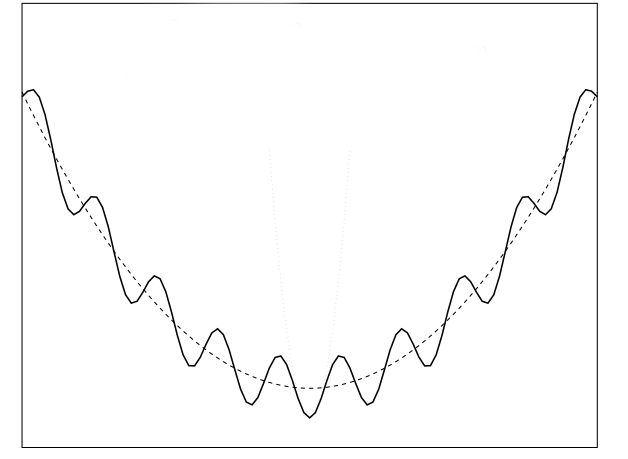
\includegraphics[trim = -1cm -3cm 0cm 0cm , clip, width=6cm,height=7cm]{Kap2/mult_min.png}%
\caption{Potencial en funci\'{o}n de la posici\'{o}n, a) mostrando la energ\'{i}a total $E$ y los cambios en la energ\'{i}a cin\'{e}tica y b) mostrando el modelo de m\'{u}ltiples m\'{i}nimos. } \label{fig:pot}
\end{figure}

Considerando la condici\'{o}n de equilibrio \eqref{eq:2} y despreciando desplazamientos de orden superior se tiene que:
\begin{equation}\label{eq:3}
V(\mathbf{q})=\frac{1}{2}\sum_{i,j=1}^{n}\frac{\partial^2 V }{\partial q_i\partial q_j}\bigg|_{\mathbf{q}=\mathbf{0}}q_i q_j
\end{equation}

Donde se identifican las constantes el\'{a}sticas como:
\begin{equation}\label{eq:4}
U_{ij}=\frac{\partial^2 V }{\partial q_i\partial q_j}\bigg|_{\mathbf{q}=\mathbf{0}}
\end{equation}

En t\'{e}rminos matriciales el potencial se puede escribir como:
\begin{equation}\label{eq:5}
V(\mathbf{q})=\frac{1}{2}\mathbf{q}^t\mathbf{U}\mathbf{q}
\end{equation}
En la ecuaci\'{o}n \eqref{eq:5} $\mathbf{q}$ es el vector columna formado por los desplazamientos de las posiciones de equilibrio para cada constituyente, i. e., $\mathbf{q}^t=(q_1,q_2,...q_n)$. Por otro lado la matriz de constantes el\'{a}sticas $\mathbf{H}$, es una matriz sim\'{e}trica debido a que la fuerza generalizada se considera conservativa, lo cual permite intercambiar el orden de las derivadas parciales.\\

Para las peque\~{n}as oscilaciones, no existen ligaduras dependientes expl\'{i}citamente de el tiempo (holon\'{o}micas) luego, la eneg\'{i}a cin\'{e}tica de los constituyentes s\'{o}lo depender\'{a} de los cuadrados de las velocidades generalizadas:
\begin{equation}\label{eq:6}
T=\frac{1}{2}\mathbf{q}^t\mathbf{M}\mathbf{q}
\end{equation}
Donde $\mathbf{M}$ es la masa generalizada, la cual se expresa en t\'{e}rminos de los factores de escala entre sistemas coordenados:
\begin{equation}\label{eq:7}
M_{jk}=\sum_{i=1}^{N} m_{i}\frac{\partial \mathbf{r_{i}} }{\partial q_j}\cdot\frac{\partial \mathbf{r_{i}} }{\partial q_k}
\end{equation}
La forma en que se escribir\'{a}n los elementos de la masa del sistema depende de la transformaci\'{o}n aplicada. Por ejemplo, en una dimensi\'{o}n las componentes de $\mathbf{q}$ se definen como:
\begin{equation}\label{eq:8}
q_i=x_i-x_{i0}
\end{equation}
En \eqref{eq:8} $x_i$ es la posici\'{o}n variable de la part\'{i}cula $i$ con respecto a un sistema fijo y $x_{i0}$ su posici\'{o}n de equilibrio. Para este caso particular \eqref{eq:7} se convierte en:
\begin{eqnarray}\label{eq:9}
M_{jk}&=&\sum_{i=1}^{N} m_{i} \delta_{ij}\delta_{ik}\nonumber \\
M_{jk}&=&m_{j} \delta_{jk}
\end{eqnarray}
La equaci\'{o}n \eqref{eq:9} dice que la matriz $\mathbf{M}$ es una matriz diagonal cuyas componentes son las masas del sistema.\\

Para el caso tridimensional, la matriz de masas del sistema es (Los detalles del c\'{a}lculo se encuentran en el anexo \ref{AnexoA}):
\begin{equation}
M_{jk}=\left( m_{3j-2}+m_{3j-1}+m_{3j} \right) \delta_{jk}
\end{equation}

\paragraph{Ecuaci\'{o}n de Movimiento}
El sistema satisface la ecuaci\'{o}n de un oscilador arm\'{o}nico, lo cual se muestra para las peque\~{n}as oscilaciones en \cite[Chapter~6]{Goldstein2001}:
\begin{equation}\label{eq:14}
\mathbf{M}\ddot{\mathbf{q}}+\mathbf{U}\mathbf{q}=\mathbf{0}
\end{equation}
Para convertir la ecuaci\'{o}n a la forma est\'{a}ndar se usan las coordenadas de masa ponderada (en ingl\'{e}s mass-weighted coordinates) las cuales cambian la escala en la que se mide la posici\'{o}n:
\begin{eqnarray}\label{eq:15}
\mathbf{r}&=&\mathbf{M}^{1/2}\mathbf{q}\\
\mathbf{K}&=&\mathbf{M}^{-1/2}\mathbf{U}\mathbf{M}^{-1/2}
\end{eqnarray}
Reemplazando dichas transformaciones en la ecuaci\'{o}n de movimiento se obtiene:
\begin{equation}\label{eq:16}
\ddot{\mathbf{r}}+\mathbf{K}\mathbf{r}=\mathbf{0}
\end{equation}
El efecto que tienen las coordenadas de masa ponderada sobre la energ\'{i}a cin\'{e}tica  es el de desaparecer la dependencia con la matriz de masas del sistema, que como se vi\'{o} puede resultar en una expresi\'{o}n tediosa. Las energias cin\'{e}tica y potencial en las nuevas coordenadas son:
\begin{eqnarray}\label{eq:19}
T&=&\frac{1}{2}\mathbf{q}^t\mathbf{M}\mathbf{q} \nonumber \\
T&=&\frac{1}{2}\mathbf{\dot{r}}^t\mathbf{M^{-1/2}}^t\mathbf{M}\mathbf{M^{1/2}}\mathbf{\dot{r}}\nonumber \\
T&=&\frac{1}{2}\mathbf{\dot{r}}^t \mathbf{\dot{r}}
\end{eqnarray}
\begin{eqnarray}\label{eq:20}
V(\mathbf{q})&=&\frac{1}{2}\mathbf{q}^t\mathbf{U}\mathbf{q} \nonumber \\
V(\mathbf{q})&=&\frac{1}{2}\mathbf{r}^t\mathbf{M^{-1/2}}^t\mathbf{U}\mathbf{M^{1/2}}\mathbf{r} \nonumber \\
V(\mathbf{q})&=&\frac{1}{2}\mathbf{r}^t\mathbf{K}\mathbf{r}
\end{eqnarray}
Una soluci\'{o}n (de prueba) a la ecuaci\'{o}n de movimiento es la oscilatoria, en la cual los constituyentes de la biomol\'{e}cula tienen la misma frecuencia $\omega$:
\begin{equation}\label{eq:17}
\mathbf{r}=\mathbf{a}e^{i\omega t}
\end{equation}
El vector $\mathbf{a}$ es denominado vector de amplitudes debido a que cada una de sus componentes corresponde a las amplitudes de cada mon\'{o}mero. Sus valores son fijos en el tiempo.\\

Al reemplazar la soluci\'{o}n de prueba en la ecuaci\'{o}n \eqref{eq:16} se convierte en un problema de autovalores y autovectores:

\begin{eqnarray}\label{eq:18}
\ddot{\mathbf{r}}&=&-\mathbf{K}\mathbf{r} \nonumber \\
\omega^2\mathbf{a}&=&\mathbf{K}\mathbf{a} \nonumber \\
\lambda_{k}\mathbf{a_{k}}&=&\mathbf{K}\mathbf{a_{k}}
\end{eqnarray}

En \eqref{eq:18} se ha definido $\lambda=\omega^2$ y posteriormente se ha agregado el sub\'{i}ndice $k$ para distinguir cada uno de los autovalores y autovectores que se encuentren en el problema \eqref{eq:18}.\\
Cuando cada uno de los mon\'{o}meros tiene la misma frecuencia, a cada frecuencia le corresponde un vector de amplitudes $\mathbf{a}$, cada uno de estos posibles vectores se les conoce como un \textit{modo normal de oscilaci\'{o}n}.\\

Ha de notarse que la soluci\'{o}n total no est\'{a} compuesta por un \'{u}nico modo, sino por la superposici\'{o}n de estos:
\begin{equation}\label{eq:tot}
\mathbf{r}=\sum_k\mathbf{a}_ke^{i\omega_k t}
\end{equation}

Cuando se tiene esta soluci\'{o}n y se desean conocer los modos normales, pueden aplicarse dos m\'{e}todos: El de la transformada de Fourier para conocer las frecuencias y la transformaci\'{o}n a las coordenadas normales; las coordenadas normales son un espacio en el cual se separan los movimientos compuestos.\\

Las coordenadas normales $\mathbf{\zeta}$ se definen como:
\begin{equation}
\mathbf{r}=\mathbf{T}\mathbf{\zeta}
\end{equation}
Donde $\mathbf{T}$ es una transformaci\'{o}n ortogonal  $\mathbf{T}\mathbf{T}^T=\mathbf{I}$ formada por los modos normales $\mathbf{a}_k$  pero modificados para que se cumpla la ortonormalidad. Cada componente de $\mathbf{\zeta}$ es:
\begin{equation}
\zeta_k=C_k e^{i\omega_k t}
\end{equation}
Es decir, las coordenadas normales $\zeta_k$ representan a un \'{u}nico modo normal de oscilaci\'{o}n, una \'{u}nica frecuencia. Mientras que las columnas de $\mathbf{T}$ proporcionan las direcciones en las que se da cada modo normal.\\


\subsubsection{Ensamble Estad\'{i}stico}
Cuando el sistema (biomol\'{e}cula) se encuentre a temperaturas fisiol\'{o}gicas, s\'{o}lo intercambiar\'{a} calor con los alrededores (ba\~{n}o t\'{e}rmico). Sin embargo, se ha demostrado  que a esta temperatura, la aproximaci\'{o}n arm\'{o}nica falla , \cite{Hayward2008}; por otro lado, a temperatura fisiol\'{o}gica el ensamble es cl\'{a}sico dependiendo del rango de frecuencias a analizar\cite{Sethna2006}, \cite{Cui2006}. En la figura \ref{fig:estad}, se observa el n\'{u}mero de nodos en funci\'{o}n de la frecuencia para diferentes prote\'{i}nas, para frecuencias menores que la frecuencia de vibraci\'{o}n del oscilador arm\'{o}nico a temperatura ambiente, se puede trabajar con la mec\'{a}nica cl\'{a}sica.\\
\begin{figure}
\centering%
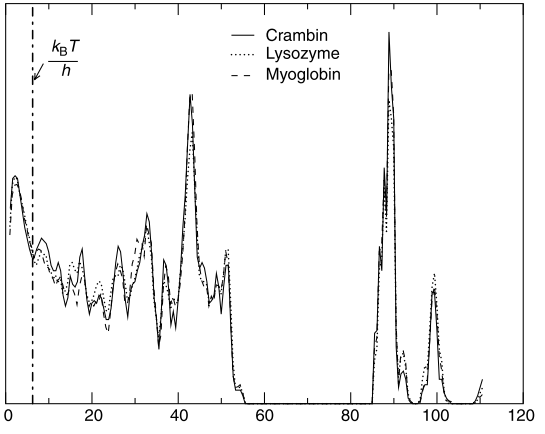
\includegraphics[scale=0.3]{Kap2/modos_vs_f.png}%
\put(-80,50){N\'{u}mero de modos}
\put(-45,-5){Frecuencia ($p\mathrm{s}^{-1}$)}
\caption{Desplazamientos de los nodos $i-j$ de su posici\'{o}n de equilibrio. Tomado de \cite{Cui2006}.} \label{fig:estad}
\end{figure}
Como \'{u}nicamente hay intercambio de energ\'{i}a y se trabaja a temperatura fisiol\'{o}gica, la estad\'{i}stica apropidada es la del ensamble can\'{o}nico. En el ensamble  can\'{o}nico se sigue la distribuci\'{o}n de probabilidad de Boltzmann:
\begin{equation}\label{eq:21}
p=\frac{\exp(-E_s/k_BT)}{Z}
\end{equation}
Donde $E_s$ es la energ\'{i}a del sistema y $Z$ la funci\'{o}n de partici\'{o}n. La funci\'{o}n de partici\'{o}n es el factor de normalizaci\'{o}n de la densidad de probabilidad y cuenta todos los posibles microestados a temperatura constante:
\begin{equation}\label{eq:22}
Z=\frac{1}{h^{n}}\int \mathrm{d}^n p\mathrm{d}^n q \exp \left [-H(\mathbf{p},\mathbf{q})/k_BT \right]
\end{equation}
En \eqref{eq:22}, $n=3N$ cuando el n\'{u}mero de coordenadas $q_i$ escogido es el mismo que el n\'{u}mero de coordenadas cartesianas.\\
Ha de notarse que la funci\'{o}n de partici\'{o}n en \eqref{eq:22} desacopla los momentos y las posiciones, ya que el hamiltoniano est\'{a} dado por la f\'{o}rmula $H=T+V$, donde la enger\'{i}a cin\'{e}tica depende s\'{o}lo de los momentos generalizados y  el potencial de las coordenadas generalizadas.\\

Se desarrolla \eqref{eq:22} teniendo en cuenta que $\mathbf{M}$ es diagonal:
\begin{eqnarray}\label{eq:23}
Z&=&\frac{1}{h^{n}}\int \mathrm{d}^n p\mathrm{d}^n q \exp \left [-\left( \mathbf{\dot{q}^t}\mathbf{M}\mathbf{\dot{q}}/2+\mathbf{q}^t\mathbf{U}\mathbf{q}/2\right)/k_BT \right]
\nonumber \\
Z&=&\frac{1}{h^{n}}\int \mathrm{d}^n p \exp \left [-\sum_i \frac{p_i^2}{2m_i}\right]
\int \mathrm{d}^n r \left( \prod_i \sqrt{m_i}\right)\exp \left[-\frac{1}{2}\mathbf{r}^t\mathbf{K}\mathbf{r}/k_BT \right]
\nonumber \\
Z&=&\frac{(2\pi)^{n/2}}{h^{n}}
\int \mathrm{d}^n r\exp \left[-\frac{1}{2}\mathbf{r}^t\mathbf{K}\mathbf{r}/k_BT \right] 
\end{eqnarray}
El resultado \eqref{eq:23} es el mostrado en \cite{Lezon2009} o en \cite{Sethna2006}:
\begin{equation}\label{eq:24}
Z=\frac{\left(k_BT\right)^{n/2}}{\hbar^{n}} \frac{1}{|\mathbf{K}|^{n/2}}
\end{equation}
Tomando $\hbar=1$ y teniendo en cuenta que el determinante de $\mathbf{K}$ es el producto de los autovalores no nulos, es decir, de las frecuencias al cuadrado:
\begin{eqnarray}\label{eq:25}
Z&=&\left(k_BT\right)^{n/2} \prod_{i=1}^{n}\frac{1}{\omega_i}
 \\
Z&=&\left(k_BT\right)^{n/2} |\mathbf{K^{-1}}|^{1/2}
\end{eqnarray}
Se observa que los modos de m\'{a}s bajas frecuencias contribuyen m\'{a}s a la funci\'{o}n de partici\'{o}n.
\section{Descripciones de los Movimientos Globales}
\subsection{ENMs}
\subsubsection{Modelos de Redes Anisotr\'{o}picas (ANM)}
Como se ha dicho, la aproximaci\'{o}n a segundo orden del potencial, minimizaci\'{o}n, \eqref{eq:5} es cambiada por un potencial de Hooke en el cual se tienen en cuenta las distancias en lugar de los desplazamientos alrededor del equilibrio y tambi\'{e}n se pueden tener en cuenta diferentes constantes el\'{a}sticas entre diferentes nodos:
\begin{equation}\label{eq:26}
V=
   \frac{1}{2}\sum_{
   i,j>i  
   }
   \gamma_{ij}\left(R_{ij}-R_{ij}^0\right)^2
\end{equation}
\begin{equation*}
\mbox{			Con		} R_{ij},R_{ij}^0<R_c  
\end{equation*}

Donde $R_{ij}^0$ es la distancia de equilibrio entre los nodos $i-j$ de la red, $R_{ij}$ su distancia variable y $\gamma_{ij}$ las constantes el\'{a}sticas entre los nodos $i-j$. Como se ilustra en la figura \ref{fig:res}, el t\'{e}rmino $R_{ij}-R_{ij}^0$ es la elongaci\'{o}n del resorte, lo cual es diferente a la resta de los desplazamientos, ecuaci\'{o}n \eqref{eq:3}; entonces no se est\'{a} aproximando el potencial ni se requiere una minimizaci\'{o}n de la energ\'{i}a, como se ha recalcado, s\'{o}lo se cambia la forma del potencial.\\

Se requiere que $j>i$ para que no aparezca repetido el t\'{e}rmino $\left(R_{ij}-R_{ij}^0\right)^2$ con $\left(R_{ji}-R_{ji}^0\right)^2$   ya que representan la misma interacci\'{o}n, de ser as\'{i}, se vuelven obsoletas las constantes el\'{a}sticas $\gamma_{ij}$ con $j<i$. Sin embargo, el potencial tambi\'{e}n puede escogerse dejando los t\'{e}rminos repetidos y redefiniendo la matriz de constantes el\'{a}sticas como una matriz sim\'{e}trica, esto es: $\gamma_{ij}=\gamma_{ji}$. Escogiendo el potencial de esta manera, como es usal en la literatura \cite{Rader2006}, queda de la forma:
\begin{equation}\label{eq:26}
V_{ANM}=
   \frac{1}{2}\sum_{
   i\neq j=1  
   }
   \gamma_{ij}\left(R_{ij}-R_{ij}^0\right)^2
\end{equation}
\begin{eqnarray*}
\mbox{			Con		} R_{ij},R_{ij}^0<R_c \\
\mbox{			y		} \gamma_{ij}=\gamma_{ji}
\end{eqnarray*}
\begin{figure}
\centering%
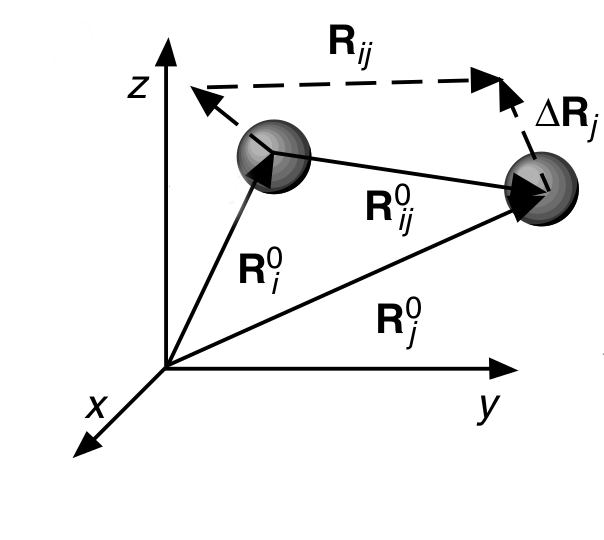
\includegraphics[scale=0.3]{Kap2/resorte.png}%
\caption{Desplazamientos de los nodos $i-j$ de su posici\'{o}n de equilibrio. Tomado de \cite{Rader2006}.} \label{fig:res}
\end{figure}
Existe un servidor web \cite{Eyal2015} basado en ANM que permite ver los movimientos globales de una prote\'{i}na o de un \'{a}cido nucleico y permite obtener informaci\'{o}n como los autovalores, los factores-B, las correlaciones entre otras.\footnote{ Recurso disponible en \url{http://anm.csb.pitt.edu/cgi-bin/anm2/anm2.cgi}}
\paragraph{Matriz Hessiana}
El c\'{a}lculo de la matriz de segundas derivadas $\mathbf{U}$ para el an\'{a}lisis de modos normales, si parte de una minimizaci\'{o}n de la energ\'{i}a.  Las derivadas se calculan v\'{i}a el potencial anisotr\'{o}pico \eqref{eq:26}, para el presente caso la matriz $\mathbf{U}$ es llamada $\mathbf{\mathcal{H}}$. La matriz $\mathbf{\mathcal{H}}$ es de tama\~{n}o $3N\times3N$ con $N$ el n\'{u}mero de residuos y est\'{a} constituida por $N\times N$ submatrices de tama\~{n}o $3\times3$ llamadas $\mathbf{H}_{ij}$:
\begin{equation}\label{eq:34}
\mathbf{\mathcal{H}}=\{H_{ij}\} \mbox{		con	}i,j=1,...,N
\end{equation}
Los elementos de $\mathbf{H}_{ij}$ son:
\begin{equation}\label{eq:35}
\mathbf{H}_{ij}=\left(
\begin{array}{ccc}
 \partial_{xi}\partial_{xj} V & \partial_{xi}\partial_{yj} V & \partial_{xi}\partial_{zj} V \\
 \partial_{yi}\partial_{xj} V & \partial_{yi}\partial_{yj} V & \partial_{yi}\partial_{zj} V \\
 \partial_{zi}\partial_{xj} V & \partial_{zi}\partial_{yj} V & \partial_{zi}\partial_{zj} V
\end{array}
\right)
\end{equation}

Calculando algunas de estas derivadas y definiendo $x_{ik}=x_k-x_i$, $y_{ik}=y_k-y_i$ y $z_{ik}=z_k-z_i$ se obtiene (Caso $i\neq j$):
\begin{equation}\label{eq:36}
\frac{\partial V }{\partial y_k}=\sum_j\frac{\gamma_{jk}\left(R_{kj}-R_{kj}^0\right)y_{kj}}{R_{kj}}
\end{equation}
\begin{equation}\label{eq:37}
\frac{\partial^2 V }{\partial x_i\partial y_j}\bigg|_{R_{ij}=R_{ij}^0}=-\frac{\gamma_{ij}x_{ij}y_{ij}}{R_{ij}^2}
\end{equation}
\begin{equation}\label{eq:38}
\frac{\partial^2 V }{\partial x_i\partial x_j}\bigg|_{R_{ij}=R_{ij}^0}=-\frac{\gamma_{ij}x_{ij}^2}{R_{ij}^2}
\end{equation}
De forma an\'{a}loga se encuentran los otros elementos de $\mathbf{H}_{ij}$ con lo cual los superelementos no diagonales de $\mathbf{\mathcal{H}}$ quedan escritos como \cite{Lezon2009}:
\begin{equation}\label{eq:35}
\mathbf{H}_{ij}=-\frac{\gamma_{ij}}{R_{ij}^2}\left(
\begin{array}{ccc}
 x_{ij}^2 & x_{ij}y_{ij} & x_{ij}z_{ij}\\
 y_{ij}x_{ij} & y_{ij}^2 & y_{ij}z_{ij} \\
 z_{ij}x_{ij} &z_{ij}y_{ij} & z_{ij}^2
\end{array}
\right)
\end{equation}


Para los superelementos $\mathbf{H}_{ii}$ que se encuentran en la diagonal, algunos de sus elementos son:
\begin{eqnarray}\label{eq:39}
\frac{\partial^2 V }{\partial x_i^2}\bigg|_{R_{ij}=R_{ij}^0}=-\sum_{j\neq i}\gamma_{ij}\left(\frac{x_{ij}^2}{R_{ij}^2}\right) \nonumber \\
\frac{\partial^2 V }{\partial x_i^2}\bigg|_{R_{ij}=R_{ij}^0}=-\sum_{j\neq i} H_{ij,xx}
\end{eqnarray}
En \eqref{eq:39}, $H_{ij,xx}$ es el primer elemento de la submatriz $\mathbf{H}_{ij}$. El resultado \eqref{eq:39} puede generalizarse para todos los superelementos de la diagonal, ver \cite{Lezon2009}:
\begin{eqnarray}\label{eq:40}
\mathbf{H}_{ii}=\sum_{j\neq i}\mathbf{H}_{ij}
\end{eqnarray}
Una vez obtenida la matriz Hessiana, es necesario calcular sus autovalores y autovactores, de la misma forma que en NMA, ya que esto describe los movimientos de la biomol\'{e}cula. La diagonalizaci\'{o}n de $\mathcal{H}$ lleva a lo sumo $3N-6$ modos normales no nulos, como se demuestra en \cite{Tirion1996}. Los 6 modos normales restantes, corresponden a las rotaciones y traslaciones de un cuerpo r\'{i}gido; se puede escoger un sistema fijo en la molecula y que rote con ella.\\

El t\'{e}rmino de la distancia de corte $R_c$ puede ser incluido en las constantes el\'{a}sticas, es decir, $\gamma_{ij}=0$ si  $R_{ij}>R_c$ sino $\gamma_{ij}\neq 0$. Adicional a esto, las constantes el\'{a}sticas pueden ser iguales (isotr\'{o}picas): $\gamma_{ij}=\gamma$ si  $R_{ij}<R_c$ de lo contrario  $\gamma_{ij}=0$.
\subsubsection{Modelo de Redes Gaussianas (GNM)}
El modelo se denomina gaussiano debido a que las desviaciones del equilibrio o fluctuaciones con respecto al equlibrio son gaussianas e isotr\'{o}picas \cite{Rader2006}. Se requieren dos par\'{a}metros para describir el modelo: Una misma constante el\'{a}stica $\gamma$ para todas las unidades de la biomol\'{e}cula y una distancia de corte a partir de la cual no se ejerce el potencial.\\
Contrario al ANM, en el modelo de redes gaussianas se consideran las desviaciones del equilibrio como desplazamientos:
\begin{equation}\label{eq:27}
V_{GNM}=\frac{\gamma}{2}\sum_{i,j=1}^{N}\Gamma_{ij}\left(\textbf{R}_{ij}-\textbf{R}_{ij}^0\right)^2
\end{equation}
Al ser $\gamma_{ij}$ una matriz de constantes el\'{a}sticas, se incluyen en la sumatoria los elementos $\Gamma_{ij}$ donde $\gamma_{ij}=\gamma\Gamma_{ij}$. $\Gamma_{ij}$ representa la simetr\'{i}a de la matriz $ \mathbf{\gamma}$ y como se puede ver en \cite{Rader2006}, la topolog\'{i}a de la red.\\

Ya que $\textbf{R}_{ij}=\textbf{R}_{j}-\textbf{R}_{i}$ y definiendo $\Delta\textbf{R}_{i}=\textbf{R}_{i}-\textbf{R}_{i}^0$ se tiene que  $\textbf{R}_{ij}-\textbf{R}_{ij}^0=\Delta\textbf{R}_{j}-\Delta\textbf{R}_{i}$, el potencial gaussiano se puede escribir en t\'{e}rminos de los desplazamientos individuales:
\begin{eqnarray}\label{eq:34}
V_{GNM}&=&\frac{\gamma}{2}\sum_{i\neq j=1}^{N}\Gamma_{ij}\left( \Delta\textbf{R}_{j}-\Delta\textbf{R}_{i}\right)^2 \nonumber \\
V_{GNM}&=&\frac{\gamma}{2}\sum_{i\neq j=1}^{N}\Gamma_{ij}\left[\left(\Delta x_j-\Delta x_i \right)^2+\left(\Delta y_j-\Delta y_i \right)^2+\left(\Delta z_j-\Delta z_i \right)^2 \right] \nonumber \\
V_{GNM}&=&\frac{\gamma}{2}\sum_{i\neq j=1}^{N}\Gamma_{ij}\left[\left(\Delta x_{ij}\right)^2+\left(\Delta y_{ij}\right)^2+\left(\Delta z_{ij}\right)^2 \right]
\end{eqnarray}
Escribiendo \eqref{eq:34} en forma matricial se tiene:
\begin{equation}\label{eq:35}
V_{GNM}=\frac{\gamma}{2}\left(\Delta\mathbf{X}^T\mathbf{\Gamma}\Delta\mathbf{X}+\Delta\mathbf{Y}^T\mathbf{\Gamma}\Delta\mathbf{Y}+\Delta\mathbf{Z}^T\mathbf{\Gamma}\Delta\mathbf{Z} \right)
\end{equation}
Para garantizar que $\Gamma_{ij}$ sea adimensional, se escogen (no de forma \'{u}nica) los elementos fuera de la diagonal de acuerdo al procedimiento descrito a continuaci\'{o}n.\\

N\'{o}tese que los t\'{e}rminos cuadr\'{a}ticos por cada componente pueden expandirse:
\begin{eqnarray}\label{eq:36}
\sum_{i\neq j=1}^{N}\Gamma_{ij}\left(\Delta x_{ij}\right)^2&=&\sum_{i\neq j=1}^{N}\Gamma_{ij}\left(\Delta x_{i}^2+\Delta x_{j}^2-2\Delta x_{i}\Delta x_{j}\right) \nonumber \\
&=&2\sum_{i\neq j=1}^{N}\Gamma_{ij}\Delta x_{i}^2-2\sum_{i\neq j=1}^{N}\Delta x_{i}\Gamma_{ij}\Delta x_{j}
\end{eqnarray}

Existe un servidor web basado en GNM que permite ver los movimientos globales de una prote\'{i}na o de un \'{a}cido nucleico y permite obtener informaci\'{o}n como los autovalores, los factores-B, las correlaciones entre otras.\footnote{ Recurso disponible en \url{http://web.archive.org/web/20070615210550/http://ignm.ccbb.pitt.edu/GNM_Online_Calculation.htm}}

\subsection{An\'{a}lisis por Componentes Principales (PCA)}
Sea $\mathbf{x(t)}$ la trayectoria en forma de vector columna de $3N$ componentes que tiene las posiciones a cada instante de tiempo de todos los \'{a}tomos. La matriz de covarianza, en este caso, es aqu\'{e}lla que mide la dependencia entre cada una de las variables ($3N$ componentes) y cuyos elementos de la diagonal son las varianzas de dichas variables.\\

Matriz de covarianza:
\begin{equation}\label{eq:28}
C=\langle(\mathbf{x(t)}-\langle\mathbf{x}\rangle)(\mathbf{x(t)}-\langle\mathbf{x}\rangle)^T\rangle
\end{equation}

En \eqref{eq:29}, la media es calculada para la trayectoria en todos los tiempos.\\
La matriz de covarianza puede ser expresada en t\'{e}rminos de sus autovalores  $\lambda_i$ y sus autovectores $\mathbf{t_i}$, con $i<3N+1$.
\begin{equation*}
\mathbf{C}\mathbf{t_i}=\lambda_i\mathbf{t_i}
\end{equation*}
Tomando $\Lambda={\lambda_i}$, la matriz diagonal formada por los autovalores y $\mathbf{T}=\left(\mathbf{t_1},\mathbf{t_2},...,\mathbf{t_{3N}}\right)$ como la matriz cuyas columnas son los autovectores, escritas de tal manera que los autovalores esten ordenados de mayor a menor y los autovectores ordenados de acuerdo a los autovalores entonces:
\begin{equation}\label{eq:29}
\mathbf{\Lambda}=\mathbf{T}^T\mathbf{C}\mathbf{T}
\end{equation}
Donde se ha tenido en cuenta que $\mathbf{T}^{-1}=\mathbf{T}^T$. Expresado de otra forma:
\begin{equation}\label{eq:30}
\mathbf{C}=\mathbf{T}\mathbf{\Lambda} \mathbf{T}^T
\end{equation}
La esencia de un PCA es descartar los modos menos relevantes que corresponden a los autovalores m\'{a}s peque\~{n}os y generar un nuevo conjunto de datos de menor tama\~{n}o a partir de estos (componentes principales). En \cite{Amadei1993} se demuestra que las desviaciones m\'{a}s grandes corresponden a los autovalores m\'{a}s grandes, por tanto, se trabaja s\'{o}lamente con los autovalores m\'{a}s grandes. \\

Dejando s\'{o}lamente en $\mathbf{T}$ los $M$ autovectores o columnas m\'{a}s relevantes, se define la matriz de las componentes principales $\mathbf{P}=\left(\mathbf{p_1},\mathbf{p_2},...,\mathbf{p_{M}}\right)$, donde $M<3N$ como:
\begin{eqnarray}\label{eq:31}
\mathbf{P}&=&\mathbf{T}^T(\mathbf{x(t)}-\langle\mathbf{x}\rangle)^T \nonumber \\
\mathbf{P}&=&(\mathbf{x(t)}-\langle\mathbf{x}\rangle)\mathbf{T}
\end{eqnarray}
O en t\'{e}rminos de cada componente principal:
\begin{equation}\label{eq:32}
\mathbf{p_i}=\mathbf{t_i}^T(\mathbf{x(t)}-\langle\mathbf{x}\rangle)^T
\end{equation}
Si se desea volver a los datos originales hay que realizar la transformaci\'{o}n inversa:
\begin{equation}\label{eq:33}
\mathbf{x(t)}^T=\mathbf{T}\mathbf{P}+\langle\mathbf{x}\rangle^T
\end{equation}
\subsection{Modelos de Bloque R\'{i}gido (BNM o RTB)}
Los modos normales de los bloques r\'{i}gidos tienen una dimensi\'{o}n de tama\~{n}o $n_b$ con respecto a los de un NMA, $3N$. Los modos normales de bloque r\'{i}gido se definen a partir de una transformaci\'{o}n denominada $\mathbf{P}$ del espacio de las ${q_i}$ al de los bloques r\'{i}gidos $r_i'$.\\

La ecuaci\'{o}n de movimiento es:

\section{Comparaci\'{o}n Entre distintos modelos}
\subsection{Diferencias entre GNM y ANM}
\section{Clasificaci\'{o}n Modelos Te\'{o}ricos}
\begin{figure}
\centering%
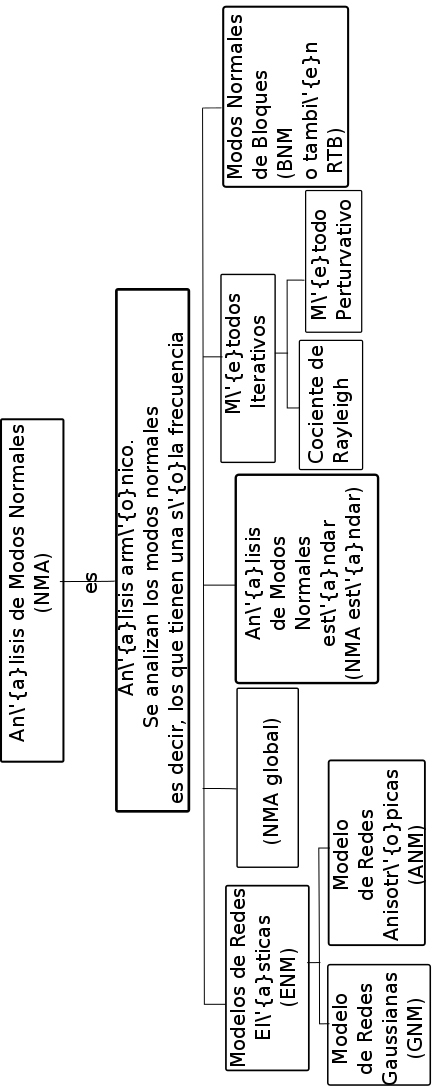
\includegraphics[scale=0.4]{Kap2/mapa.png}%
\caption{Mapa conceptual en el que se dividen los movimientos locales de los movimientos globales y mostrando cada tipo de movimiento global utilizado} \label{fig:movs}
\end{figure}